\documentclass[conference]{IEEEtran}
\IEEEoverridecommandlockouts
% The preceding line is only needed to identify funding in the first footnote. If that is unneeded, please comment it out.
\usepackage{cite}
\usepackage{amsmath,amssymb,amsfonts}
\usepackage{algorithmic}
\usepackage{graphicx}
\usepackage{textcomp}
\usepackage{xcolor}
\usepackage{tabularx}
\usepackage{multirow}
\usepackage{graphics} % for pdf, bitmapped graphics files
\usepackage{subfig}
\usepackage{subcaption}
\usepackage{hyperref}
\usepackage{academicons}
\usepackage{xcolor}
\usepackage{listings}
\usepackage{tabularx} % Asegúrate de incluir este paquete

\usepackage{tikz}
\usetikzlibrary{shapes.geometric, arrows}

\usetikzlibrary{shapes.geometric, arrows}

\tikzstyle{startstop} = [rectangle, rounded corners, minimum width=3cm, minimum height=1cm,text centered, draw=black, fill=red!30]
\tikzstyle{process} = [rectangle, minimum width=3cm, minimum height=1cm, text centered, draw=black, fill=blue!30]
\tikzstyle{arrow} = [thick,->,>=stealth]


\def\BibTeX{{\rm B\kern-.05em{\sc i\kern-.025em b}\kern-.08em
		T\kern-.1667em\lower.7ex\hbox{E}\kern-.125emX}}

% Color Enlace
\definecolor{colorEnlace}{RGB}{0, 0, 0}
\hypersetup{
	colorlinks=true,
	linkcolor=colorEnlace,
	citecolor=colorEnlace,
	urlcolor=colorEnlace,
	pdfauthor={Davis Bremdow Salazar Roa},
	pdftitle={Telecomunicaciones I - Análisis en la señal de ruido}
}
\definecolor{mybg}{rgb}{0.97,0.97,0.97}
\definecolor{mygray}{gray}{0.4}
\definecolor{mygreen}{rgb}{0,0.6,0}
\definecolor{myblue}{rgb}{0,0,0.8}
\definecolor{mypurple}{rgb}{0.58,0,0.82}
\definecolor{myred}{rgb}{0.7,0,0}

\lstdefinelanguage{MatlabEnhanced}{
	language=Matlab,
	morekeywords={[2]linspace,plot,title,xlabel,ylabel,legend,grid},
	morekeywords={[3]sin,cos,exp,log,sqrt},
	keywordstyle=\color{myblue}\bfseries,
	keywordstyle=[2]\color{mypurple},
	keywordstyle=[3]\color{myred},
	commentstyle=\color{mygreen}\itshape,
	stringstyle=\color{mygray},
	morecomment=[l]%
}

\lstset{
	language=MatlabEnhanced,
	backgroundcolor=\color{mybg},
	frame=single,
	basicstyle=\ttfamily\small,
	showstringspaces=false,
	numbers=none,              %
	xleftmargin=0pt,           %
	framexleftmargin=0pt,      
	framexrightmargin=0pt,
	framextopmargin=2pt,
	framexbottommargin=2pt,
	breaklines=true,
	tabsize=1,
}

% Control 
\usepackage{amsmath}
\begin{document}
	
	\title{Análisis de Ruido en una señal FM}
	\author{
		\makebox[\textwidth][c]{\large\textbf{Universidad Nacional de San Antonio Abad del Cusco}}\\
		\makebox[\textwidth][c]{\normalsize\textit{Escuela profesional de Ingeniería Electrónica}}\\
		\makebox[\textwidth][c]{\normalsize\textit{Ing. Milton Velasquez curo}}\\
		\makebox[\textwidth][c]{\normalsize\textit{Telecomunicaciones I}}\\
		\and
		\IEEEauthorblockN{Ruth Juana Espino Puma - 185746}
		\IEEEauthorblockA{Estudiante de Ingeniería Electrónica \\
			Cusco, Perú \\
			184657@unsaac.edu.pe}
		\and
		\IEEEauthorblockN{Aaron Coyla Quispe - 200832}
		\IEEEauthorblockA{Estudiante de Ingeniería Electrónica \\
			Cusco, Perú \\
			200832@unsaac.edu.pe}
		\and
		\IEEEauthorblockN{Davis Bremdow Salazar Roa - 200353}
		\IEEEauthorblockA{Estudiante de Ingeniería Electrónica \\
			Cusco, Perú \\
			200353@unsaac.edu.pe}
		
	}
	
	\maketitle
	\begin{abstract}
		This work studies the effect of noise on FM communication systems using GNU Radio and USRP devices. An FM transmitter and receiver were implemented with adjustable parameters such as carrier frequency and modulation index ($\beta$). Measurements were performed with a FieldFox spectrum analyzer, varying the distance between the noise source and the receiver. Data was processed in MATLAB using peak discrimination to estimate the noise floor. Results show that noise increases significantly at shorter distances, with the highest interference around 100 cm. The experiment confirms how external noise degrades FM signal quality and demonstrates the usefulness of GNU Radio for real-time testing of robust wireless systems.	
	\end{abstract}
	
	\begin{IEEEkeywords}
		Modulación FM, SNR
	\end{IEEEkeywords}
	
	%% Contenido del documento
	\section{Introducción.}
	La modulación FM, es una técnica de modulación en la que la frecuencia de la señal portadora varía en función de la amplitud de la señal de información. Este tipo de modulación es ampliamente utilizada en radiodifusión de alta fidelidad, comunicaciones de radio y sistemas inalámbricos.
	El análisis de ruido en sistemas de comunicación es esencial porque el ruido puede bajar la calidad de la señal recibida, afectando la precisión y la eficiencia del sistema. Comprender cómo se comporta el ruido permite crear sistemas más robustos, elegir técnicas de modulación adecuadas y aplicar métodos de filtrado y corrección de errores.
	\section{Antecedentes.}
	El análisis del ruido en sistemas de comunicación ha sido objeto de múltiples estudios debido a su impacto directo en el rendimiento de los receptores, especialmente en arquitecturas basadas en software. Uno de los trabajos más relevantes en esta línea es el realizado por Khanzadi, quienes desarrollaron un modelo matemático realista del ruido de fase (PN) en osciladores, considerando tanto fuentes de ruido blanco como de ruido coloreado. A partir de este modelo, los autores establecieron una relación directa entre las mediciones espectrales de un oscilador (en forma de espectro de banda lateral única) y el rendimiento óptimo de un sistema de comunicación, medido mediante el Error Vector Magnitude (EVM). El estudio demuestra que, en sistemas de alta velocidad, el ruido blanco alejado de la portadora tiene un efecto más significativo que el ruido acumulado cercano a esta, y que el ruido tipo $1/f^3$ es más predecible y menos perjudicial que el de tipo $1/f^2$. Este enfoque permite no solo evaluar el impacto del ruido en el sistema, sino también ofrecer criterios para el diseño de osciladores más eficientes.
	Por otro lado, la implementación práctica de sistemas de radio definidos por software (SDR) ha permitido validar muchos de estos modelos teóricos. En este contexto, se destaca el trabajo de Sharma, quien llevó a cabo la implementación en tiempo real de un sistema CDMA basado en códigos ZCZ (Zero Correlation Zone) utilizando GNU Radio y placas USRP. La investigación partió de una simulación previa en MATLAB y abordó los desafíos de trasladar dicho entorno a una plataforma SDR real, donde el control preciso del sincronismo, la longitud variable de los paquetes y la gestión de múltiples usuarios resultaron fundamentales. El sistema logró una comunicación asincrónica multiusuario sin interferencia significativa, siempre que las diferencias temporales entre los usuarios se mantuvieran dentro de la zona de correlación cero. Este estudio evidencia la capacidad de GNU Radio como herramienta eficaz para implementar y evaluar esquemas de transmisión robustos frente a interferencias y ruido.
	
	\section{ Objetivos }
	
	\begin{itemize}
		\item Implementación a nivel digital de un receptor y transmisor FM mediante el software GNU Radio
		\item Análisis en el nivel del piso de ruido en relación a un generador de acústico de ruido frente a la distancia.
		\item Determinar la distancia crítica para un nivel de ruido significativo en el piso de ruido inicial.
	\end{itemize}
	
	\section{Marco Teorico}
	
	\subsection{Modulacion en frecuencia.}
	La modulación en frecuencia (FM) es una técnica utilizada para transmitir información a través de una variación en la frecuencia de una onda portadora. Esta técnica es frecuentemente empleada en la transmisión de señales de radio, donde se modula la frecuencia de la onda en función de la señal de audio que se desea transmitir. La FM ofrece mejor calidad de sonido y mayor resistencia a las interferencias y ruidos que la modulación en amplitud (AM).
	
	\subsection*{Características de la Modulación FM}
	\begin{itemize}
		\item \textbf{Señal Portadora:} Consiste en una onda sinusoidal de alta frecuencia que transporta la señal moduladora.
		\item \textbf{Señal Moduladora:} Es la señal de información que se desea transmitir.
		\item \textbf{Ancho de Banda:} Representa el rango de frecuencias que ocupa la señal modulada.
		\item \textbf{Relación de Modulación:} Indica la relación entre la frecuencia máxima y mínima de la onda modulada.
		\item \textbf{Relación Señal/Ruido:} Es la relación entre la potencia de la señal modulada y la potencia del ruido.
	\end{itemize}
	
	\subsection{Fundamentos de Ruido}
	El ruido es una perturbación, señal  no deseada que interfiere en la comunicación, resulta de la mezcla de una señal útil con algún tipo de sistema de comunicación o proceso. También puede ser causada por una variedad de fuentes como interferencias electromagnéticas, fluctuaciones de voltajes, componentes electrónicos en mal estado.
	El ruido puede ser periodico o aleatorio,su espectro de frecuencia puede ser continuo o discreto según se menciona \cite{stremler2006}. El nivel de potencia del ruido se mide en decibelios (dB) y se expresa como la relación entre la potencia del ruido y la potencia de la señal útil.
	
	\subsubsection*{Tipos de Ruido en sistemas de comunicacion.}
	\begin{itemize}
		\item Ruido térmico o ruido de Johnson-Nyquist: Es un tipo de ruido generado por la agitación térmica de los electrones en un conductor. Independiente la frecuencia y su nivel de potencia aumenta con la temperatura.
		\item Ruido de intermodulación: Producido cuando dos o más señales de diferentes frecuencias se mezclan en un dispositivo no lineal, genera nuevas frecuencias no deseadas.
		\item Ruido impulsivo o ruido de ráfaga: Se genera por señales de corta duración y alta amplitud, como los rayos y los pulsos electromagnéticos.
		\item Ruido de fase: Se produce cuando la fase de la señal se desvía aleatoriamente.
		\item Ruido de cuantización: Se produce en los sistemas de conversión analógico-digital debido a la imprecisión en la medición de la señal analógica. Puede ser reducido aumentando la resolución del conversor.     
	\end{itemize}
	\subsection{Razón señal a ruido en la recepción FM}
	En los sistemas de modulación en frecuencia (FM), la razón señal a ruido (S/R) es una medida de la calidad de la señal recuperada. Esta se define como el cociente entre la potencia media de la señal útil y la potencia media del ruido a la salida del receptor.
	\subsection*{Modelo de receptor FM}
	Un receptor idealizado de FM incluye los siguientes bloques:
	\begin{itemize}
		\item \textbf{Amplificador limitador}: elimina las variaciones de amplitud de la señal, suprimiendo el ruido de amplitud.
		\item \textbf{Discriminador}: convierte las variaciones de frecuencia en voltaje proporcional a la señal moduladora.
	\end{itemize}
	\subsection*{Señal de salida sin ruido}
	Si la señal moduladora es \( f(t) \), y la constante del discriminador es \( k_f \), entonces la salida ideal del discriminador es:
	\[
	s(t) = k_f f(t)
	\]
	La potencia media de la señal como se indica en \cite{lazaro_teoria_telecom} en la salida es:
	\[
	S_o = k_f^2 E[f^2(t)]
	\quad \text{(Ec. 6.101)}
	\]
	\subsection*{Ruido en la salida del discriminador}
	Asumiendo ruido blanco de banda limitada, la potencia media del ruido a la salida es:
	\[
	N_o = \frac{3\pi^2 n_0 B^3}{A^2}
	\quad \text{(Ec. 6.110)}
	\]
	Donde:
	\begin{itemize}
		\item \( n_0 \): densidad espectral de potencia del ruido en la entrada
		\item \( B \): ancho de banda del sistema
		\item \( A \): amplitud de la portadora
	\end{itemize}
	\subsection*{Razón señal a ruido a la salida}
	Combinando las ecuaciones anteriores, la razón señal a ruido (S/R) en la salida es:
	\[
	\frac{S_o}{N_o} = \frac{k_f^2 E[f^2(t)] A^2}{3\pi^2 n_0 B^3}
	\quad \text{(Ec. 6.112)}
	\]
	Para una señal senoidal \( f(t) = a \cos(\omega_m t) \), se tiene:
	\[
	\frac{S_o}{N_o} = \frac{3}{2} \left(\frac{\Delta f}{B}\right)^2 \frac{S_i}{N_i}
	\quad \text{(Ec. 6.117)}
	\]
	Donde:
	\begin{itemize}
		\item \( \Delta f \): desviación pico de frecuencia
		\item \( \frac{S_i}{N_i} \): razón señal a ruido en la entrada
	\end{itemize}
	
	
	\section{ Metodología }
	
	Para poder cuantizar la influencia del generador de ruido en la demodulación FM, es de vital importancia poder modificar los parámetros de una señal FM, siendo que dentro de ello se debe considerar, el ancho de banda de la señal de información, la desviación máxima estándar y en función a ello el índice de modulación, además para poder trabajar dentro del ancho de banda de influencia del dispositivo de ruido también fue necesario controlar la frecuencia de transmisión.
	
	En tal sentido para este propósito se definieron 2 proyectos en el software GNU Radio que constituyen a un transmisor y demodulador FM los cuales pudieron facilitar la variación de parámetros.
	
	\subsection{ Transmisor FM }
	
	En la parte del transmisor FM se definió una modulación WBFM (Wide Band FM) esto con la finalidad de poder modificar el valor de $\beta$ o índice de modulación en el intervalo entre 0 y 10, en la figura \ref{fig:transmisor-fm} se muestra un esquema gráfico para este propósito en el cual para la transmisión se hace uso del bloque WBFM el cual internamente realiza el proceso de mezclado para la generación de una señal FM,, además también se hicieron uso  2
	
	
	\begin{figure}[h]
		\centering
		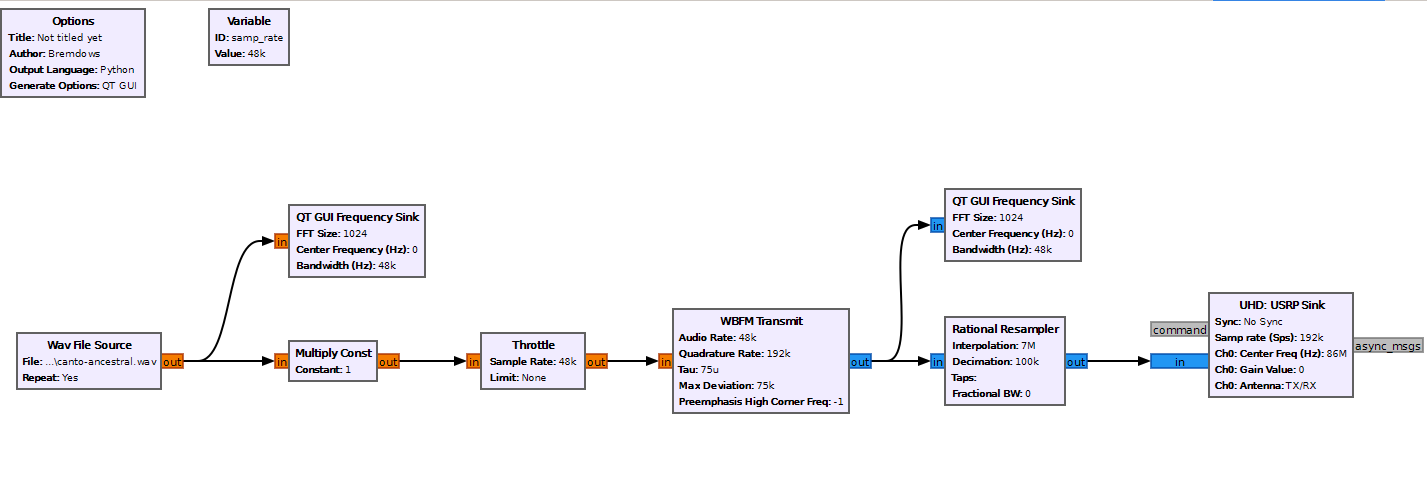
\includegraphics[width=0.5\textwidth]{media/transmisor-fm}
		\caption{SDR: Transmisor FM - GNU Radio}
		\label{fig:transmisor-fm}
	\end{figure}
	
	
	\subsection{ Receptor FM }
	
	El bloque receptor FM, se considero como elemento de validación de frecuencia y potencia de la señal transmitida, este a su vez estuvo compuesto por un bloque de entrada o de recepción perteneciente al USRP 2910 / 2920, un bloque para modifica la tasa de muestreo (Rational Resampler) para luego conectar estas 2 etapas previas con el bloque de demodulación FM (WBFM Receive), finalmente debido a la alta tasa de muestreo en la recepción al momento de reproducir la señal sintonizada, fue necesario volver a modificar la tasa de muestreo para adecuarla al estándar de 48k [Hz].
	
	\begin{figure}[h]
		\centering
		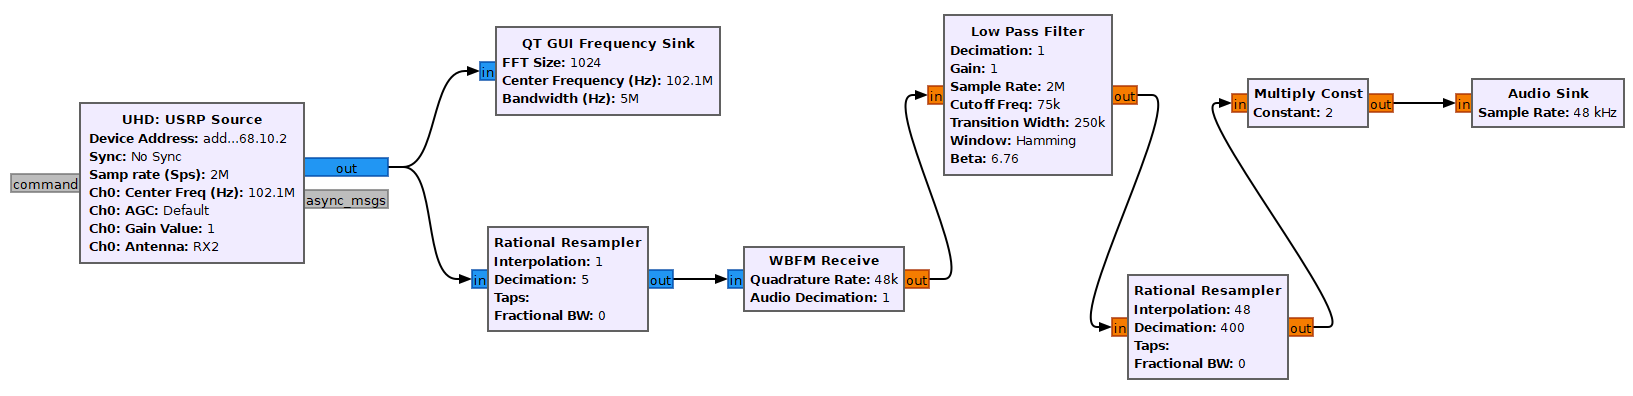
\includegraphics[width=0.5\textwidth]{media/receptor-fm}
		\caption{Receptor FM - GNU Radio}
		\label{fig:receptor-fm}
	\end{figure}
	
	En la figura \ref{fig:receptor-fm} se muestra el esquema general de los bloques utilizados en GNU Radio, en el cual se considera el bloque de recepción perteneciente al USRP, un bloque de ajuste en la frecuencia de muestreo, un bloque demodulador WBFM, el filtro de salida y finalmente un ajuste en el tasa de muestreo para ajustarla al archivo de audio.
	
	En función a estos bloques constitutivos se procedió con el experimento
	
	\section{Desarrollo del experimento}
	
	El procedimiento para realizar el experimento del efecto del ruido en modulación FM fue el siguiente
	
	\begin{enumerate}
		\item Medición de la potencia de piso de ruido
		\item Medición de la potencia añadiendo una fuente de ruido pero sin transmisión
		\item Medición de la potencia realizando una transmisión con un $\beta=5$ y añadiendo ruido.
		\item Medición de la potencia realizando una transmisión con un $\beta=6$ y añadiendo ruido.
	\end{enumerate}
	
	Para las mediciones en las que se añade la fuente de ruido, se realizaron mediciones ubicando la fuente de ruido a 2.5 m, 2 m, 1.5 m, 1 m, 0.5 m, 0.3 m y 0.1 m de la antena receptora. Además, para las mediciones en las que se realiza la transmisión, la distancia entre el transmisor y el receptor fue de 0.3 m aproximadamente.
	
	\section{Obtención de Datos}
	
	Para la medición de datos se usó el analizador FC portátil de la serie FieldFox, el cual cuenta con distintas funciones, para el experimento se usará la función SA (Spectrum analyzer), con el cual, mediante la conexión de una antena, puede analizarse el espectro de frecuencia en un determinado ancho de banda.
	
	\begin{figure}[h]
		\centering
		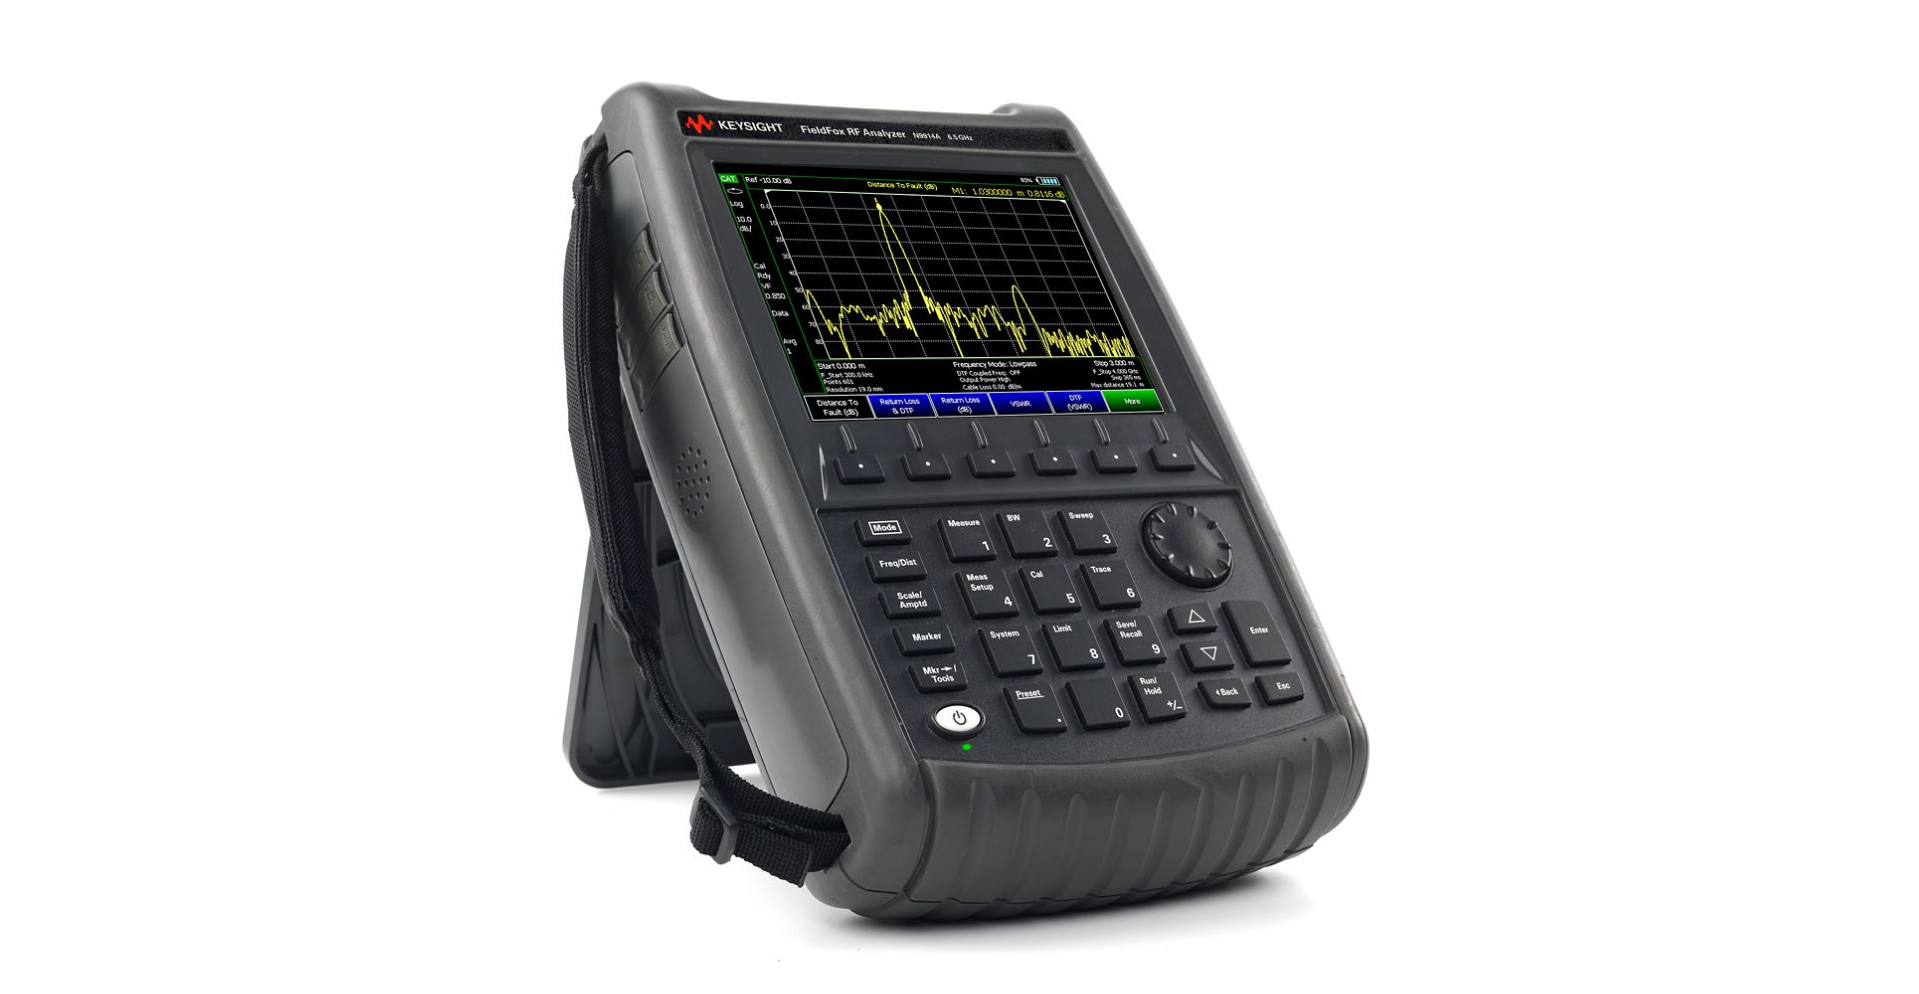
\includegraphics[width=0.4\textwidth]{media/Analyzer.png}
		\caption{N9914A FieldFox Handheld RF Analyzer}
		\label{fig:Analyzer}
	\end{figure}
	
	
	Al realizar la modulación de una señal con una frecuencia de portadora $f_c=86 MHz$, se decidió establecer el ancho de banda para las mediciones, $BW=2MHz$ empezando en 85 MHz hasta 87 MHz.
	
	Para analizar la potencia, al analizador Fielfox permite medir la potencia en el ancho de banda que nosotros queramos, para esto se sigue el siguiente proceso:
	
	\begin{enumerate}
		\item Presionar el botón "Measure"
		
		\begin{figure}[h]
			\centering
			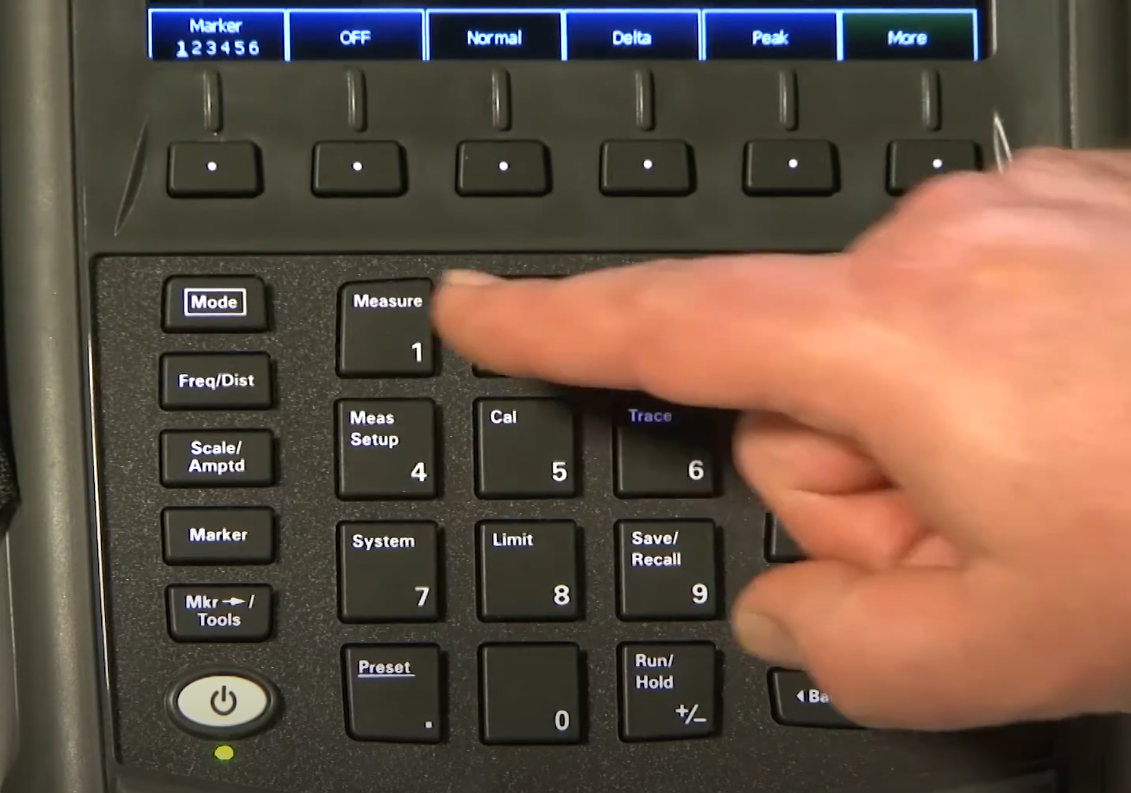
\includegraphics[width=0.8\linewidth]{media/MB.png}
			\caption{Botón "Measure"}
			\label{fig:MB}
		\end{figure}
		
		\item Seleccionar "Channel Measurements"
		
		\begin{figure}[h]
			\centering
			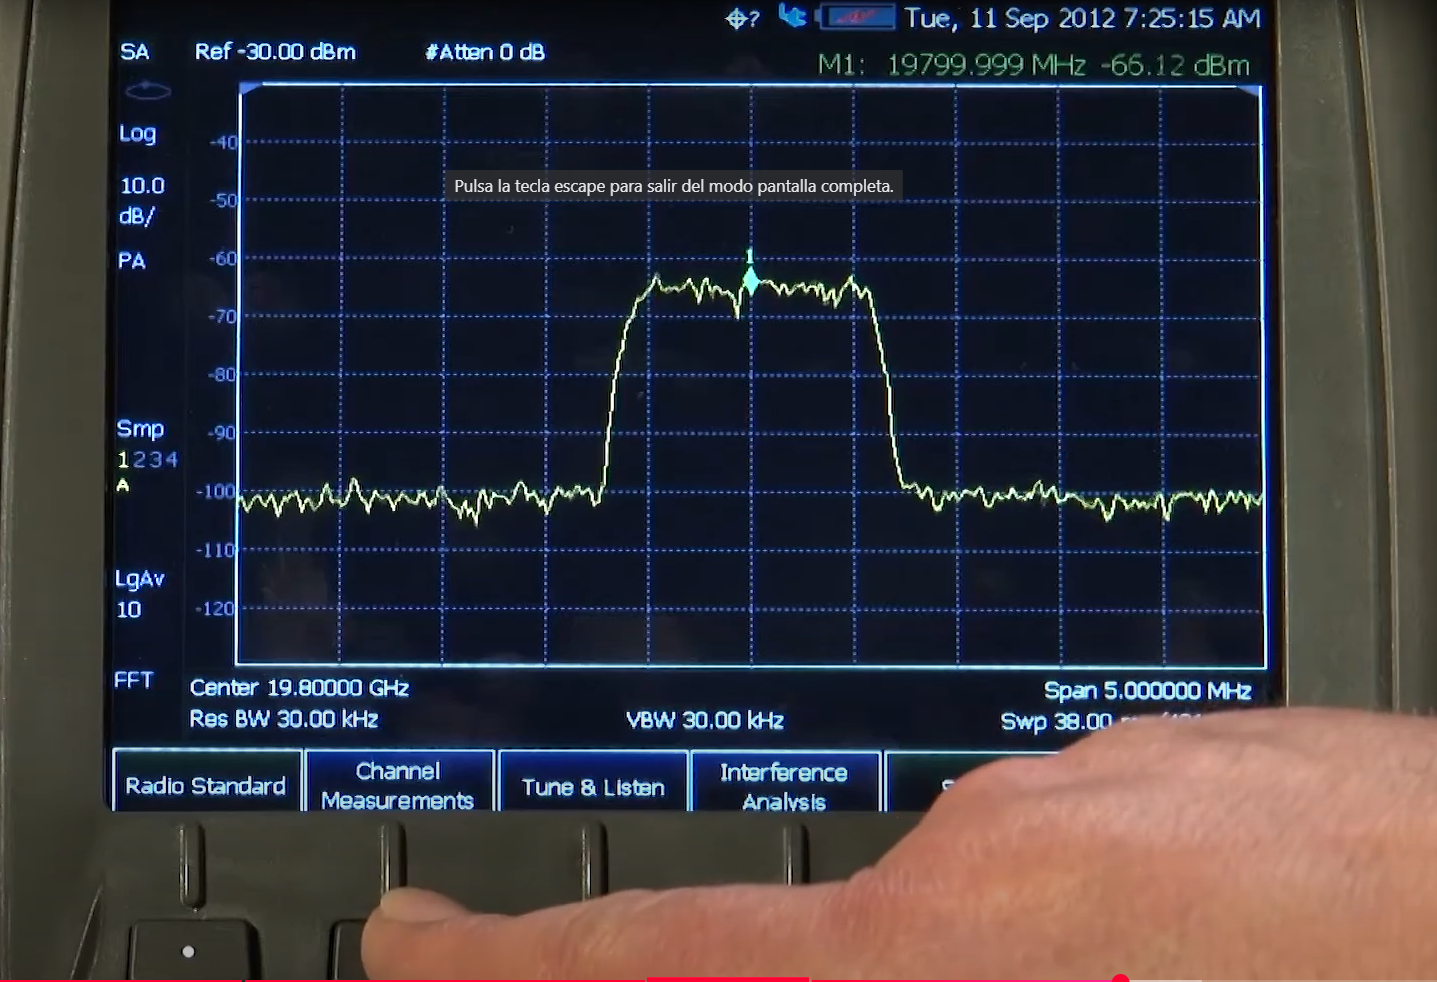
\includegraphics[width=0.8\linewidth]{media/ChMeasB.png}
			\caption{Opción "Channel Measurements"}
			\label{fig:ChMsB}
		\end{figure}
		
		
		\item Seleccionar "Channel Power"
		
		\begin{figure}[h]
			\centering
			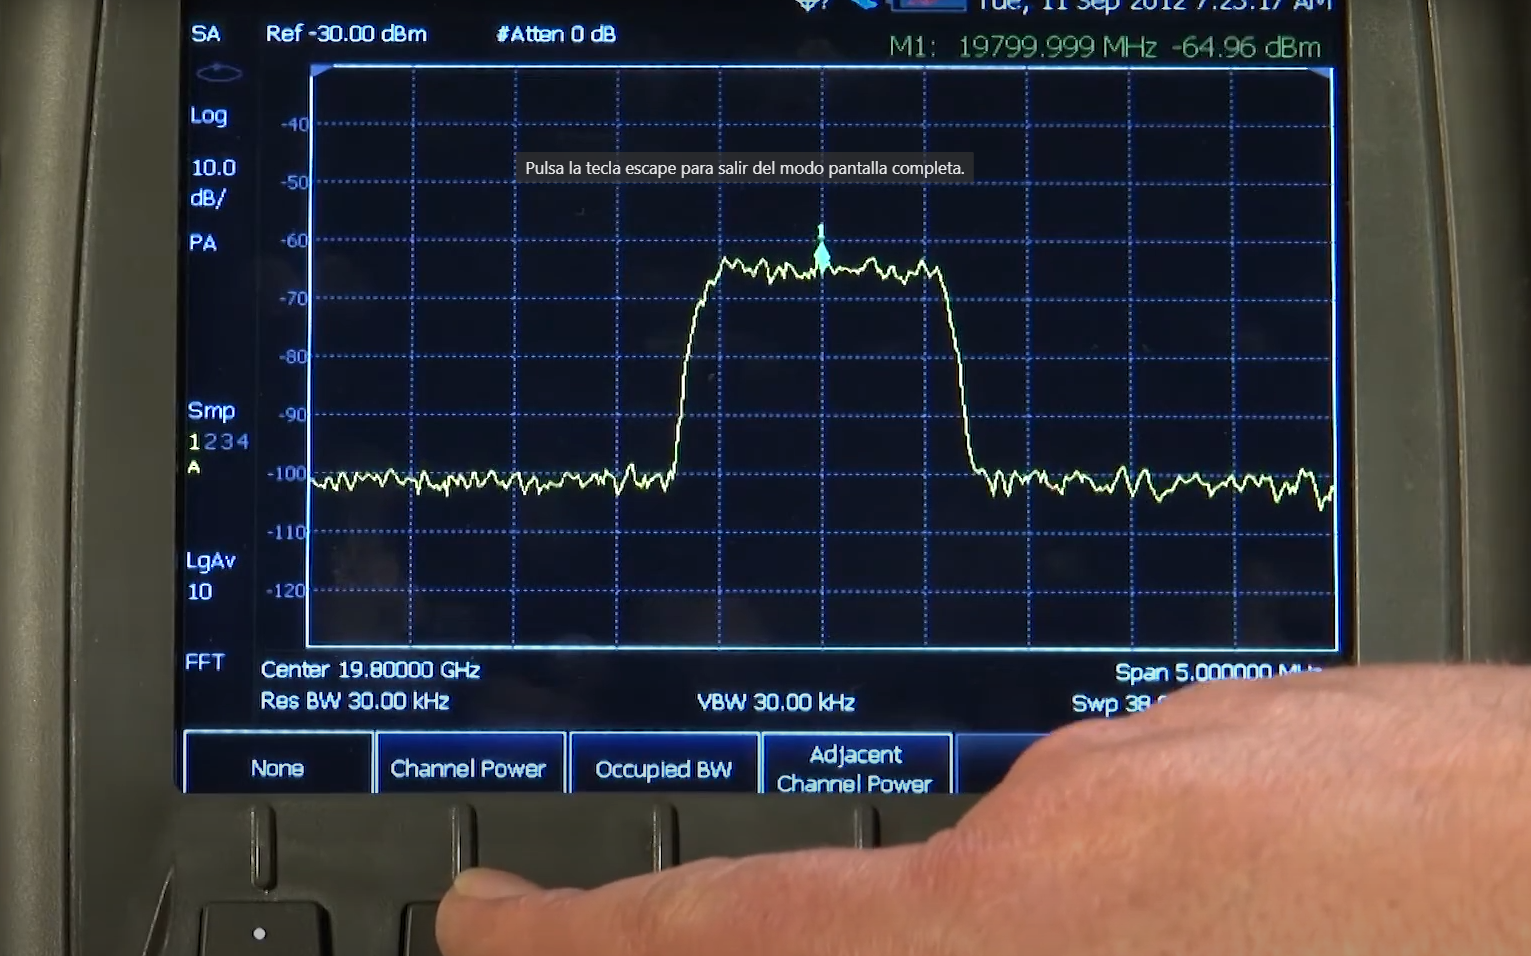
\includegraphics[width=0.8\linewidth]{media/ChPwB.png}
			\caption{Opción "Channel Power"}
			\label{fig:ChPwB}
		\end{figure}
		
		
	\end{enumerate}
	
	Al configurar de esta forma se puede obtener la potencia en el ancho de banda deseado y la densidad espectral de potencia.
	
	\begin{figure}[h]
		\centering
		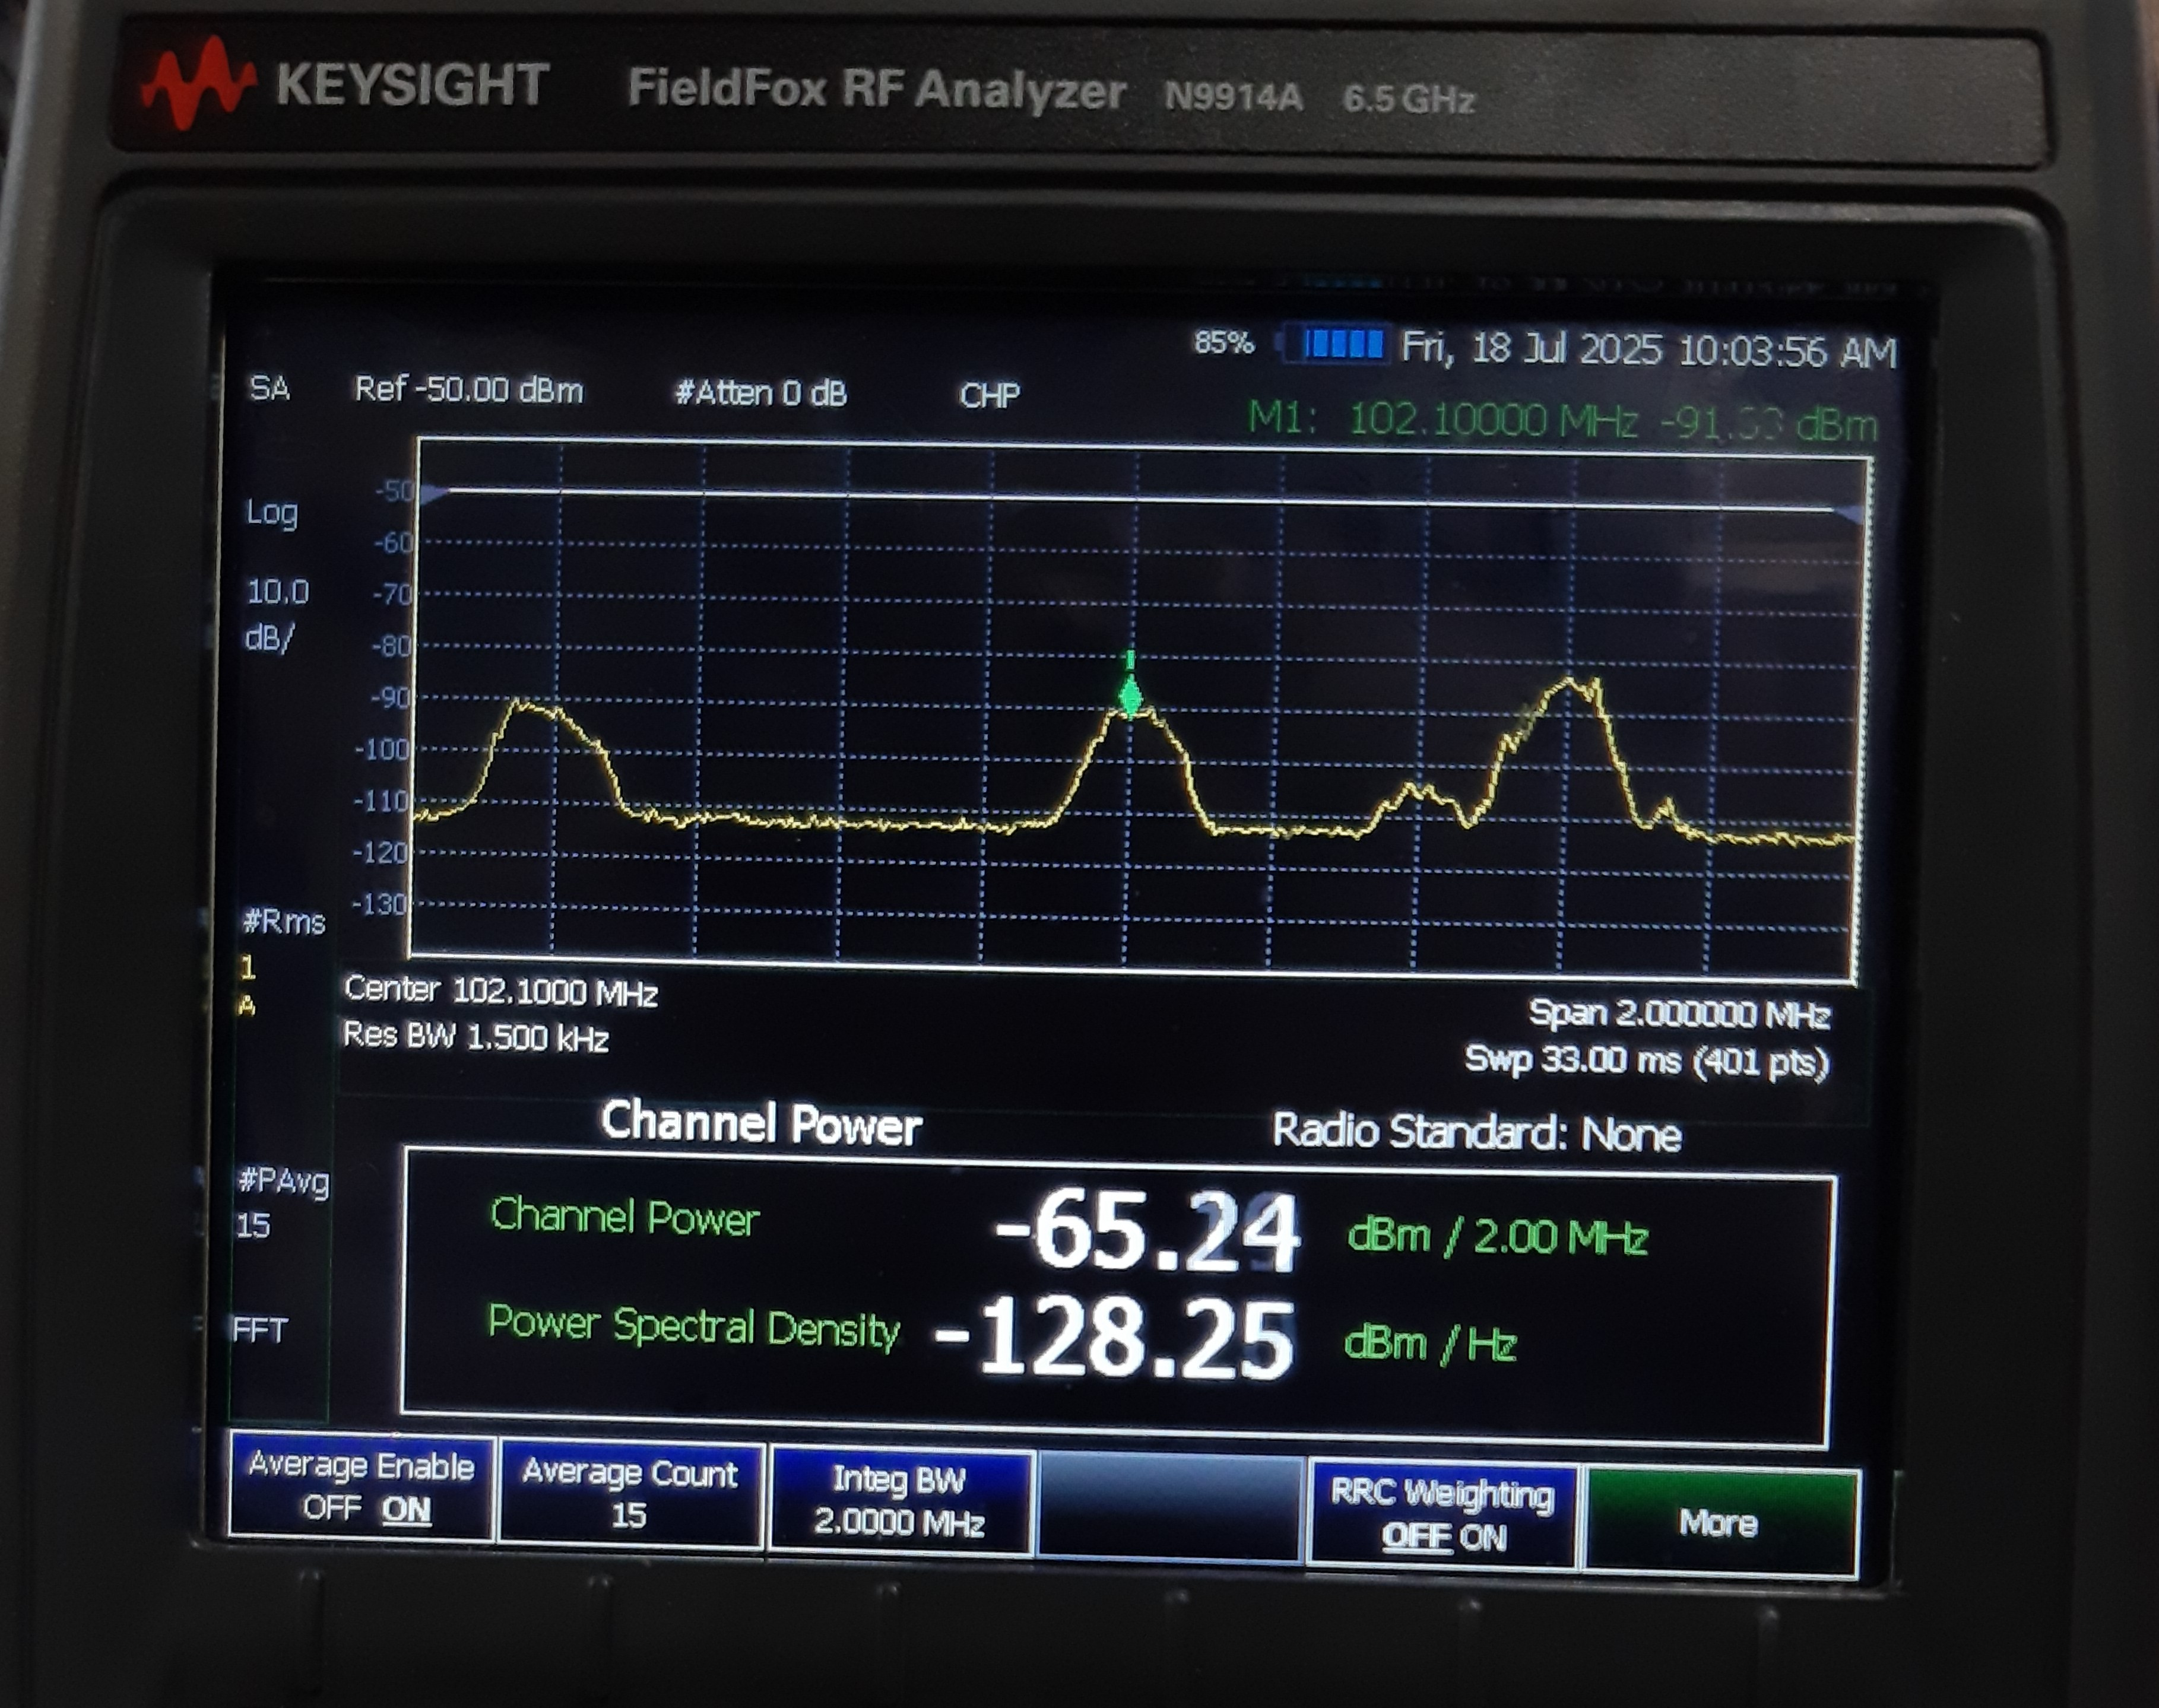
\includegraphics[width=0.8\linewidth]{media/InsConf.jpg}
		\caption{Instrumento configurado para la medición de potencia.}
		\label{fig:InsConf}
	\end{figure}
	
	Una vez configurado el instrumento de medición, se realizaron las mediciones correspondientes, estas se observan en el Anexo A, B y C.
	
	Además de esto, se guardaron los datos de cada medición siguiendo los siguientes pasos:
	
	\begin{enumerate}
		\item Se insertó una unidad de almacenamiento (Tarjeta SD) al instrumento de medición
		\item Presionar el botón "Run/Hold" para pausar la medición
		\item Presionar el botón "Save"
		\item En la opción "Device" escoger la Trajeta SD como almacenamiento
		\item En la opción "File type" escoger el formato deseado, en este caso CSV
		\item Escoger la opción "Save"
		\item Escoger el nombre del archivo a guardar.
	\end{enumerate}
	
	De esta forma se obtuvieron los datos para su posterior análisis.
	
	
	\section{Análisis de datos}
	
	\subsection{ Estimación del piso de ruido }
	
	Para el procesamiento de las mediciones obtenidos en formato .csv, se hizo uso del entorno matricial MATLAB, esto debido a su facilidad para el tratamiento de datos en forma de arreglos y al contar con herramientas de navegación entre directorios, permitió automatizar la lectura, tratado y modificación de los datos medidos.
	
	Para tener una coherencia entre el tratado de datos y los resultados obtenidos, fue necesario categorizar mediante una etiqueta y/o nombre de archivo (cada medición) ello con la finalidad de especificar una determinada distancia, tipo de medición y parámetros configurados en la transmisión FM, para ello se uso:
	
	\begin{itemize}
		\item R[distancia en metros]: Para referirse a una señal compuesta solo por ruido.
		\item SR[consonante][distancia]\_Beta: Define una señal FM transmitida con ruido para un beta determinado.
		\item TPR: Refiere al piso de ruido sin ninguna interferencia provocada.
	\end{itemize}
	
	En la figura \ref{fig:jerarquia-archivos} se puede apreciar el esquema general y la jerarquía de archivos resultante para el procesamiento.
	
	\begin{figure}[h]
		\centering
		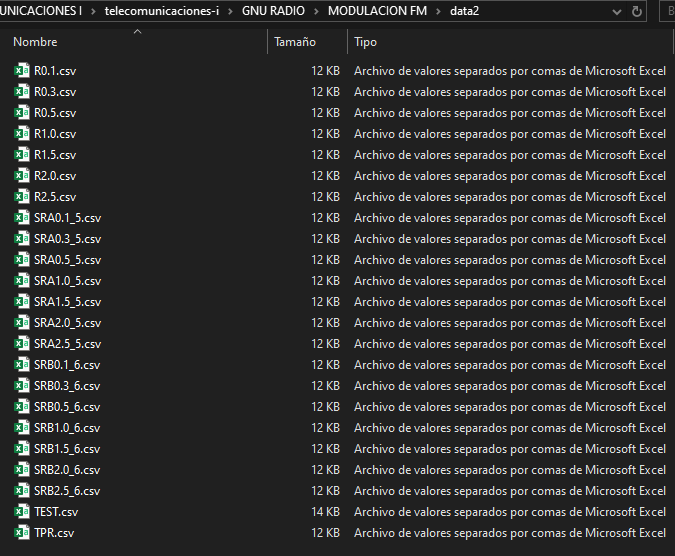
\includegraphics[width=0.5\textwidth]{media/jerarquia-archivos}
		\caption{Jerarquía de Archivo - Procesamiento}
		\label{fig:jerarquia-archivos}
	\end{figure}
	
	
	El piso de ruido esta compuesto por diferentes señales que perturban su medición, como se muestra en la figura \ref{fig:piso-ruido} esta parámetro es de carácter no determinista siendo así que obtener un valor directo es inexacto, por lo que se empleo la obtención de la media entre los valores medidos para obtener un valor representativo que nos permita cuantificar, sin embargo la existencia de los picos (valores extremos) alteran esta medida al desplazar el valor de la media, por lo tanto para evitar este inconveniente, se hace uso de una función limitadora de picos, la cual elimina los valores por fuera de un rango especifico, para facilitar las mediciones.
	
	\begin{figure}[h]
		\centering
		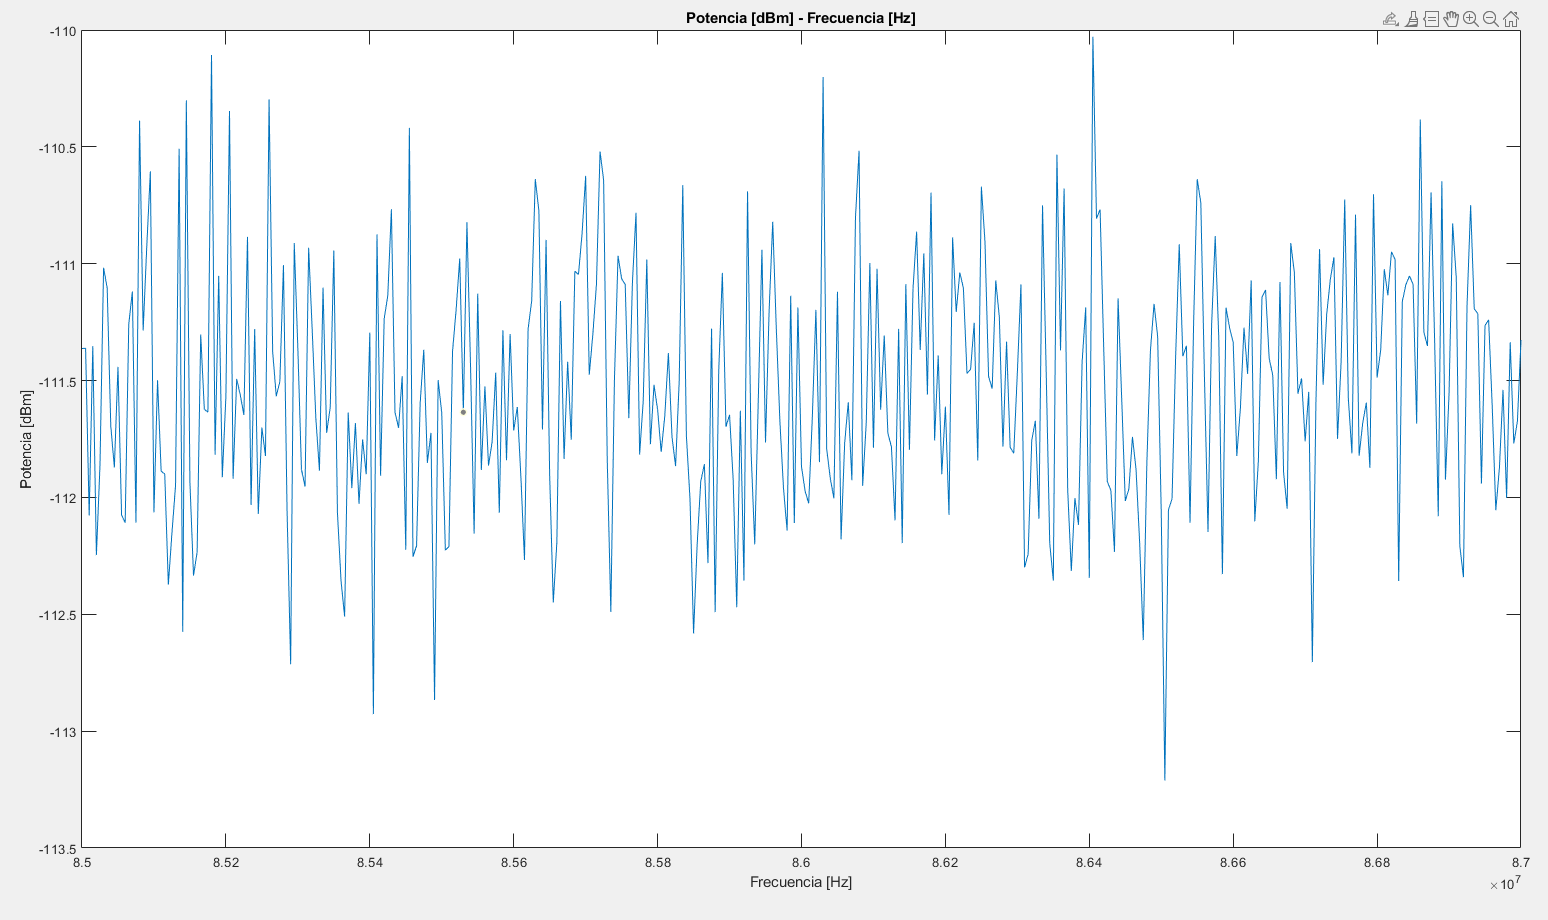
\includegraphics[width=0.5\textwidth]{media/piso-ruido}
		\caption{Piso de Ruido de una señal sin perturbación controlada}
		\label{fig:piso-ruido}
	\end{figure}
	
	Por otro lado en la figura \ref{fig:piso-ruido-disc} se puede apreciar el piso de ruido luego de aplicar un discriminador simple el cual se encargar de suprimir los sobre picos de la señal, para este caso los valores extremos de la señal se ubicaban en la parte inferior de la misma y para valores superiores a los -12dBm, finalmente limitada la señal se obtuvo la media, siendo el piso de ruido equivalente a $-111.5306 [dBm]$
	
	\begin{figure}[h]
		\centering
		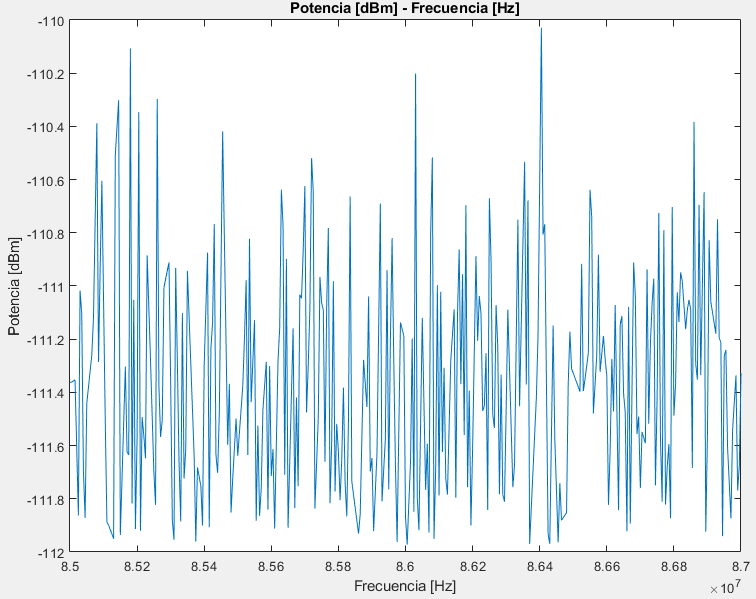
\includegraphics[width=0.5\textwidth]{media/piso-ruido-disc}
		\caption{Piso ruido discriminado}
		\label{fig:piso-ruido-disc}
	\end{figure}
	
	En función al procedimiento para la obtención del piso de ruido este se aplico a las diferentes mediciones realizadas y su archivo de datos de salida correspondiente, para ello además la jerarquía de archivos definida ayudo con este procedimiento permitiendo analizar en caso se desee solo las señales de ruido (sin transmisión) o las señales transmitida para un determinado valor de índice de modulación $\beta$.
	
	Para este propósito se definió un bucle general con instrucciones para realizar la lectura de archivos desde la carpeta $'/data2/'$, seguidamente se realiza el ploteo de las archivos leídos y la media del nivel de ruido obtenido para cada archivo luego de aplicar el discriminador de picos.
	
	En la figura \ref{fig:seniales-ruido} se muestran un gráfica general del piso del ruido siendo afectado por el generador de ruido para las distancias entre $0cm y 250cm$, gráficas que además se tomaron como referencia para establecer un nivel umbral para el discriminador a aplicar.
	
	\begin{figure}[h]
		\centering
		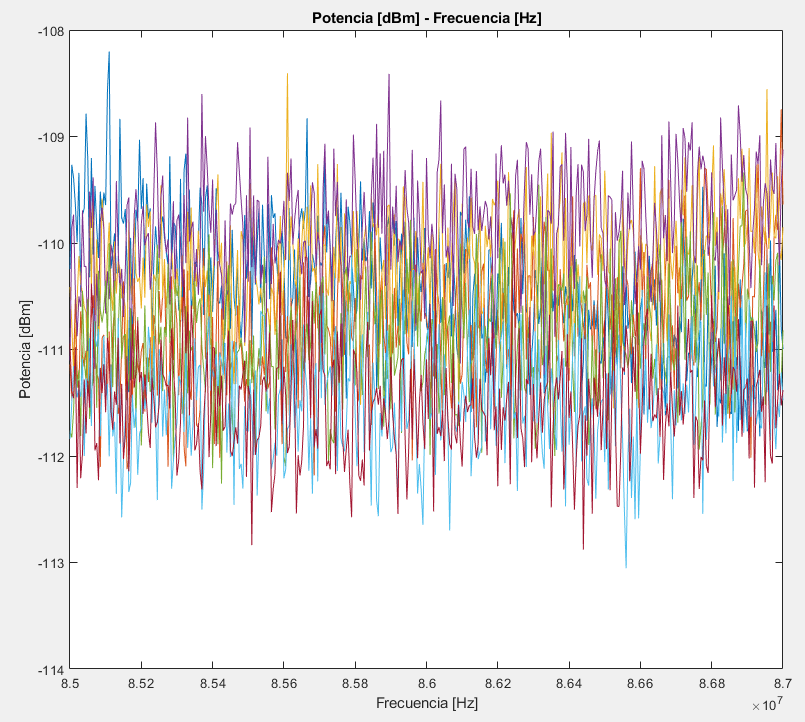
\includegraphics[width=0.5\textwidth]{media/seniales-ruido}
		\caption{Señales de ruido sin transmisión}
		\label{fig:seniales-ruido}
	\end{figure}
	
	Como resultado de este análisis se pudo apreciar que el nivel de ruido presenta sobre picos por debajo de los $-112 [dBm]$, una vez realizadas ambas acciones se ejecutaron 2 procesos por cada ciclo del bucle.
	
	\begin{enumerate}
		\item Eliminar sobrepicos mediante el discriminador
		\item Obtener la media para la señal de ruido a la salida del discriminador.
	\end{enumerate}
	
	Además al mismo tiempo se realiza una correlación entre cada media o promedio resultante con la distancia del generador de ruido al analizador de espectros con el cual se realizaron las medidas, siendo así que el primer punto y consecuentes se correlacionan con las medidas en distancia de $10, 30, 50, 100, 150, 200, 250$ cm para cada una de ellas respectivamente, el resultado de este procedimiento se puede apreciar en la figura \ref{fig:potencia-distancia}.
	
	\begin{figure}[h]
		\centering
		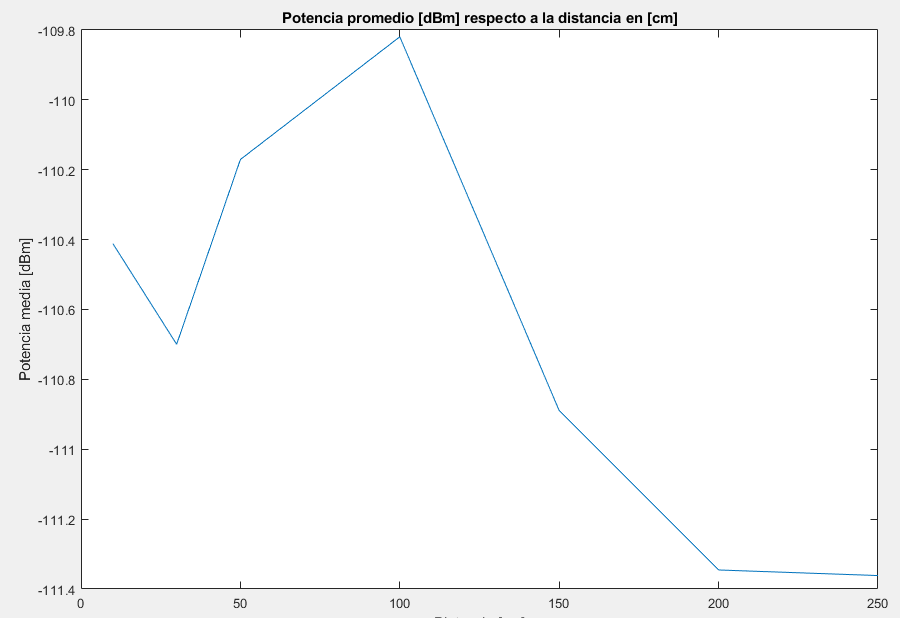
\includegraphics[width=0.5\textwidth]{media/potencia-distancia}
		\caption{Piso de ruido respecto al nivel a la distancia del generador de ruido}
		\label{fig:potencia-distancia}
	\end{figure}
	
	En la tabla \ref{tab:resumen-piso-ruido} se muestra una tabla resumen de las media obtenido para cada medición en función a la distancia.
	
	\begin{table}
		\centering
		\begin{tabular}{ll}
			\textbf{Distancia {[}cm{]}} & \textbf{Piso de Ruido {[}dBm{]}} \\
			10                          & -110.4115                        \\
			30                          & -110.6997                        \\
			50                          & -110.1706                        \\
			100                         & -109.8195                        \\
			150                         & -110.8894                        \\
			200                         & -111.3456                        \\
			250                         & -111.3615                       
		\end{tabular}
		\caption{Resumen: Distancia respecto al piso de ruido}
		\label{tab:resumen-piso-ruido}
	\end{table}
	
	De lo anterior se puede concluir que a 250 centímetros no existe una afectación relevante en el piso de ruido a causa del generador de ruido cuyo valor de referencia es equivalente a $-111.5306 [dBm]$ mientras que ello se va incrementando conforme la distancia se acorta entre la antena receptora, obteniendo su valor pico a los 100 cm para un valor de $-109.819 [dBm]$
	
	\section{Conclusiones}
	\begin{itemize}
		\item Se lograron implementar los bloques de transmisión y recepción FM para analizar el efecto del ruido durante la recepción
		\item Se logro establecer una correlación entre el nivel de ruido generado y la distancia para una transmisión FM, implicando para ello que en función a las mediciones realizadas
		\item Se estableció a que una distancia de 100cm el efecto de ruido respecto al generador es máximo, lo cual eleva el piso del ruido en $1.542 [dBm]$. 
	\end{itemize}
	
	\section{Observaciones}
	
	\begin{itemize}
		\item El uso de la media como determinante en el nivel de ruido es un proceso que se ve afectado fácilmente por valores extremos (sobre picos en la señal), por lo tanto un método alternativo podría brindar mayor certeza sin la necesidad de aumentar la complejidad computacional.
		\item A pesar de la eficiencia en el sistema de bloques definidos para la transmisión y recepción de la señal FM en GNU Radio es posible mejorar los mismos para poder modificar la mayor cantidad de parámetros como la amplitud de la señal de información, el índice de modulación, frecuencia de corte de los filtros, los cuales actualmente se definen de forma estática.
		\item Se recomienda realizar mediciones espaciadas al efecto del generador de audio ruido, debido a que un uso consecutivo del mismo limita sus efectos lo cual también podría estar sujeto a otras condiciones, estando aun configurado a su máximo nivel de interferencia.
		\item A partir del análisis de datos también es posible determinar el ancho de banda para cada transmisión FM, teniendo en cuenta para ello el indice de modulación $\beta$.
	\end{itemize}
	
	\bibliographystyle{IEEEtran}
	\bibliography{biblio}	
	
	\newpage
	
	\section{Anexos}
	
	\subsection{Anexo A: Mediciones de Ruido puro}
	\begin{figure}[h]
		\centering
		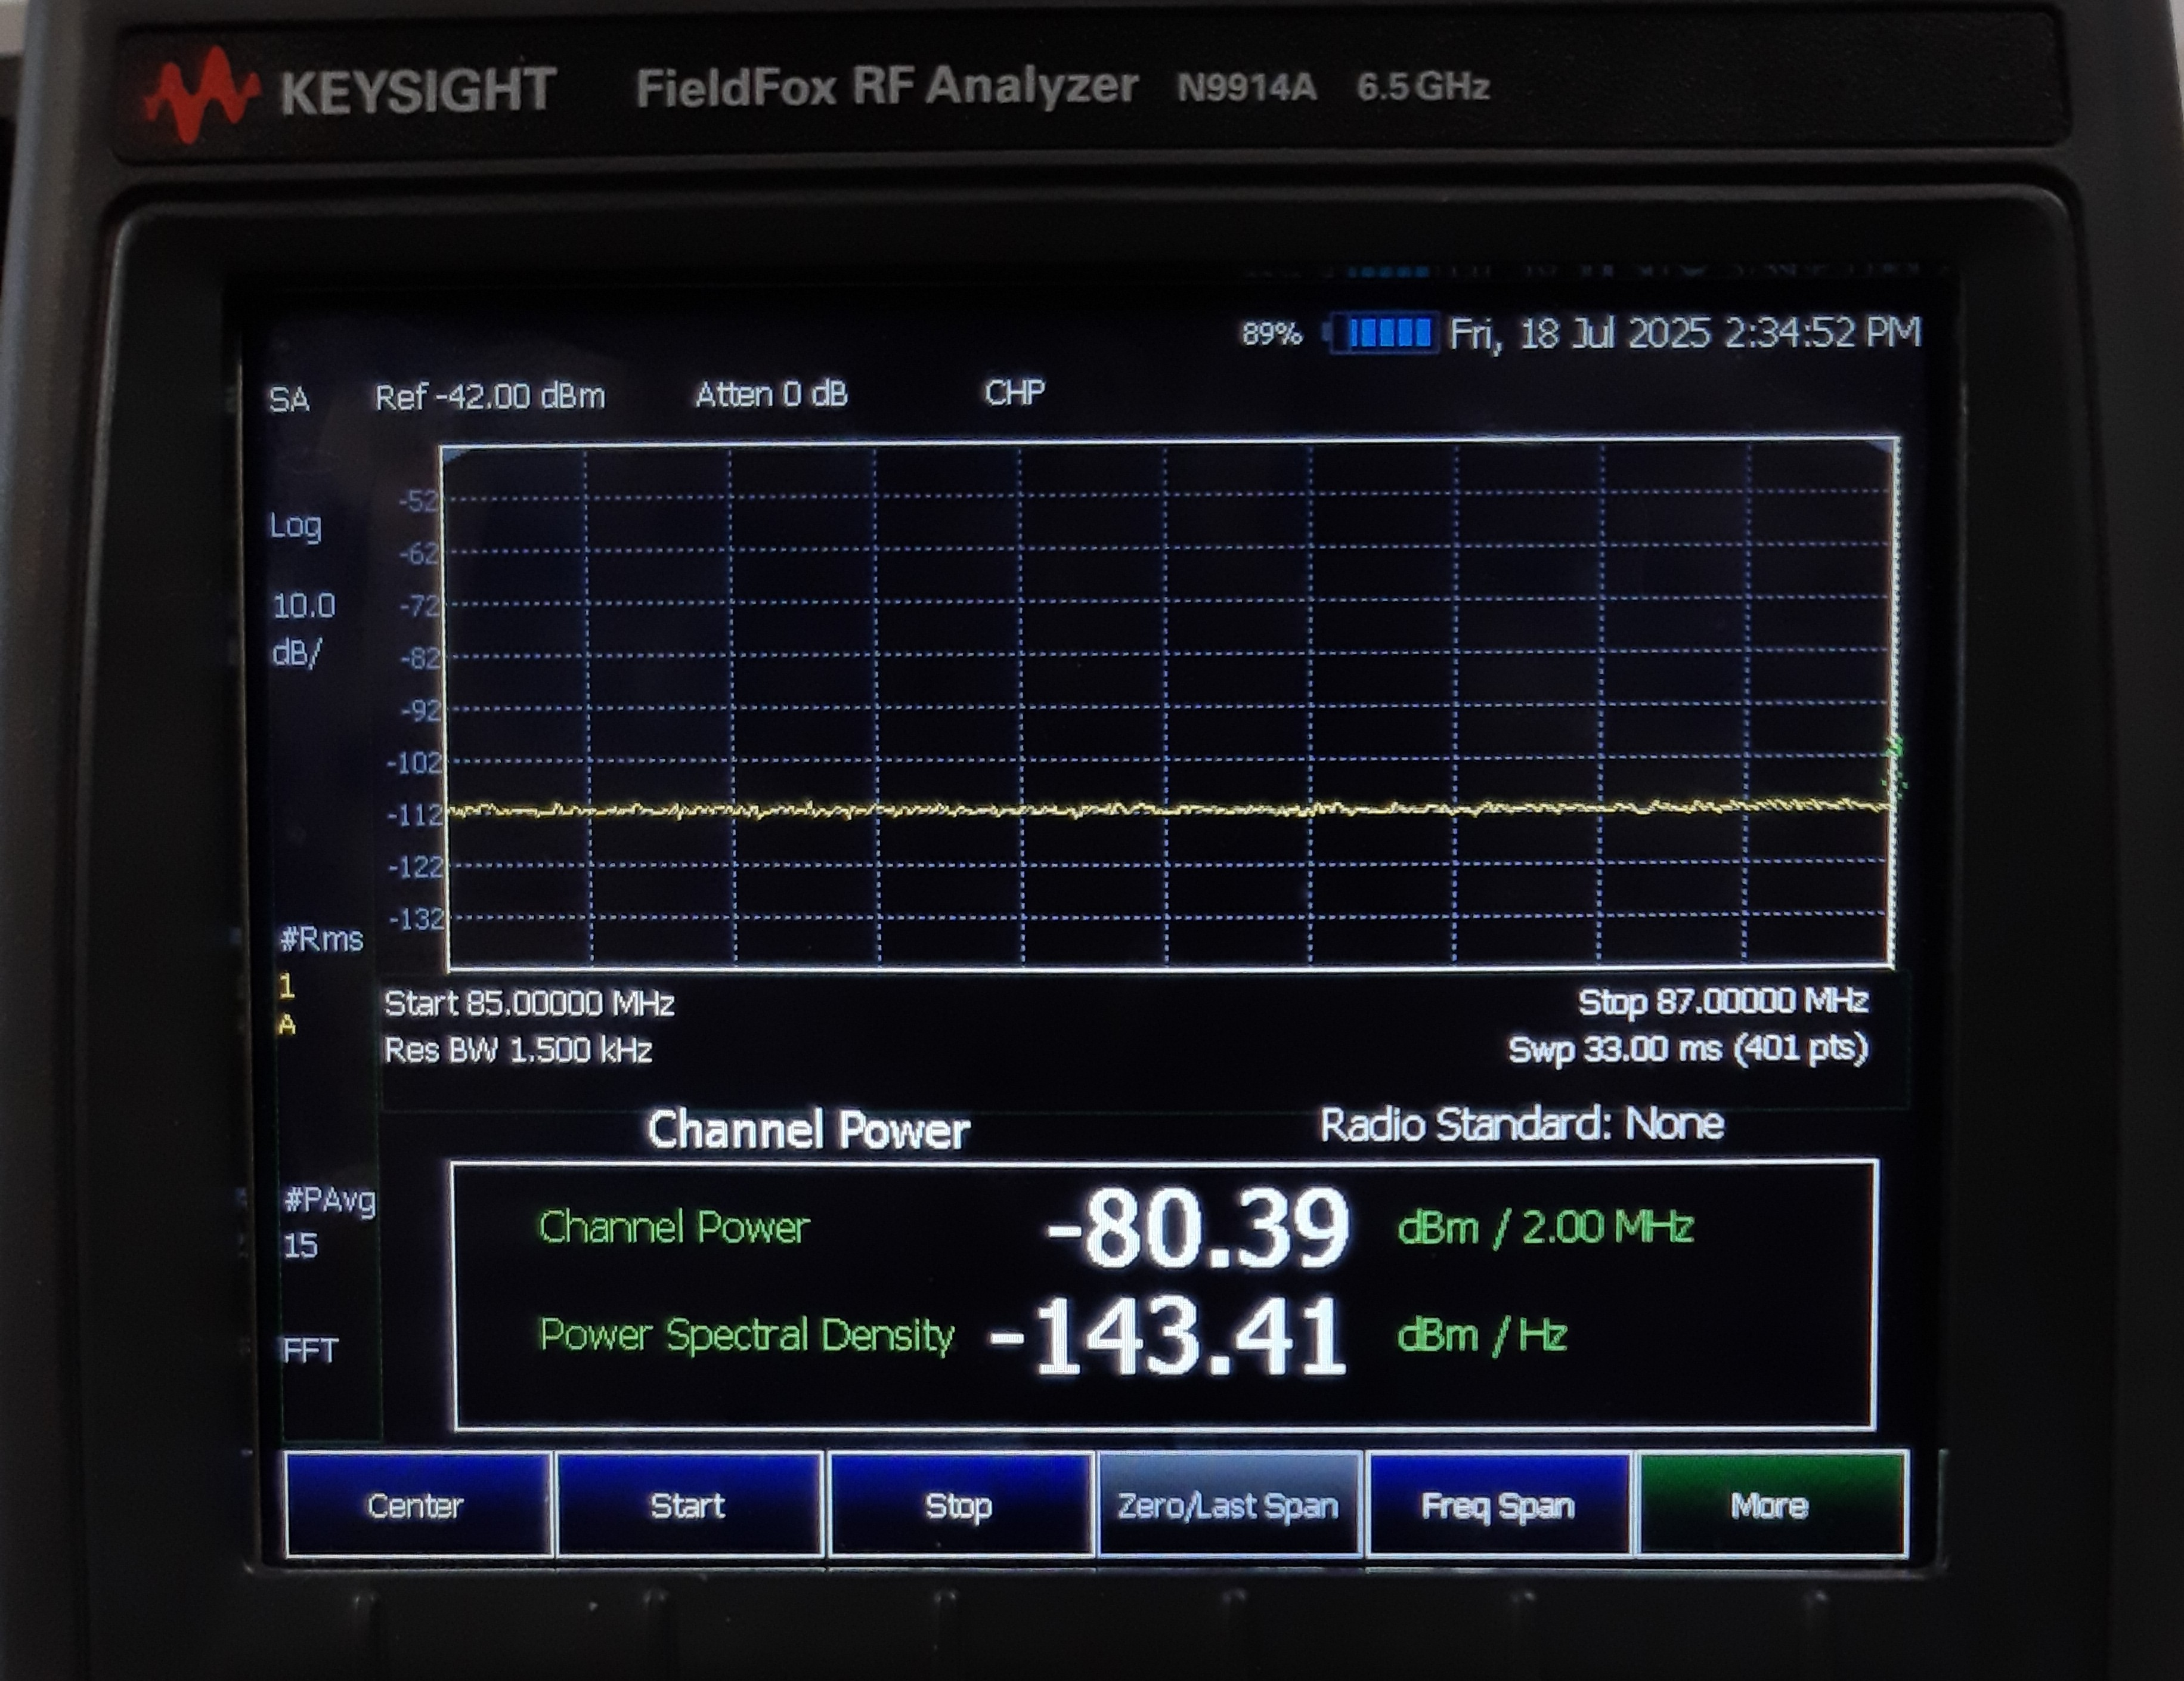
\includegraphics[width=0.4\textwidth]{media/M-PisoRuido.jpg}
		\caption{Medición de potencia de piso de ruido}
		\label{fig:M-PisoRuido}
	\end{figure}
	
	\begin{figure}[h]
		\centering
		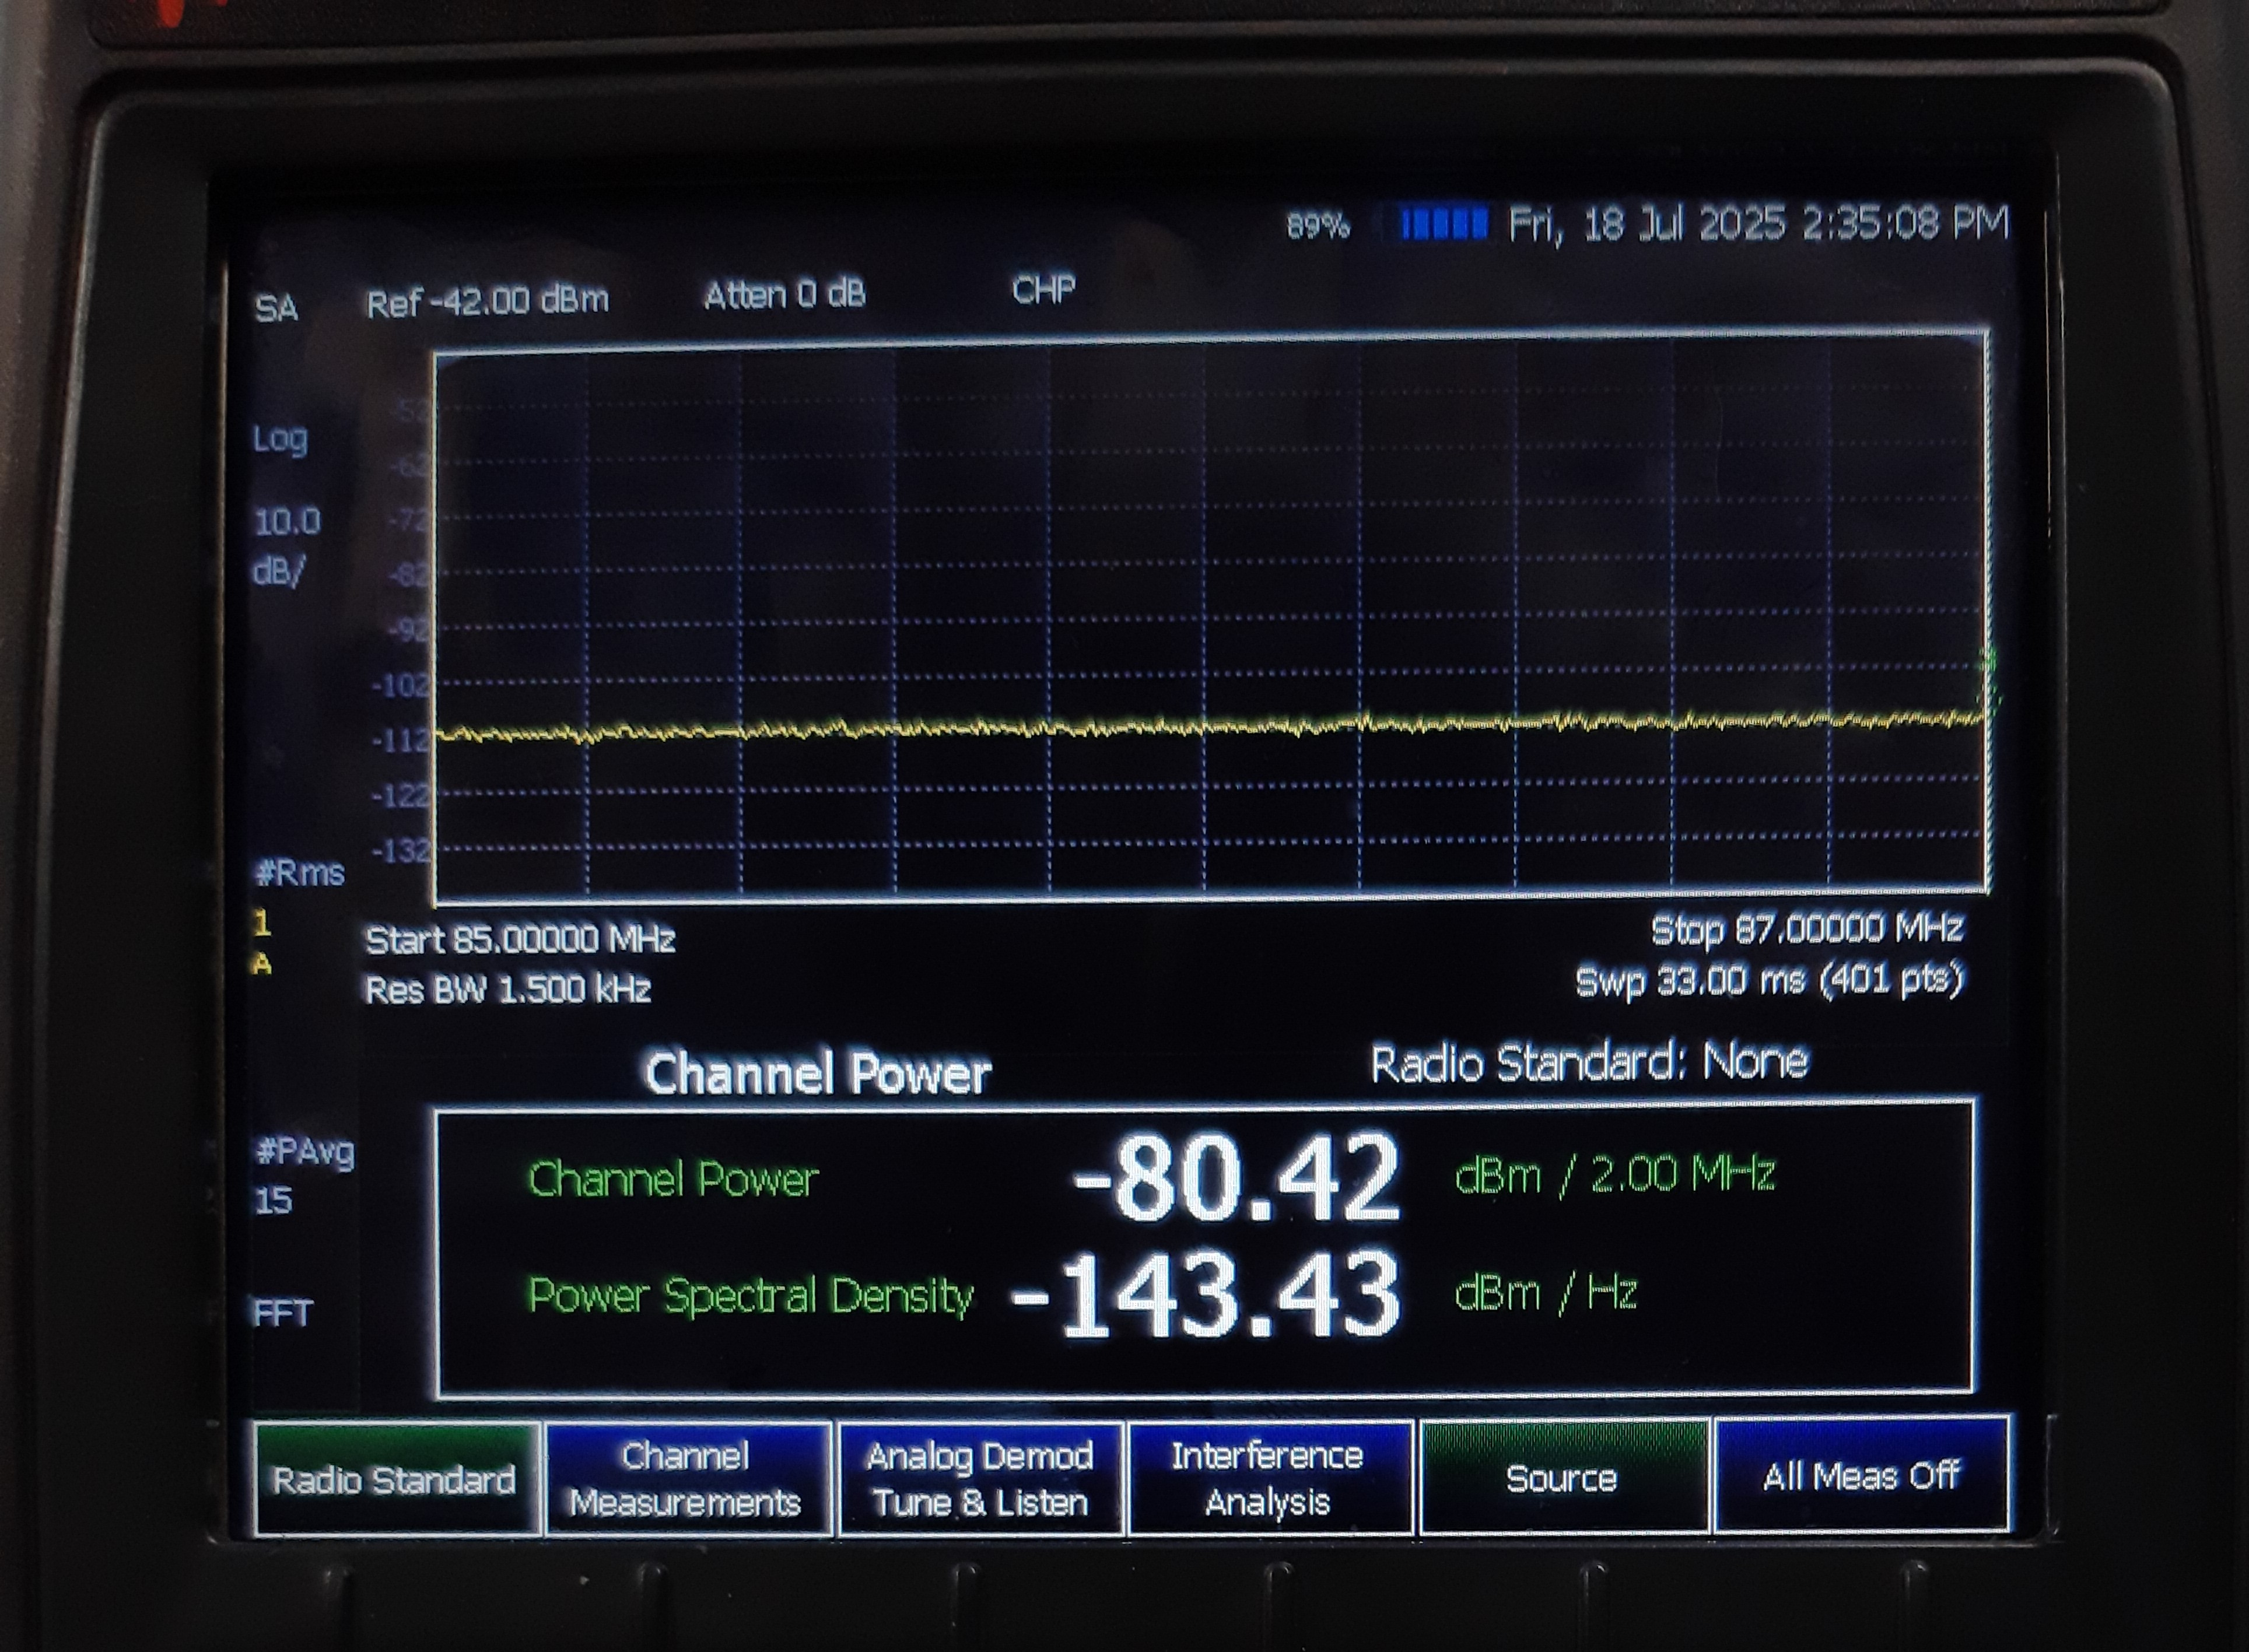
\includegraphics[width=0.4\textwidth]{media/M-Ruido2.5.jpg}
		\caption{Medición de potencia con generador de ruido a 2.5 m}
		\label{fig:M-Ruido2.5}
	\end{figure}
	
	\begin{figure}[h]
		\centering
		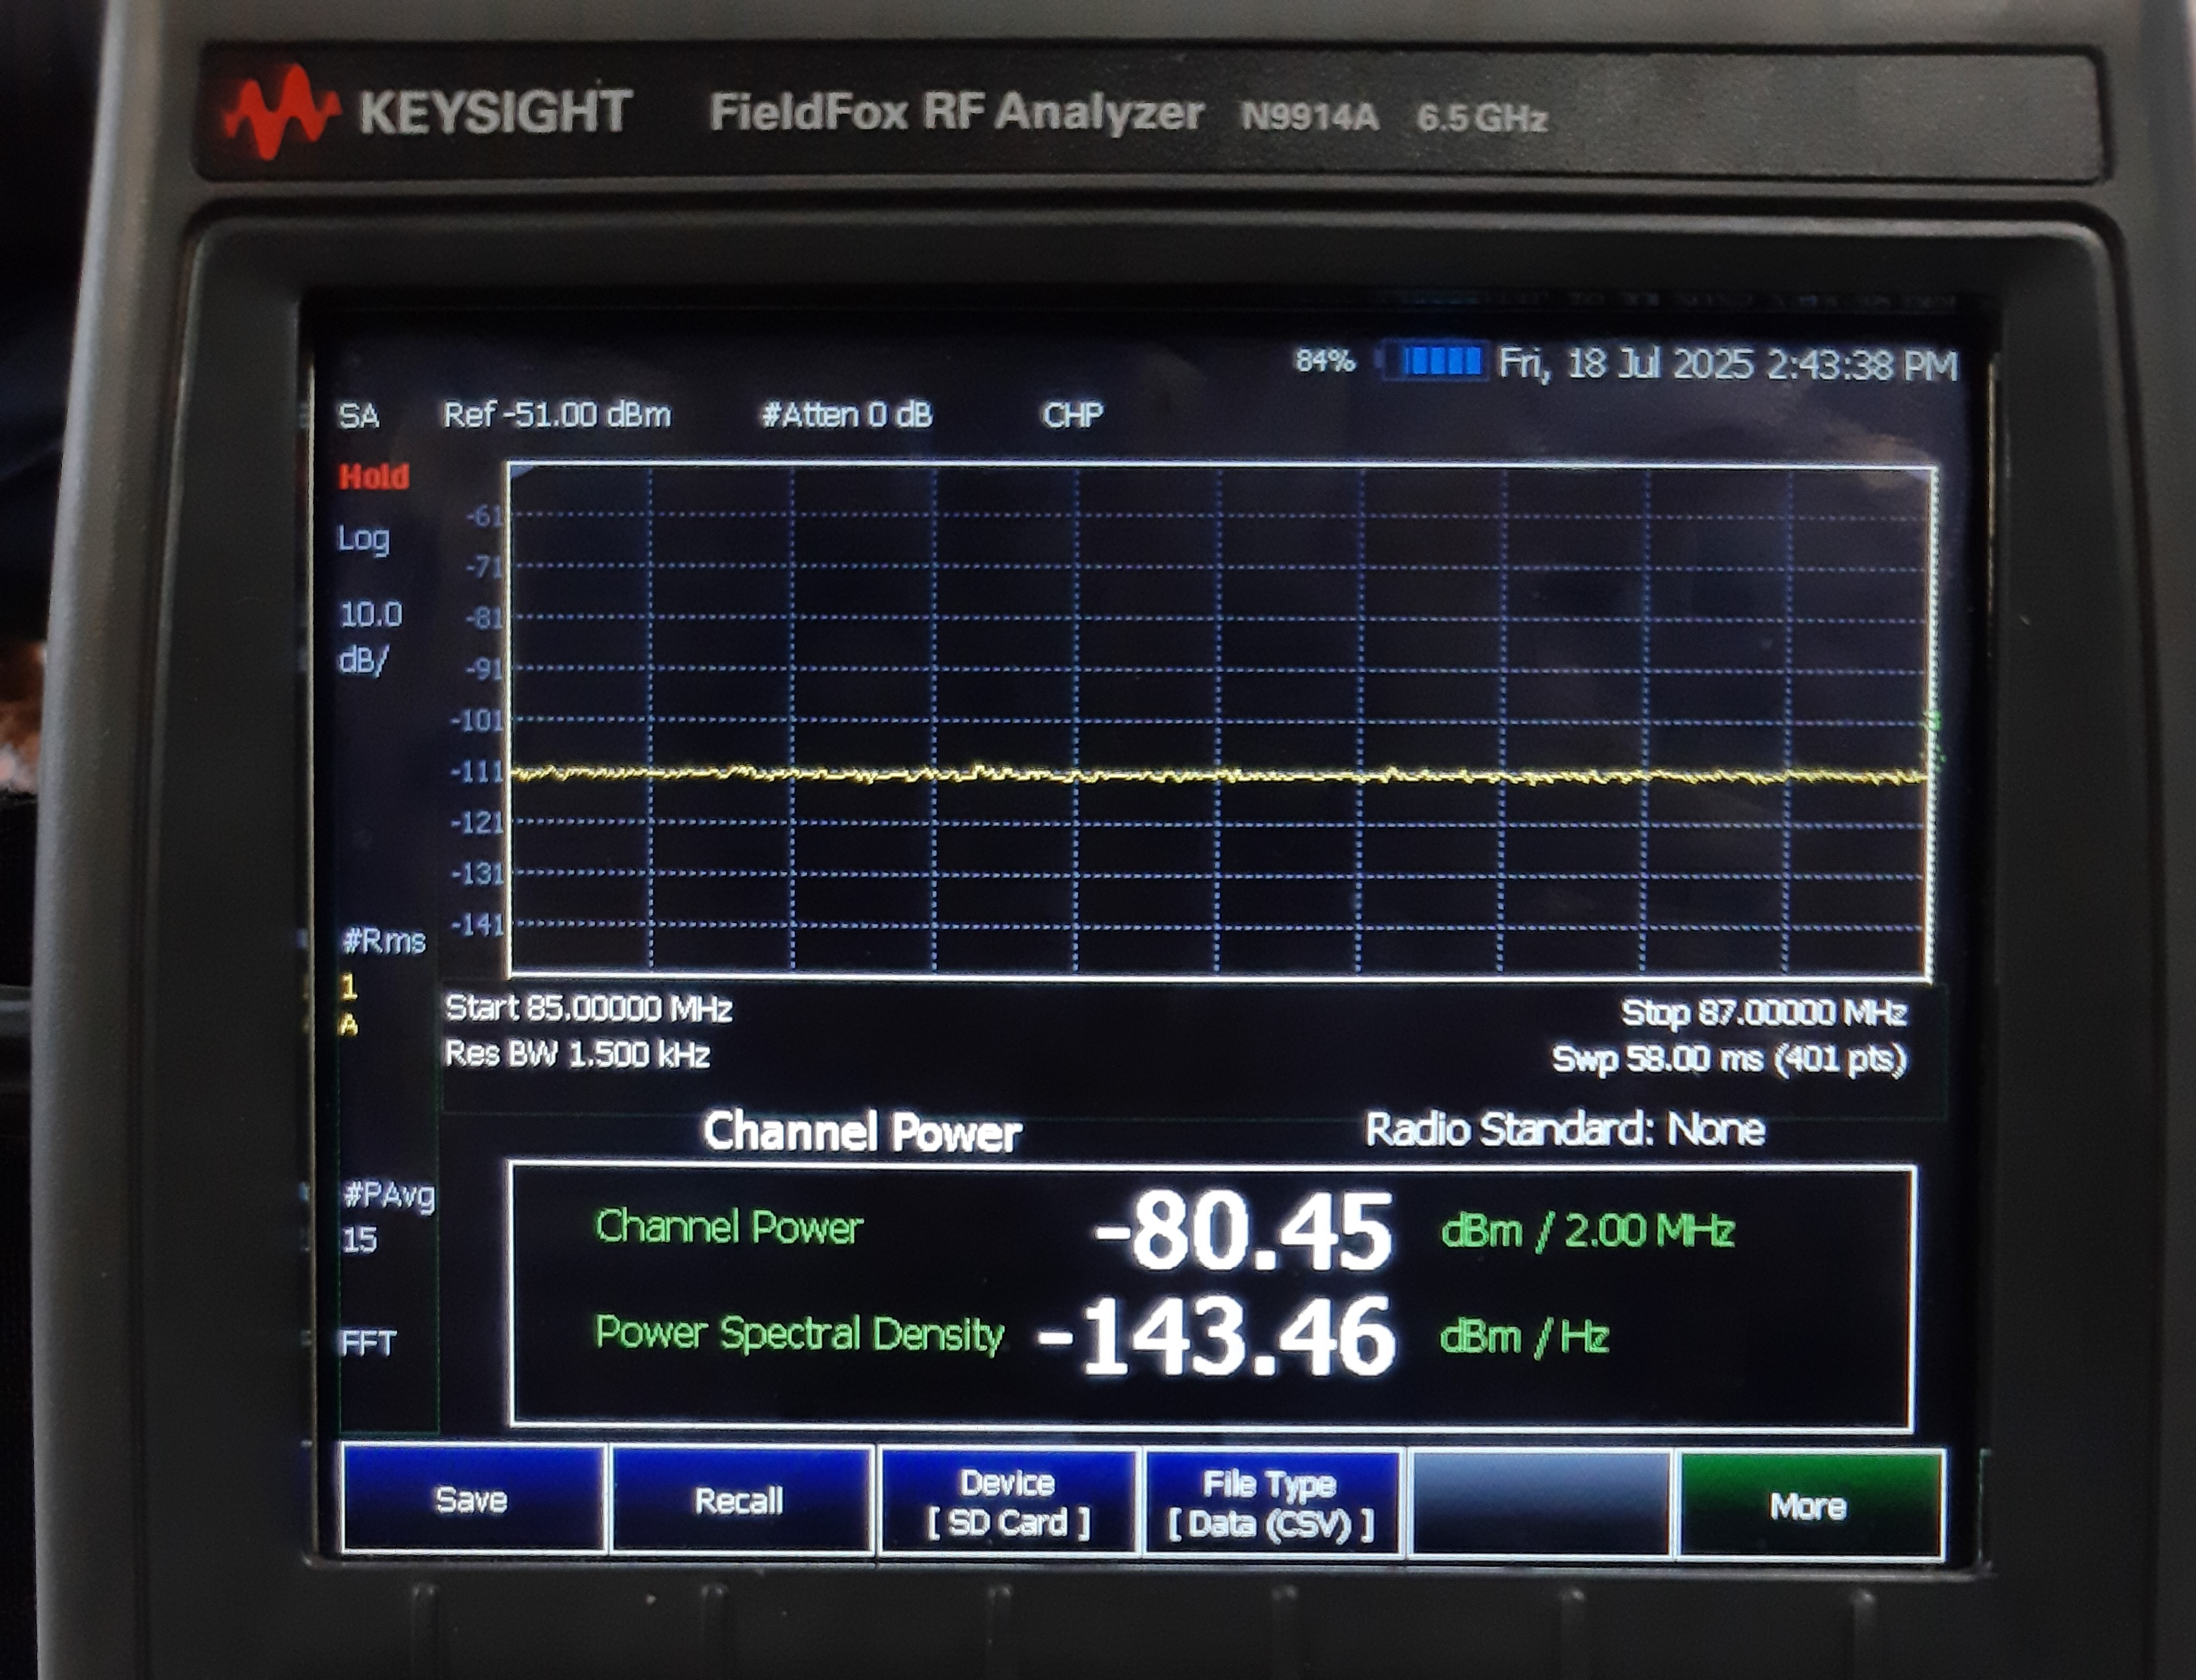
\includegraphics[width=0.4\textwidth]{media/M-Ruido2.jpg}
		\caption{Medición de potencia con generador de ruido a 2 m}
		\label{fig:M-Ruido2}
	\end{figure}
	
	\begin{figure}[h]
		\centering
		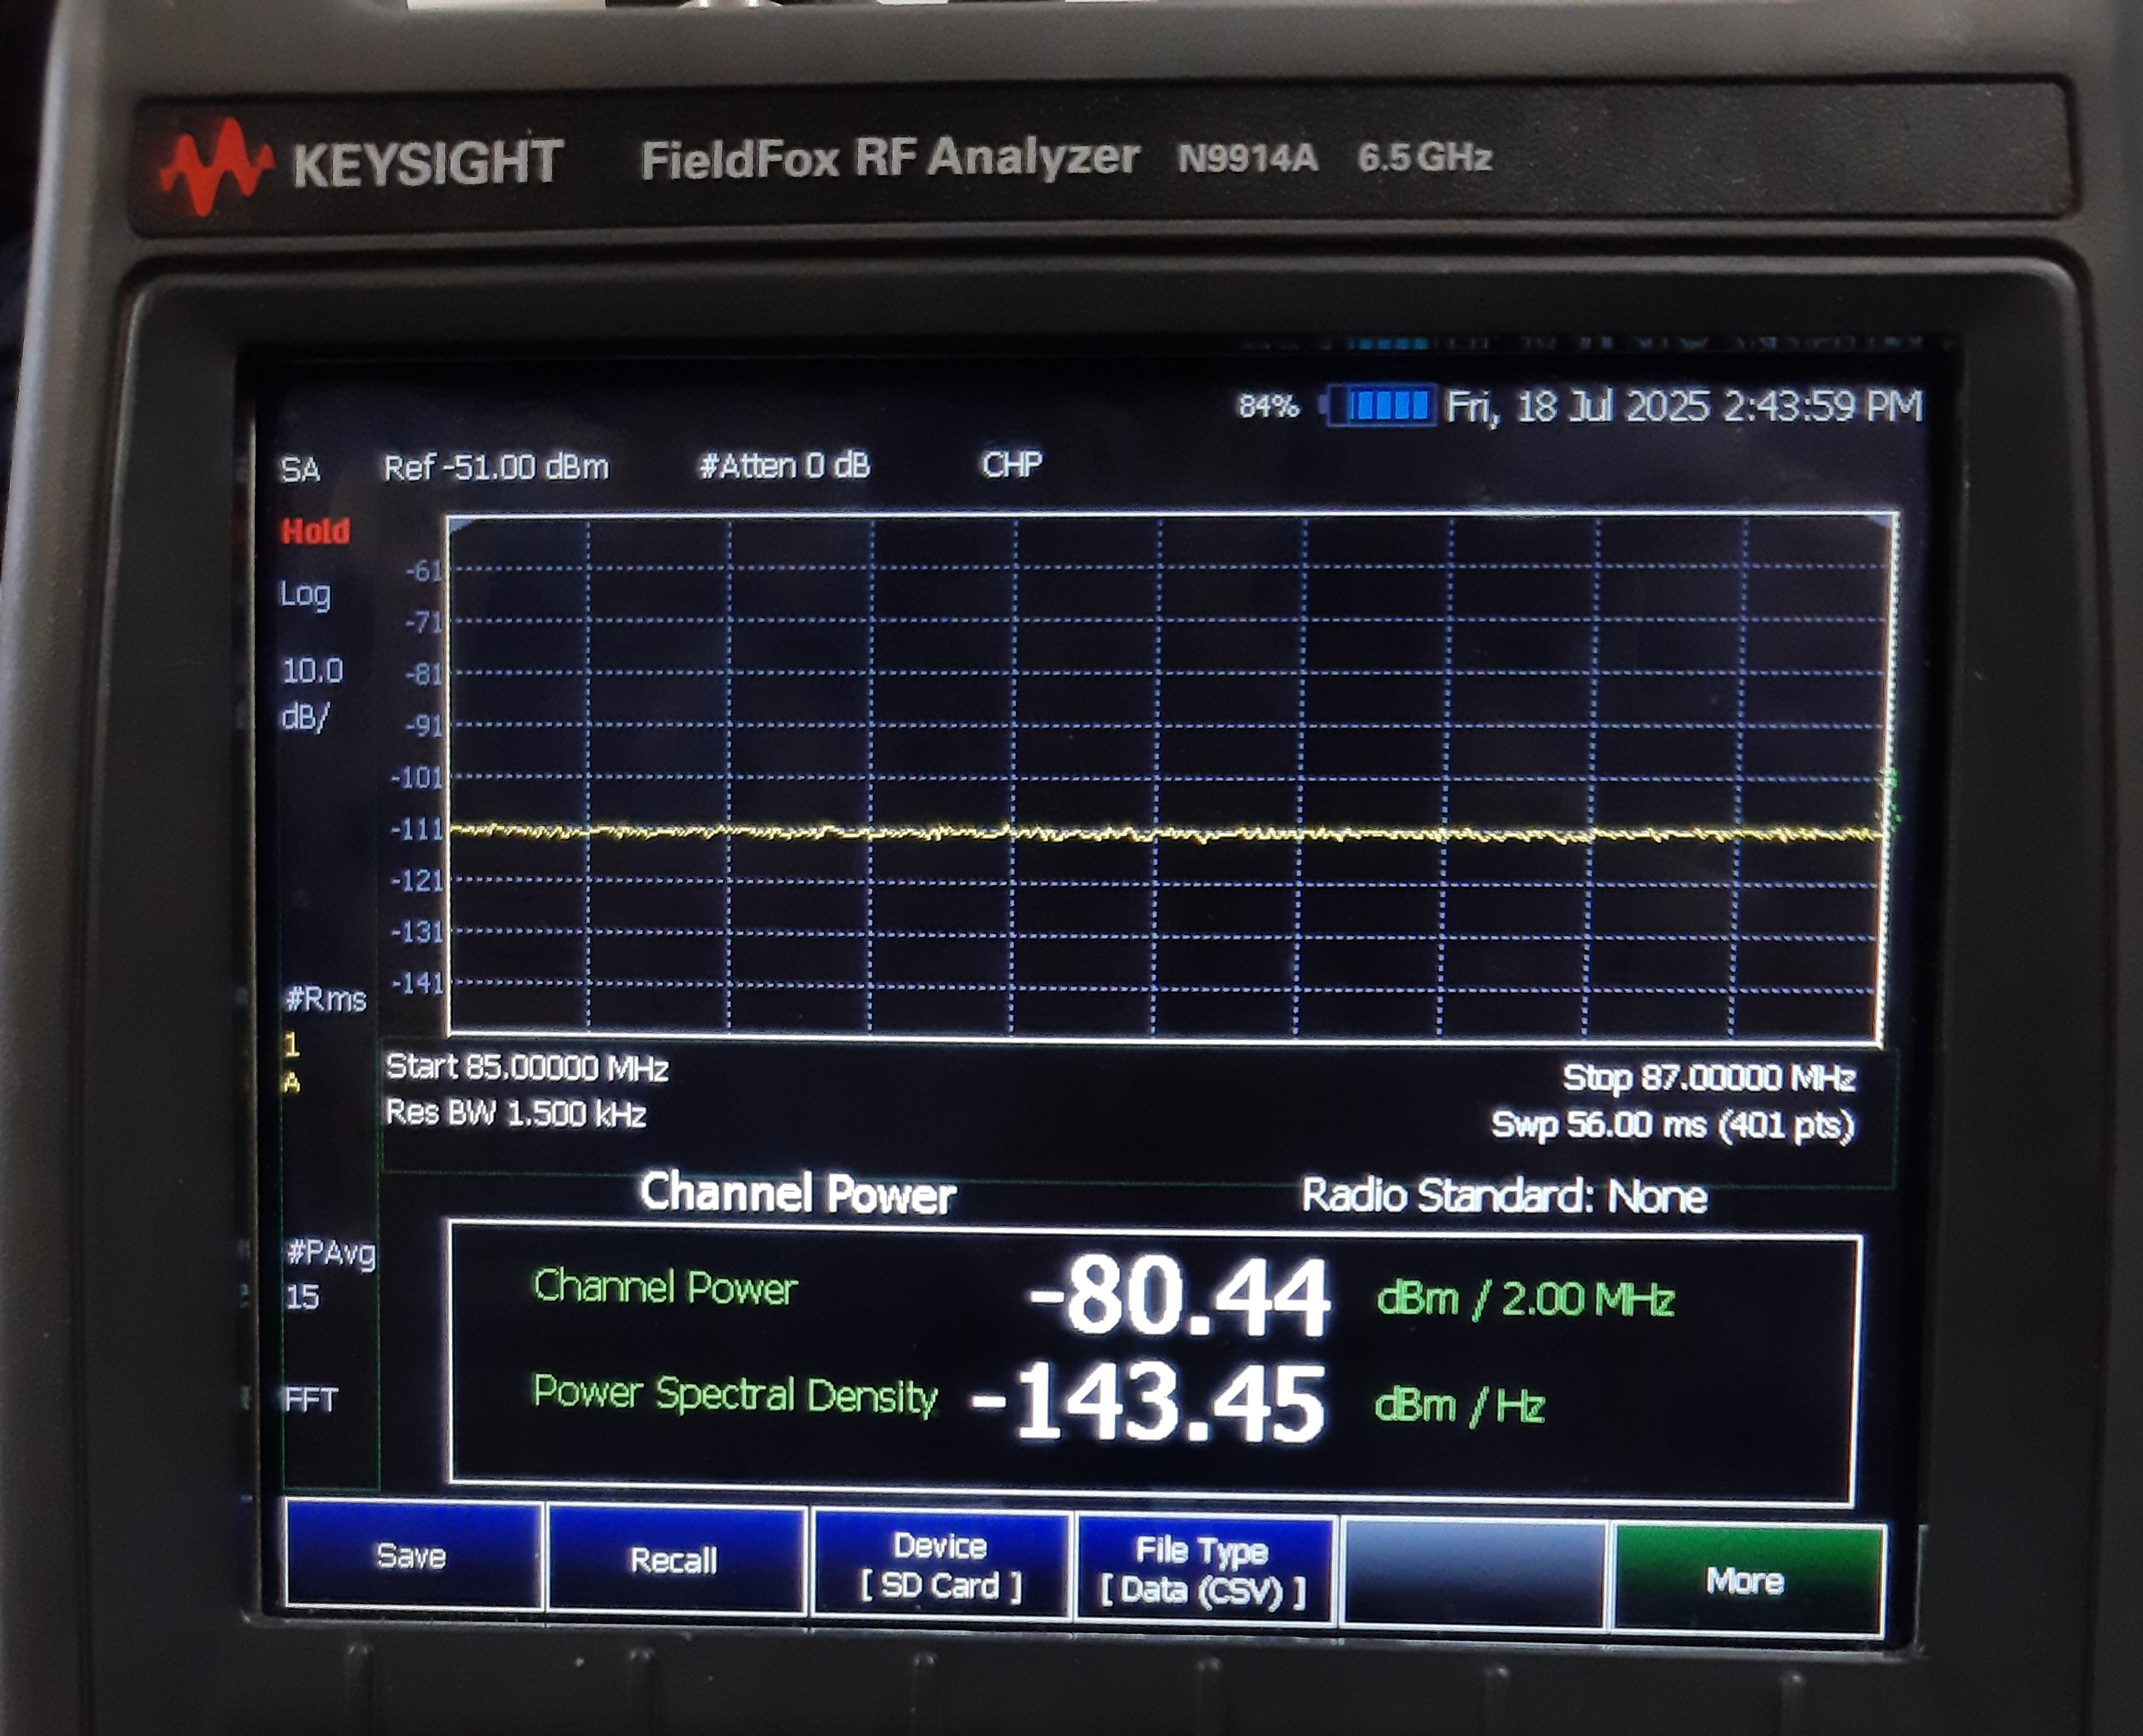
\includegraphics[width=0.4\textwidth]{media/M-Ruido1.5.jpg}
		\caption{Medición de potencia con generador de ruido a 1.5 m}
		\label{fig:M-Ruido1.5}
	\end{figure}
	
	\begin{figure}[h]
		\centering
		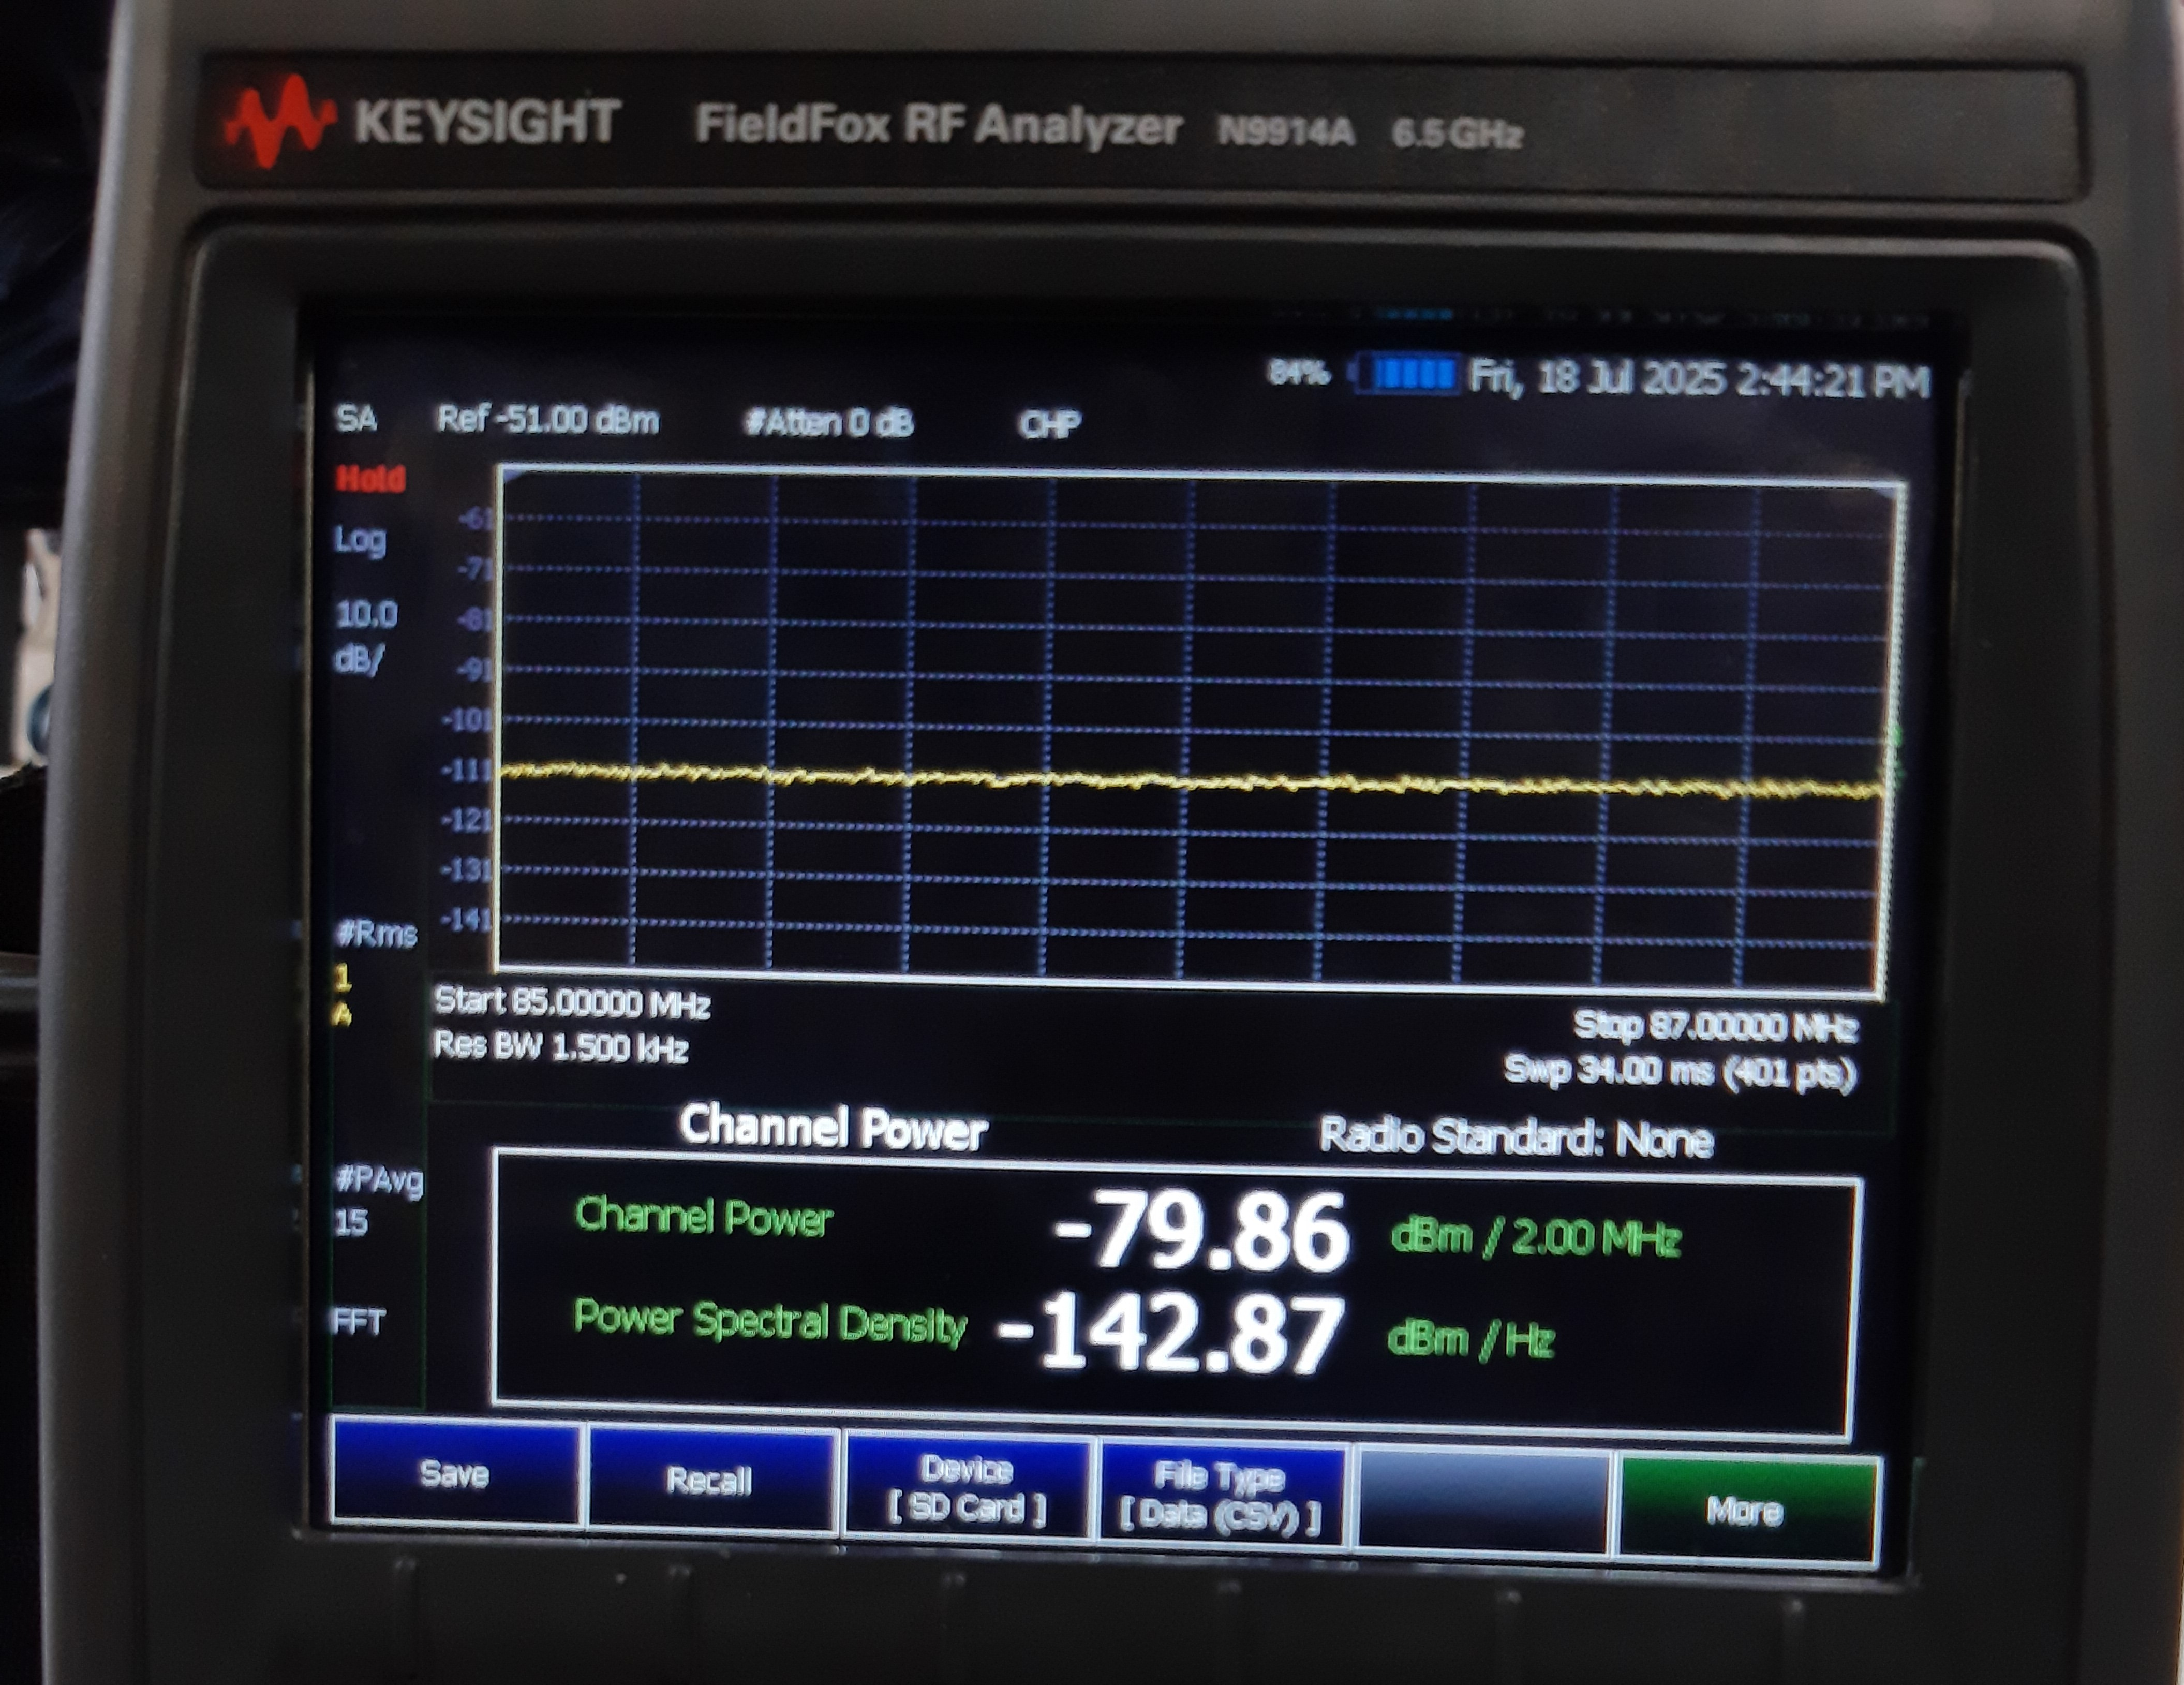
\includegraphics[width=0.4\textwidth]{media/M-Ruido1.jpg}
		\caption{Medición de potencia con generador de ruido a 1 m}
		\label{fig:M-Ruido1}
	\end{figure}
	
	\begin{figure}[h]
		\centering
		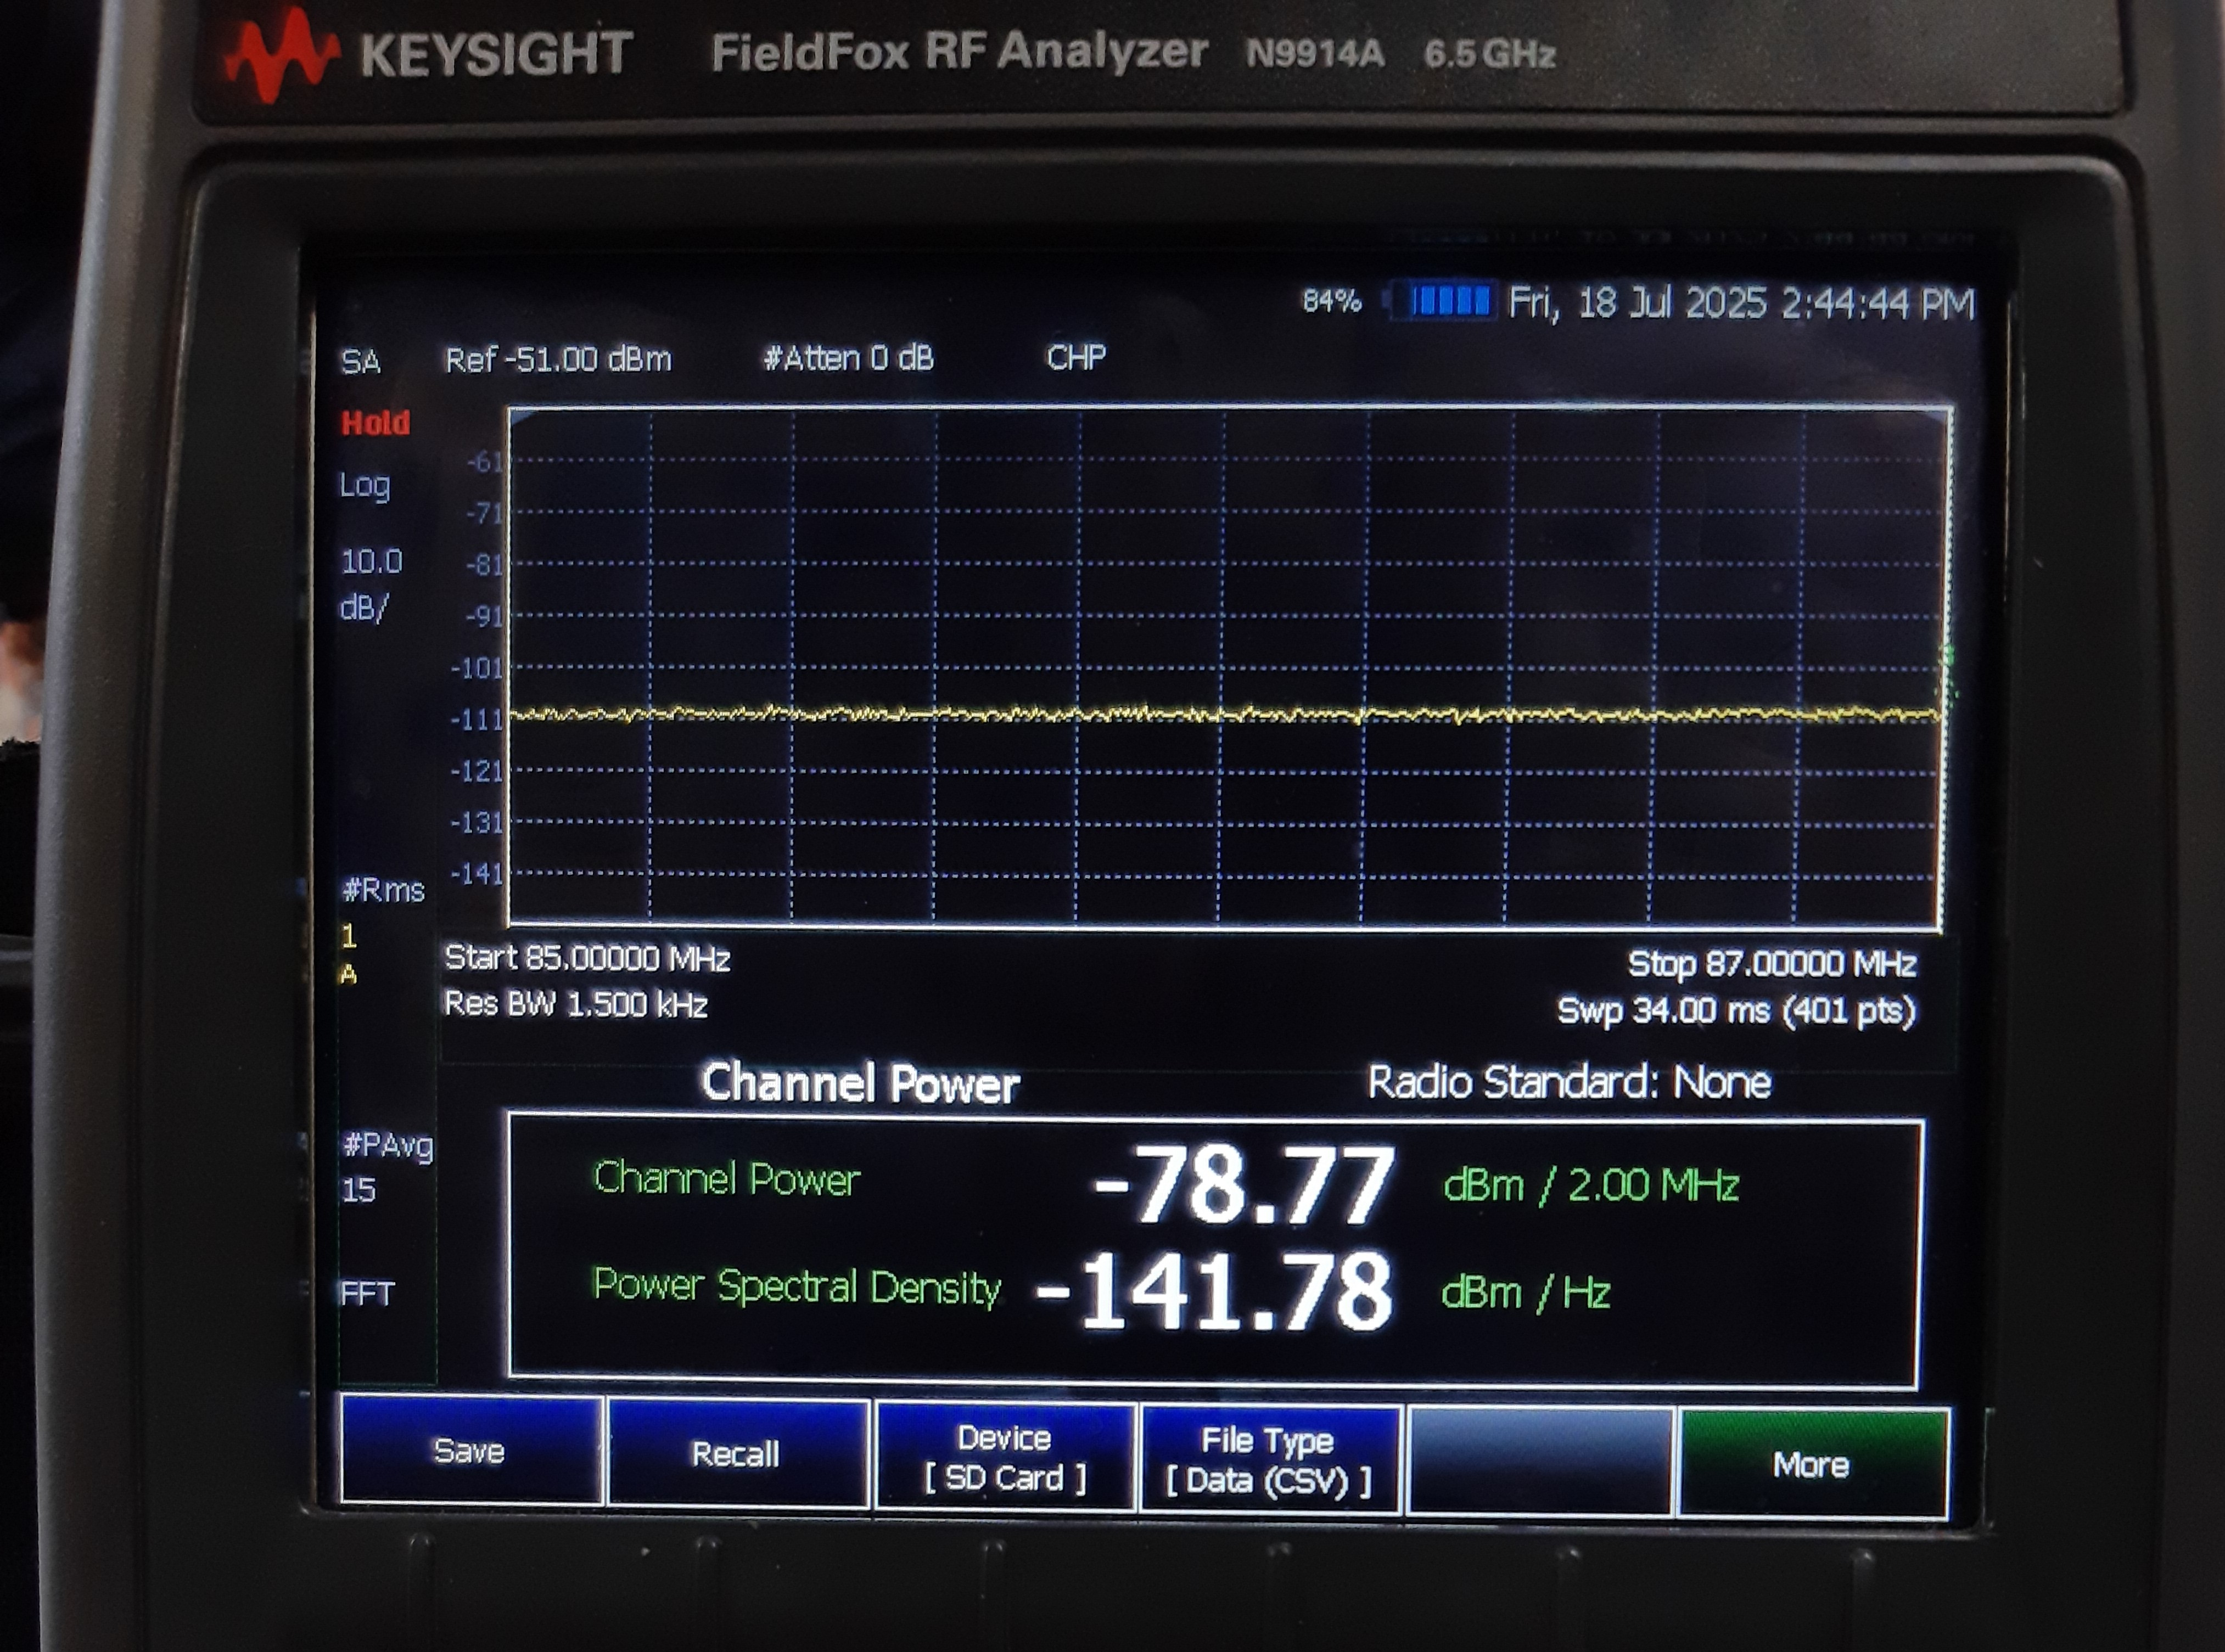
\includegraphics[width=0.4\textwidth]{media/M-Ruido0.5.jpg}
		\caption{Medición de potencia con generador de ruido a 0.3 m}
		\label{fig:M-Ruido0.5}
	\end{figure}
	
	\begin{figure}[h]
		\centering
		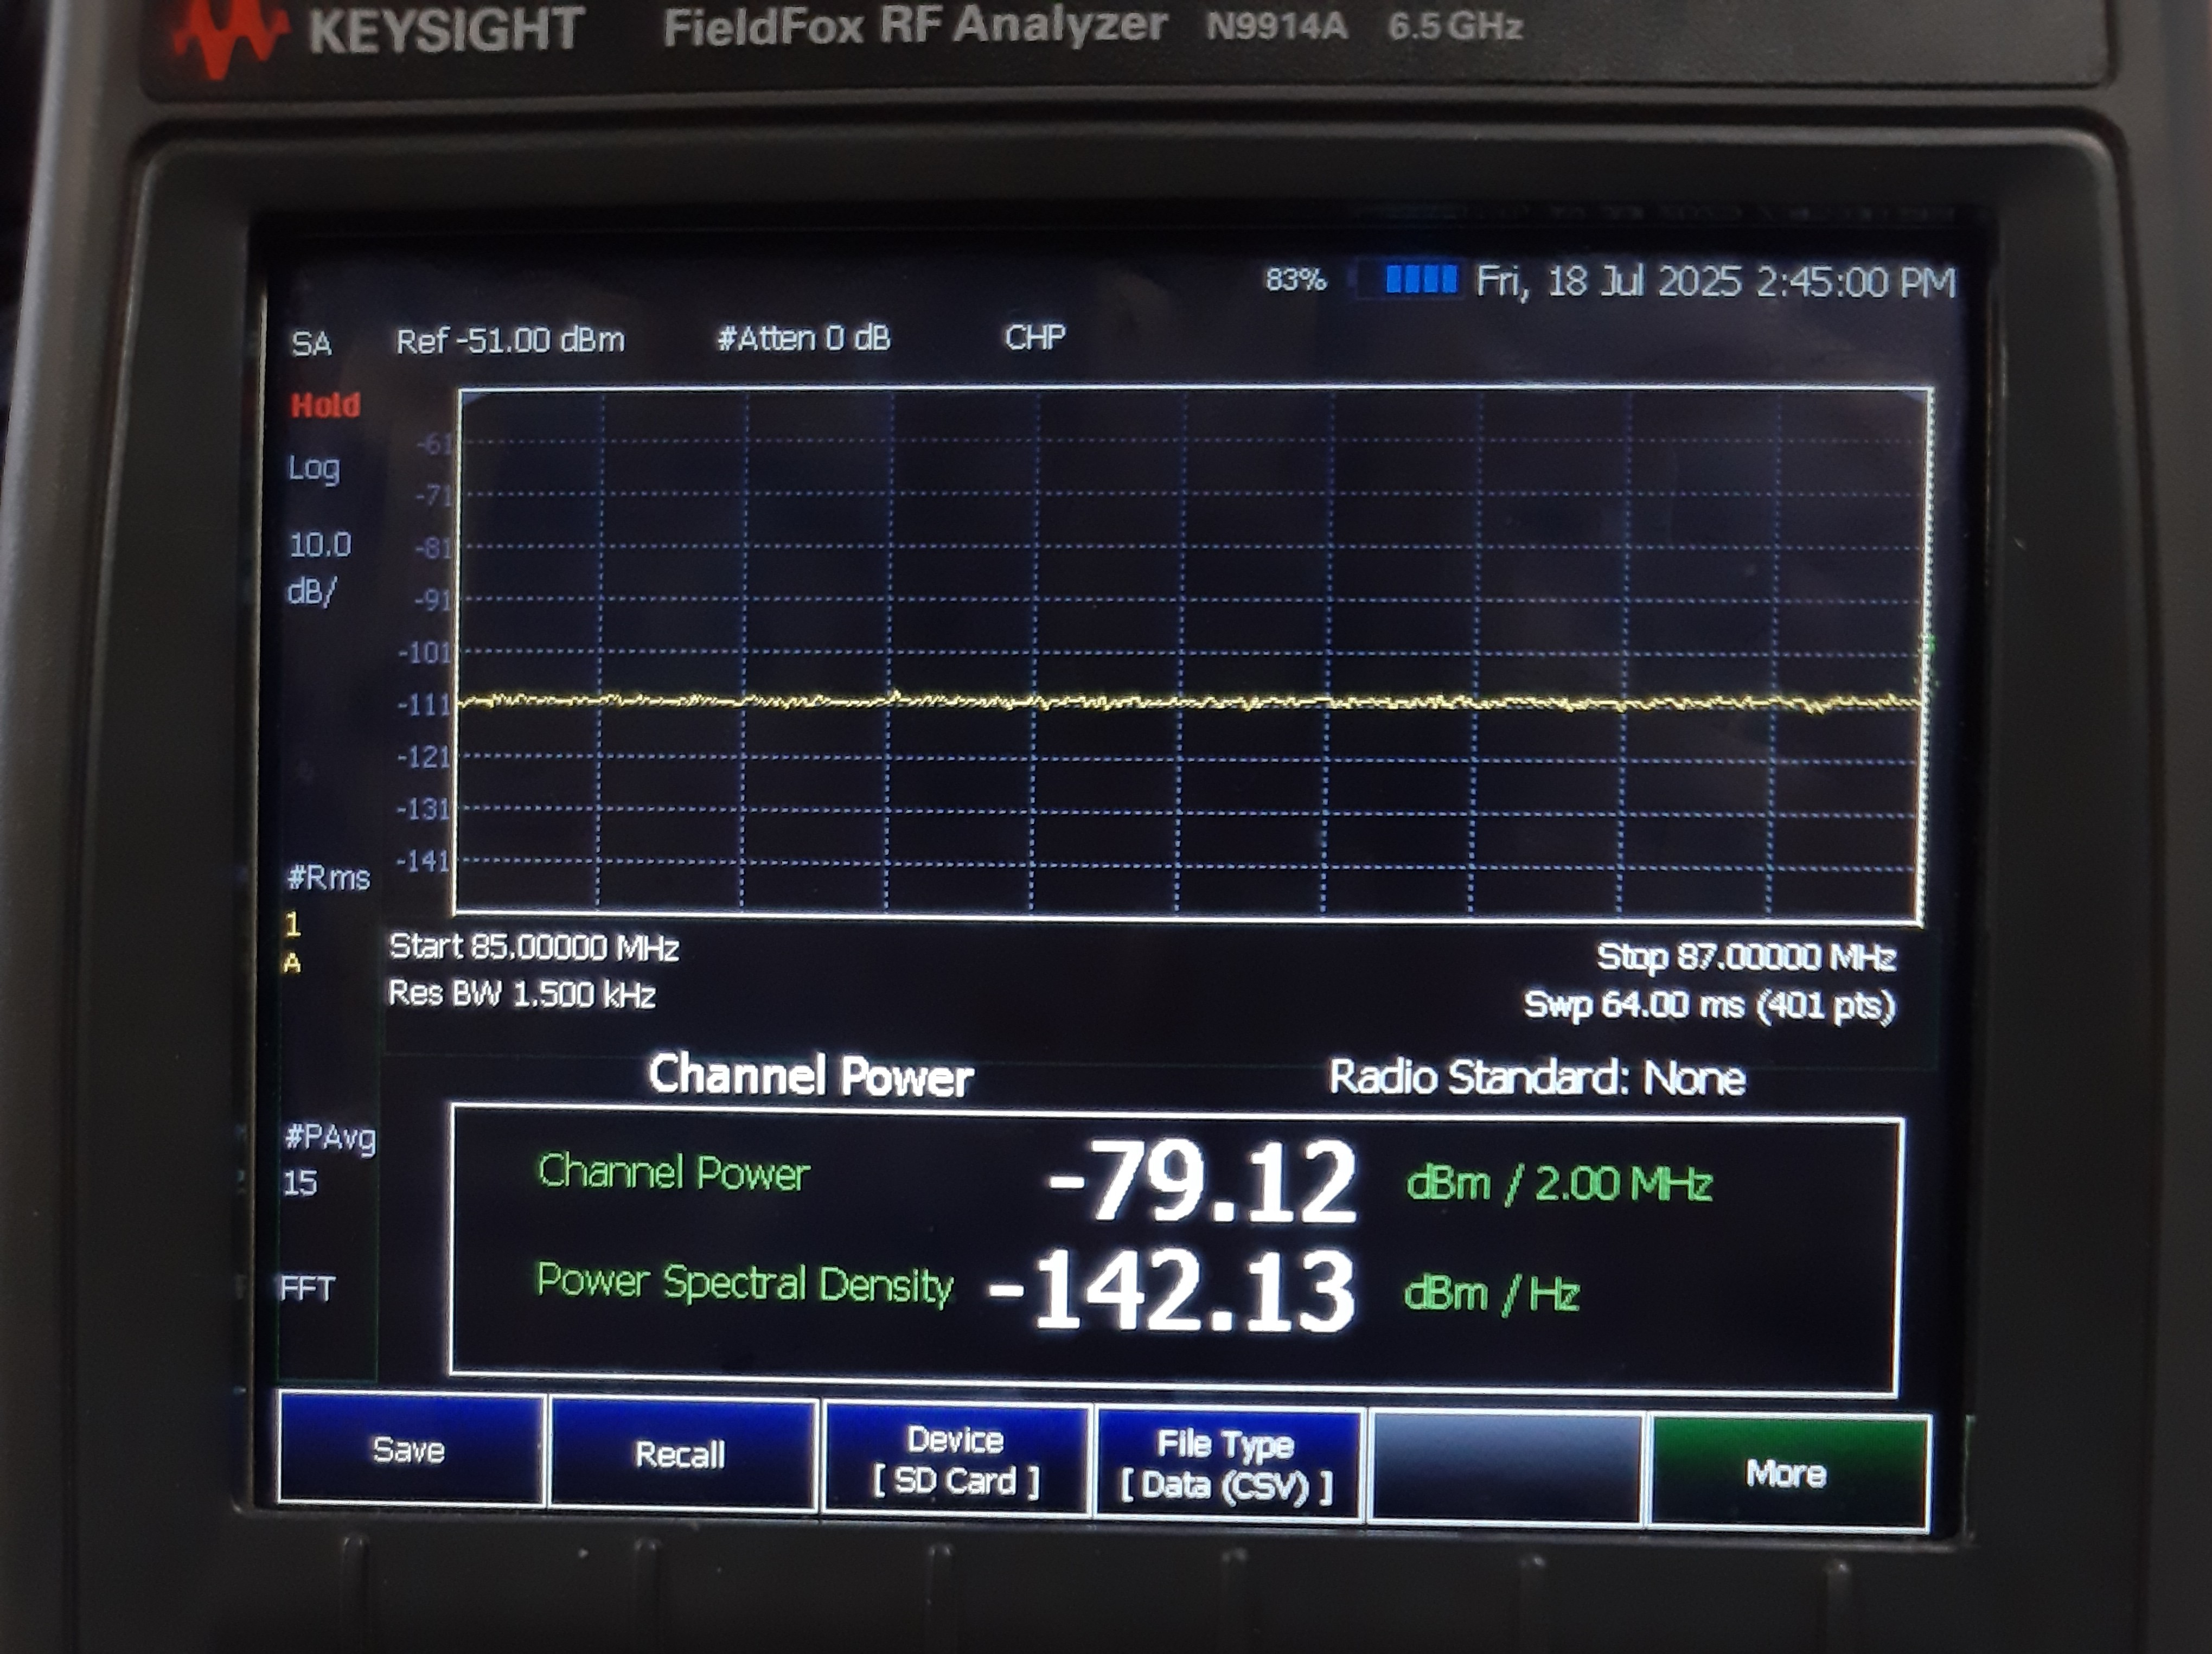
\includegraphics[width=0.4\textwidth]{media/M-Ruido0.3.jpg}
		\caption{Medición de potencia con generador de ruido a 0.3 m}
		\label{fig:M-Ruido0.3}
	\end{figure}
	
	\newpage
	
	\subsection{Anexo B: Mediciones transmitiendo con un $\beta =5$ y añadiendo ruido}
	
	\begin{figure}[h]
		\centering
		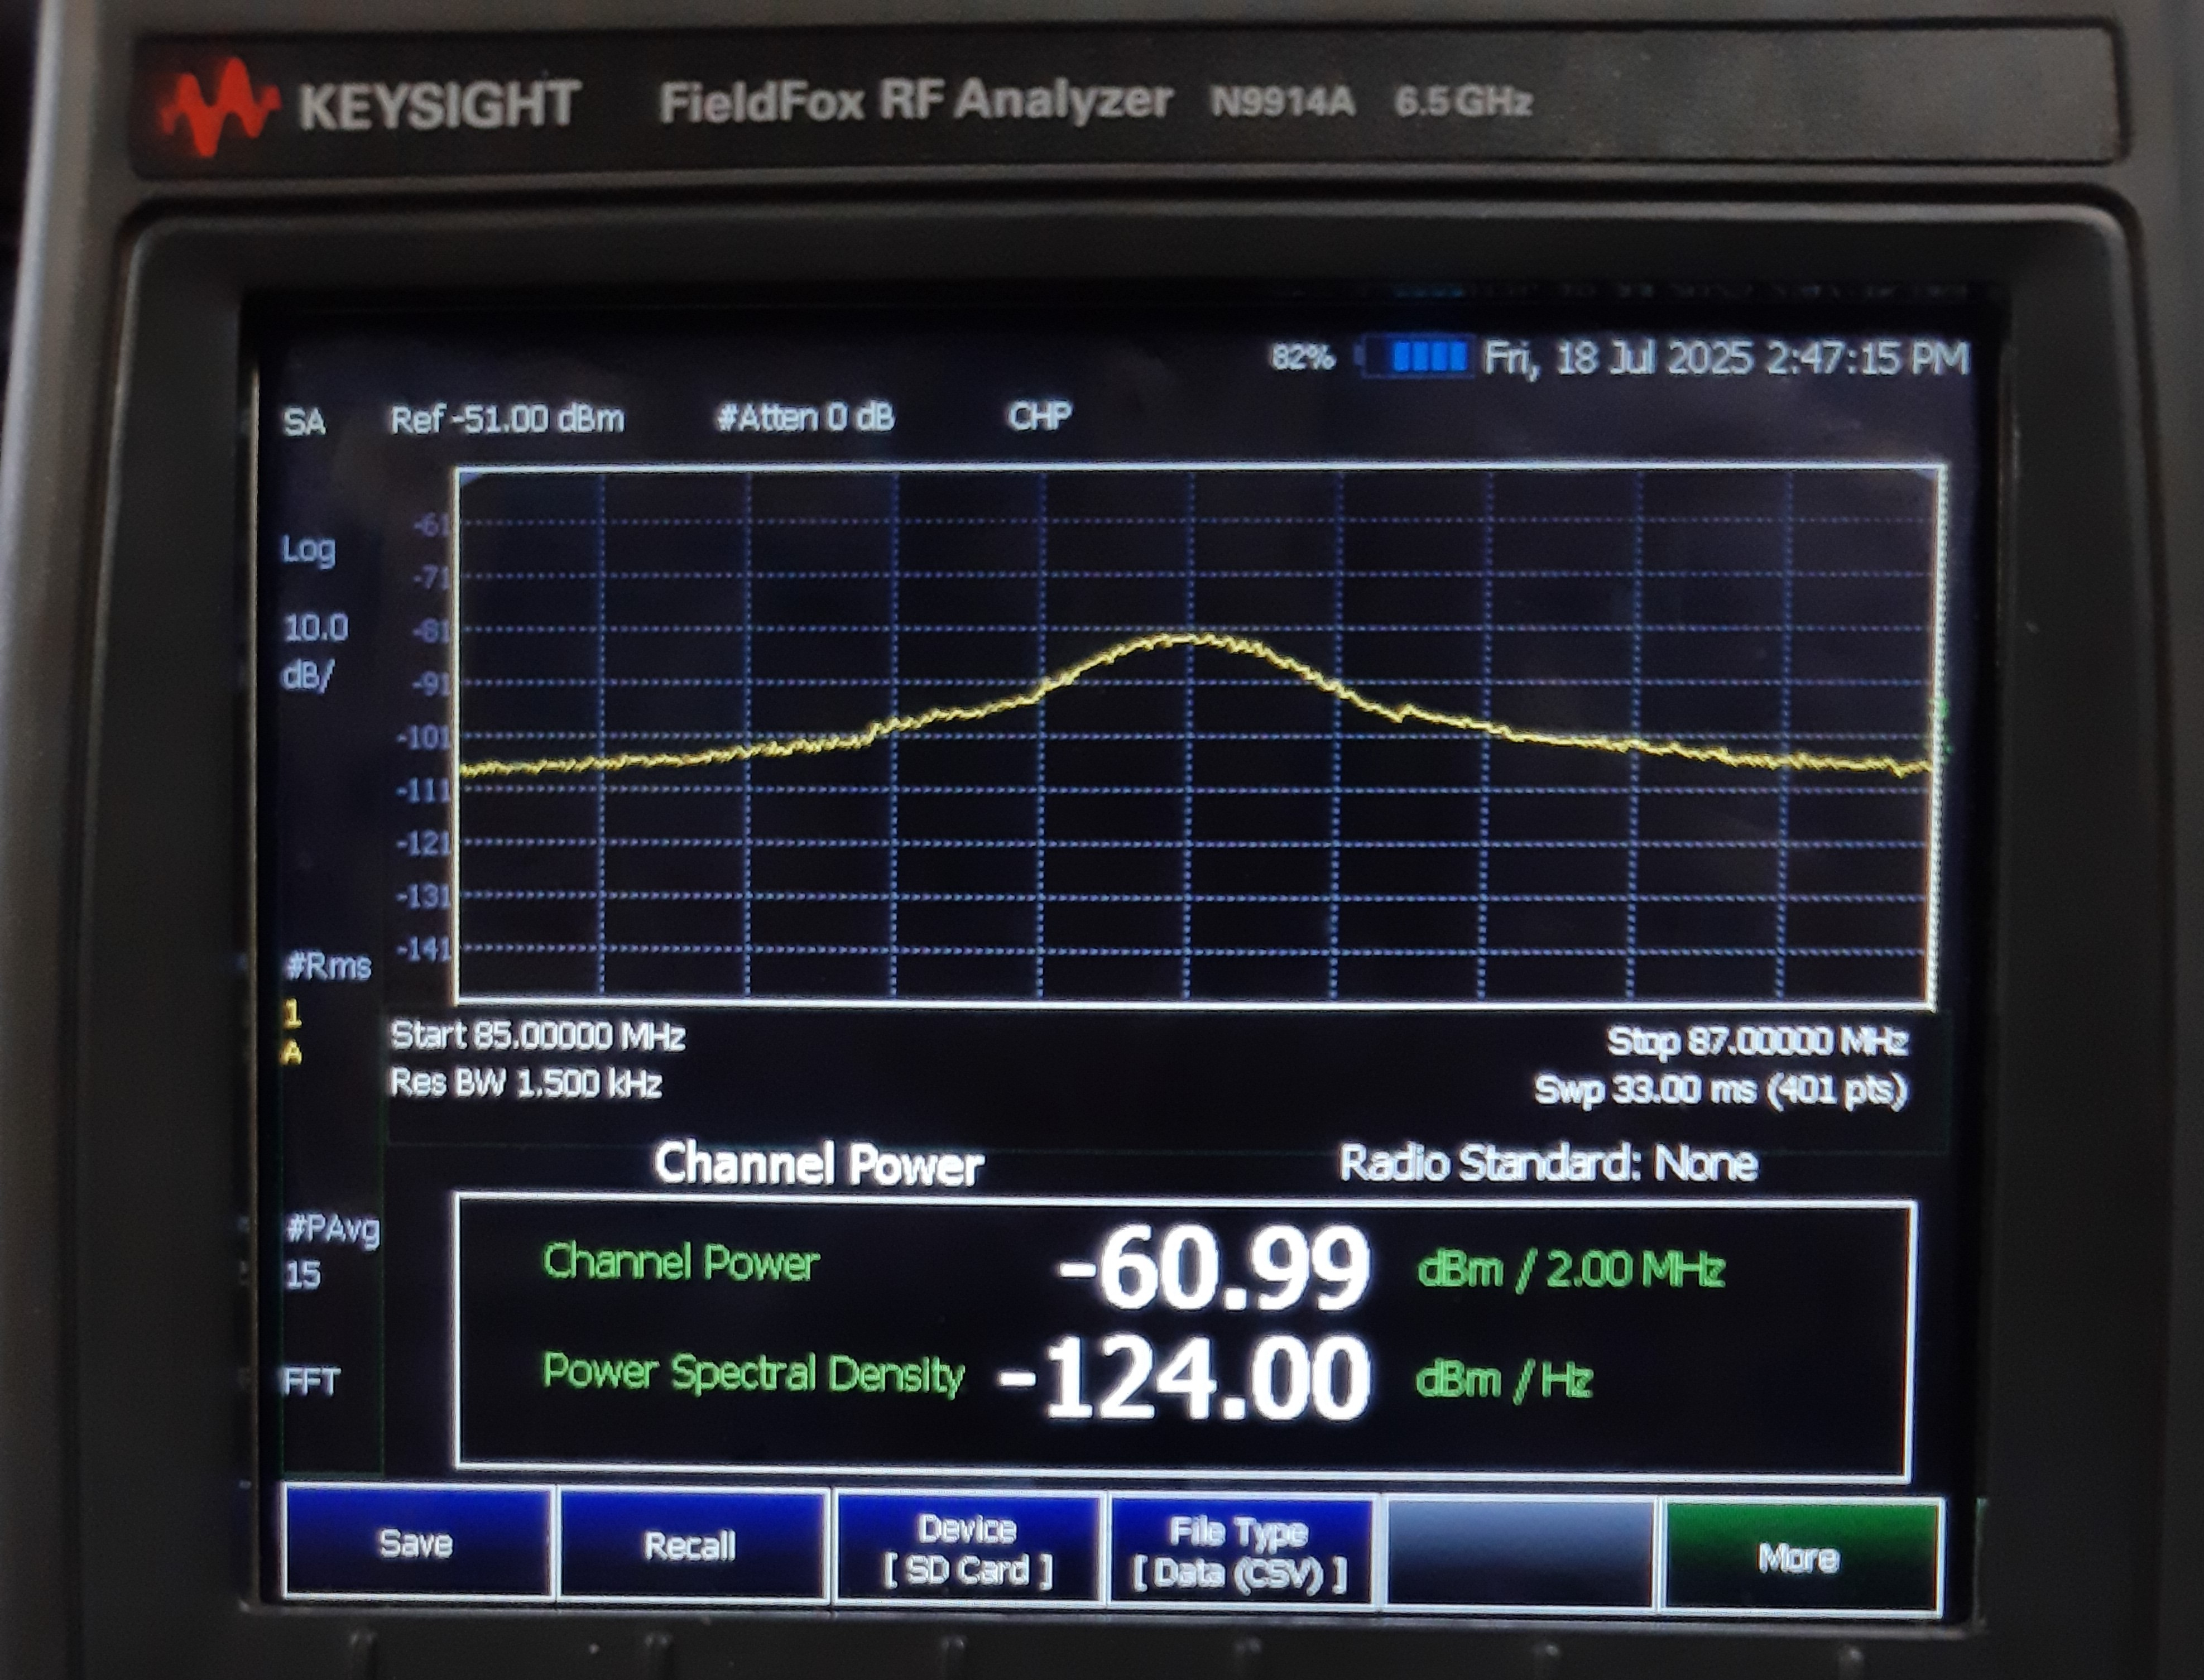
\includegraphics[width=0.4\textwidth]{media/M-S5+R2.jpg}
		\caption{Medición de potencia transmitiendo y con el generador de ruido a 2 m}
		\label{fig:M-S5+R2}
	\end{figure}
	
	\begin{figure}[h]
		\centering
		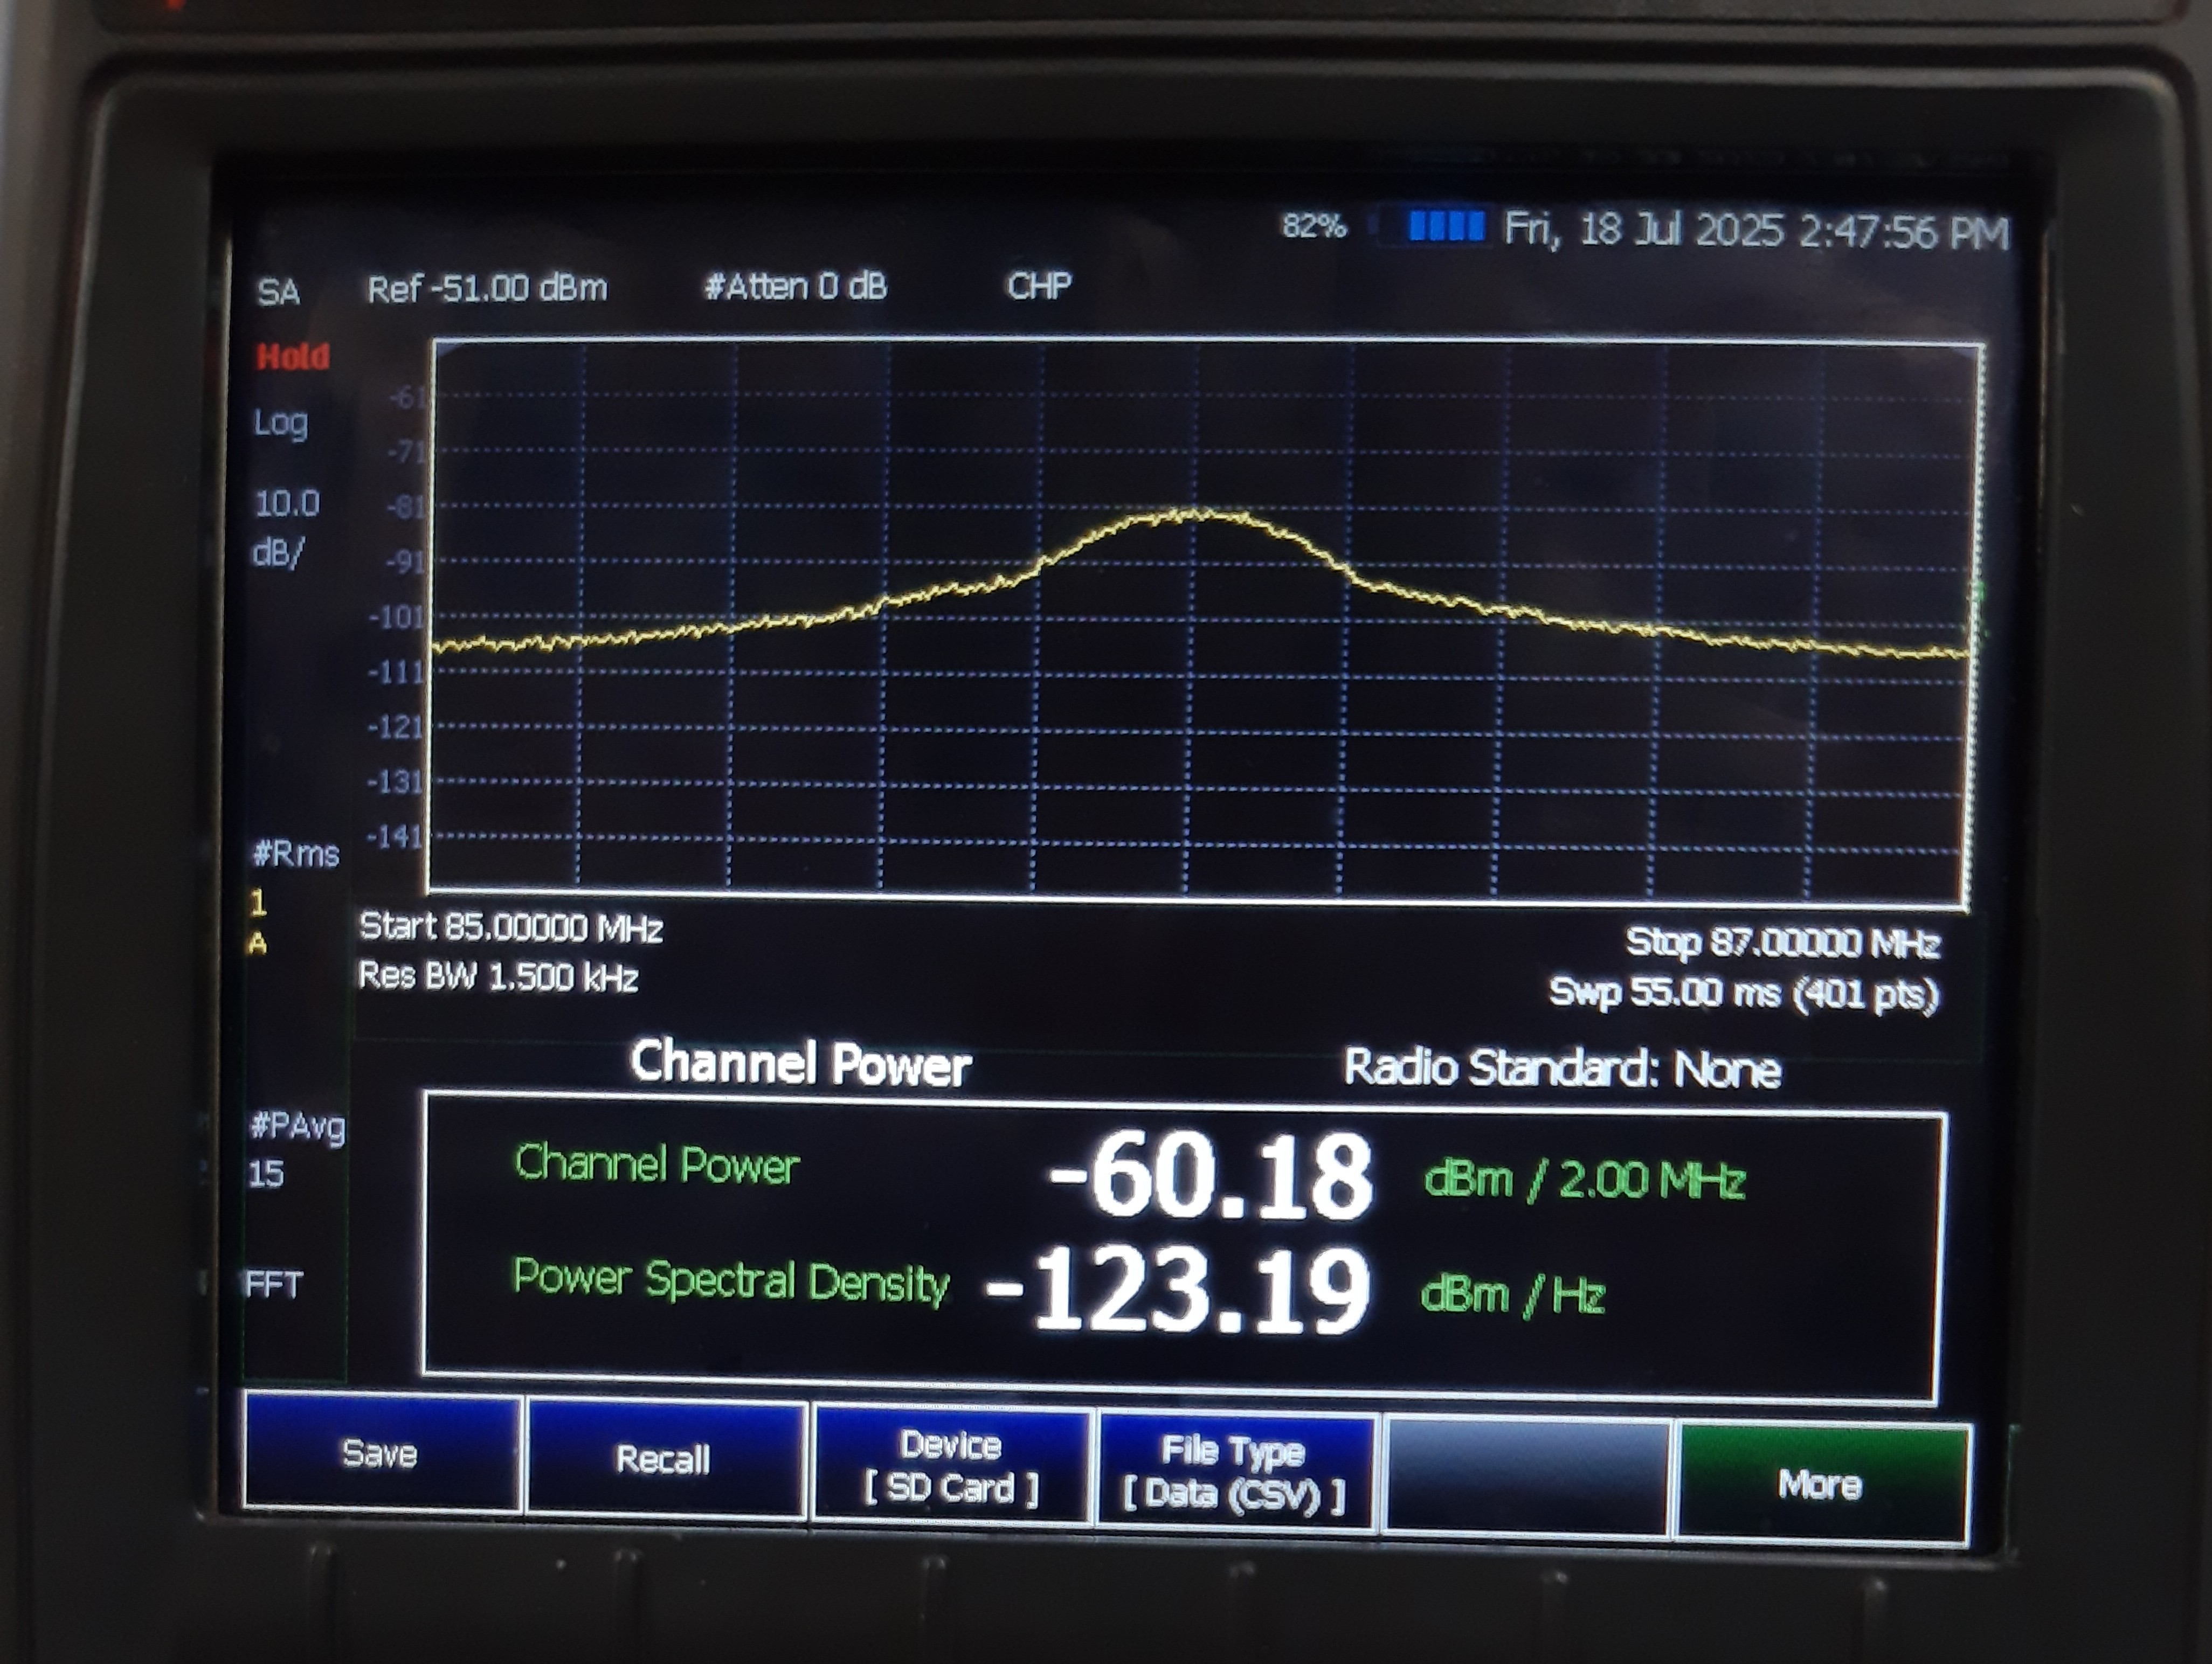
\includegraphics[width=0.4\textwidth]{media/M-S5+R1.jpg}
		\caption{Medición de potencia transmitiendo y con el generador de ruido a 1 m}
		\label{fig:M-S5+R1}
	\end{figure}
	
	\begin{figure}[h]
		\centering
		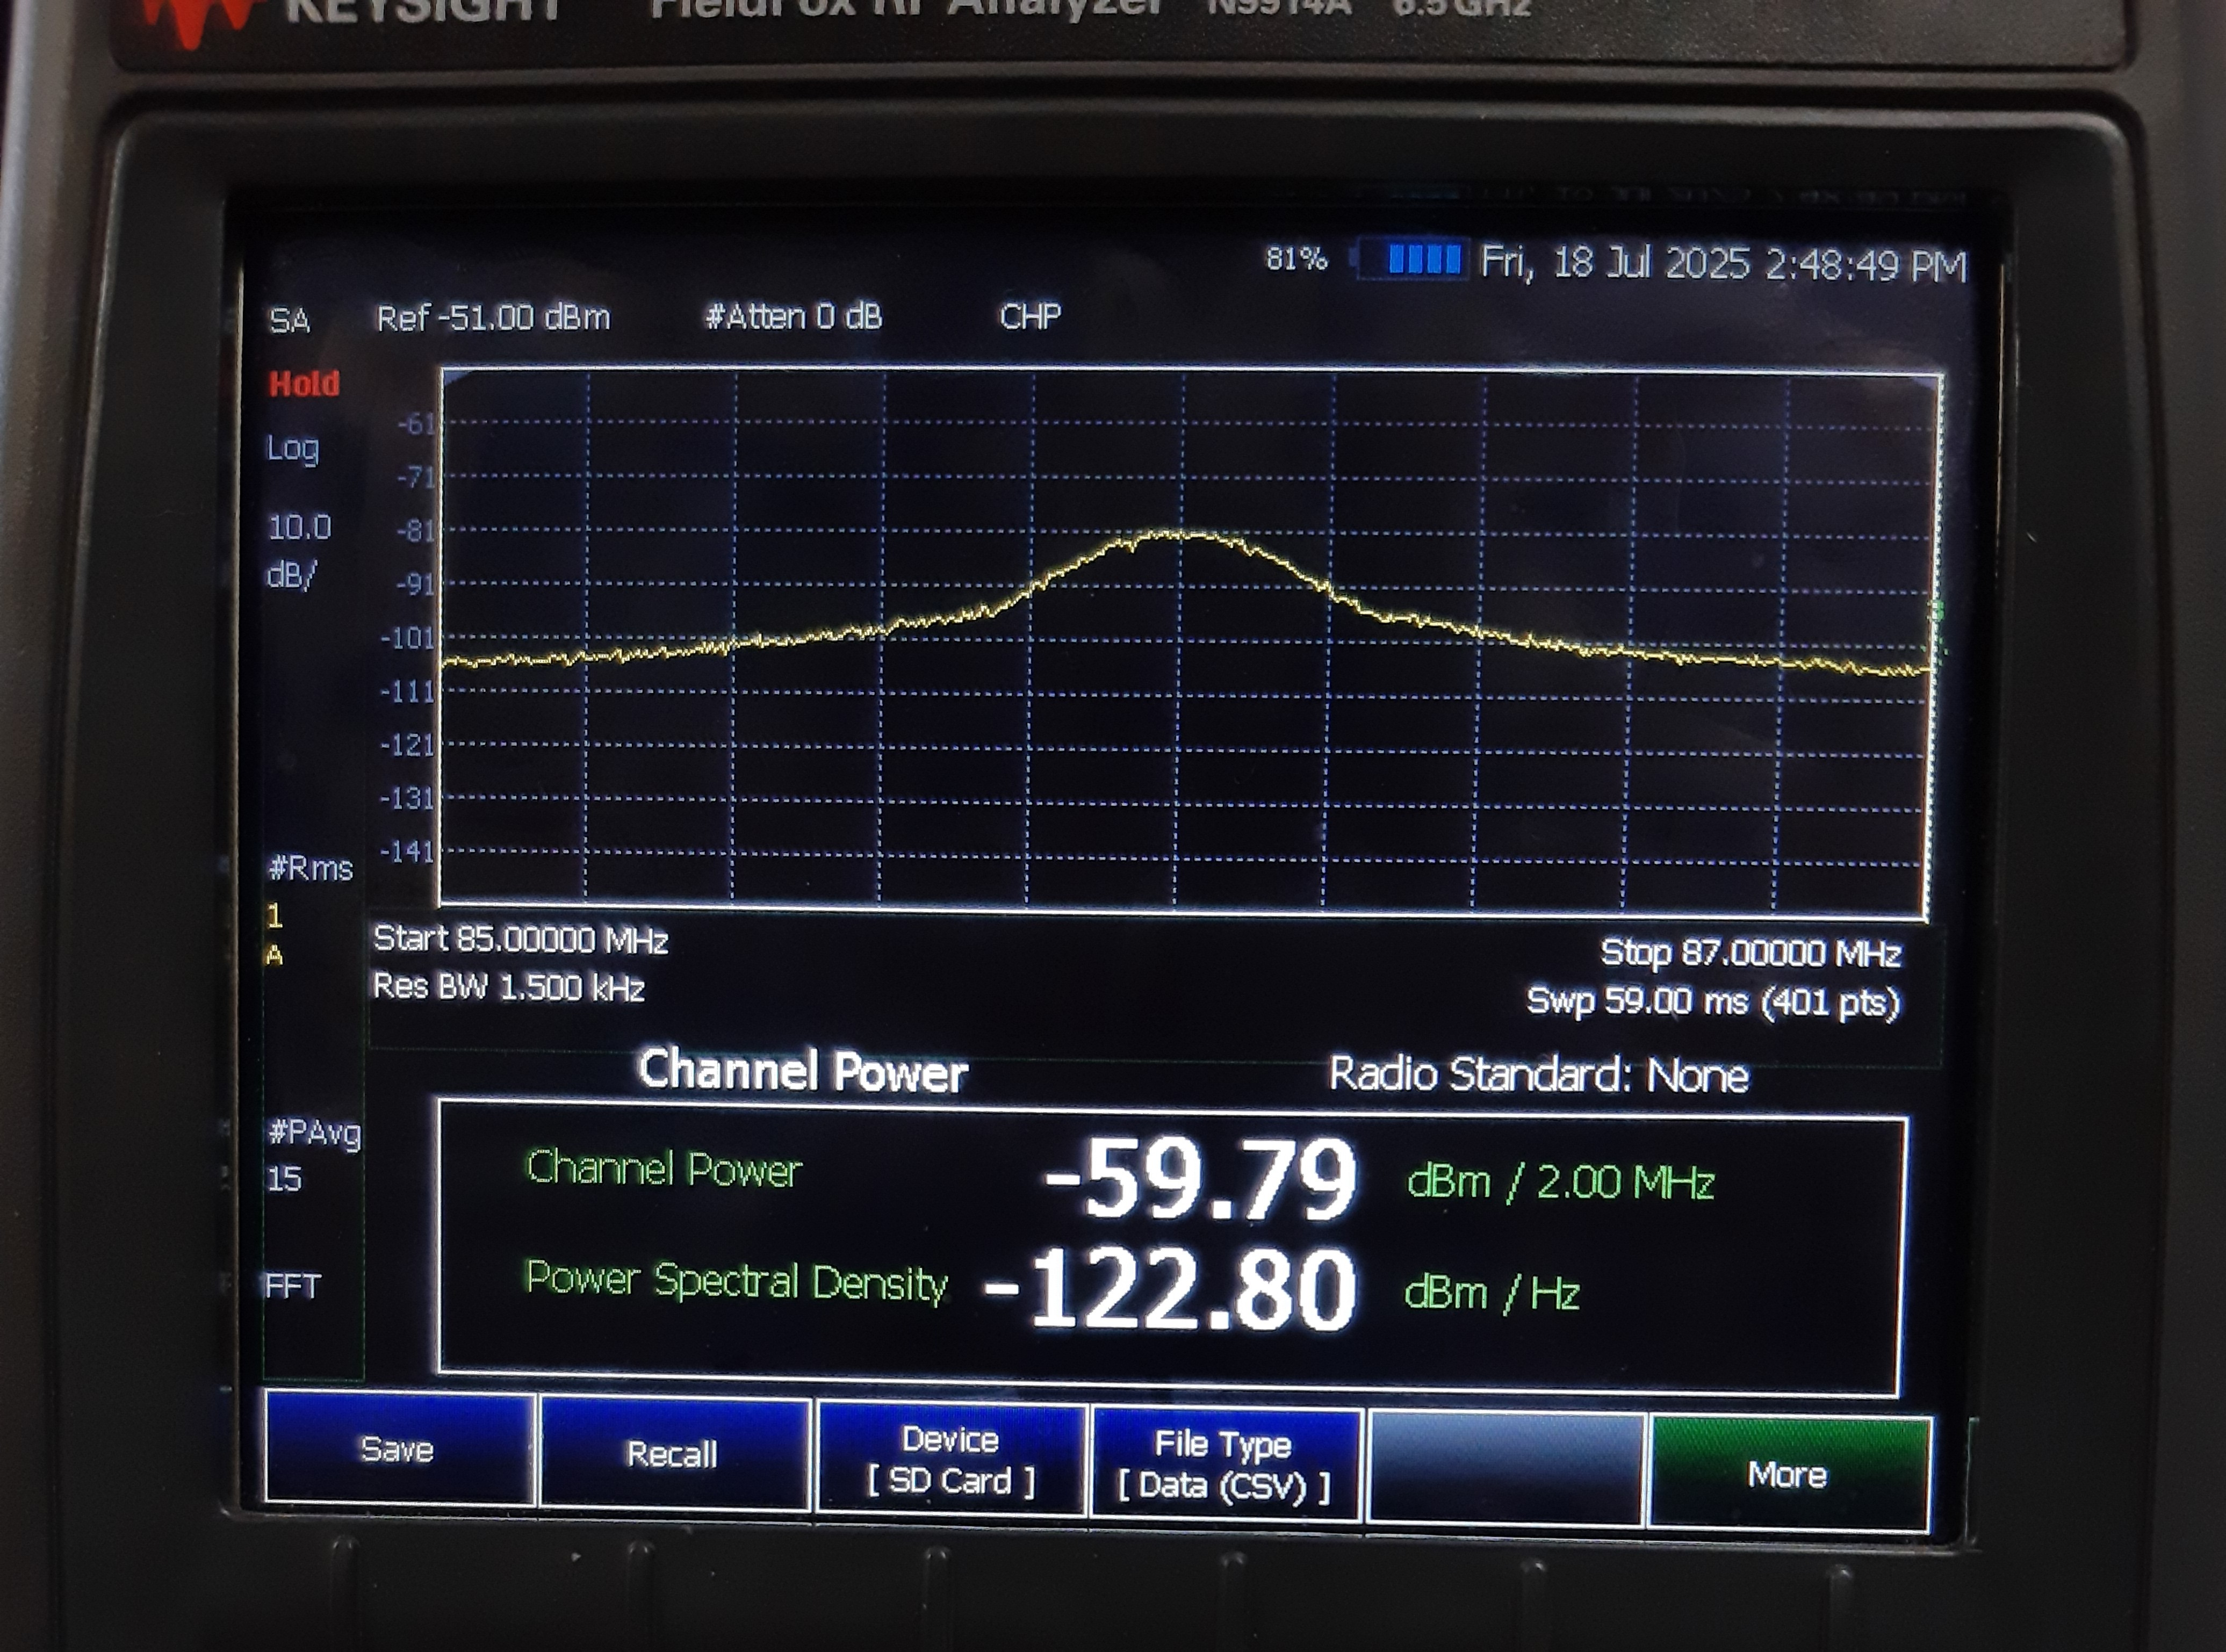
\includegraphics[width=0.4\textwidth]{media/M-S5+R0.5.jpg}
		\caption{Medición de potencia transmitiendo y con el generador de ruido a 0.5 m}
		\label{fig:M-S5+R.5}
	\end{figure}
	
	\begin{figure}[h]
		\centering
		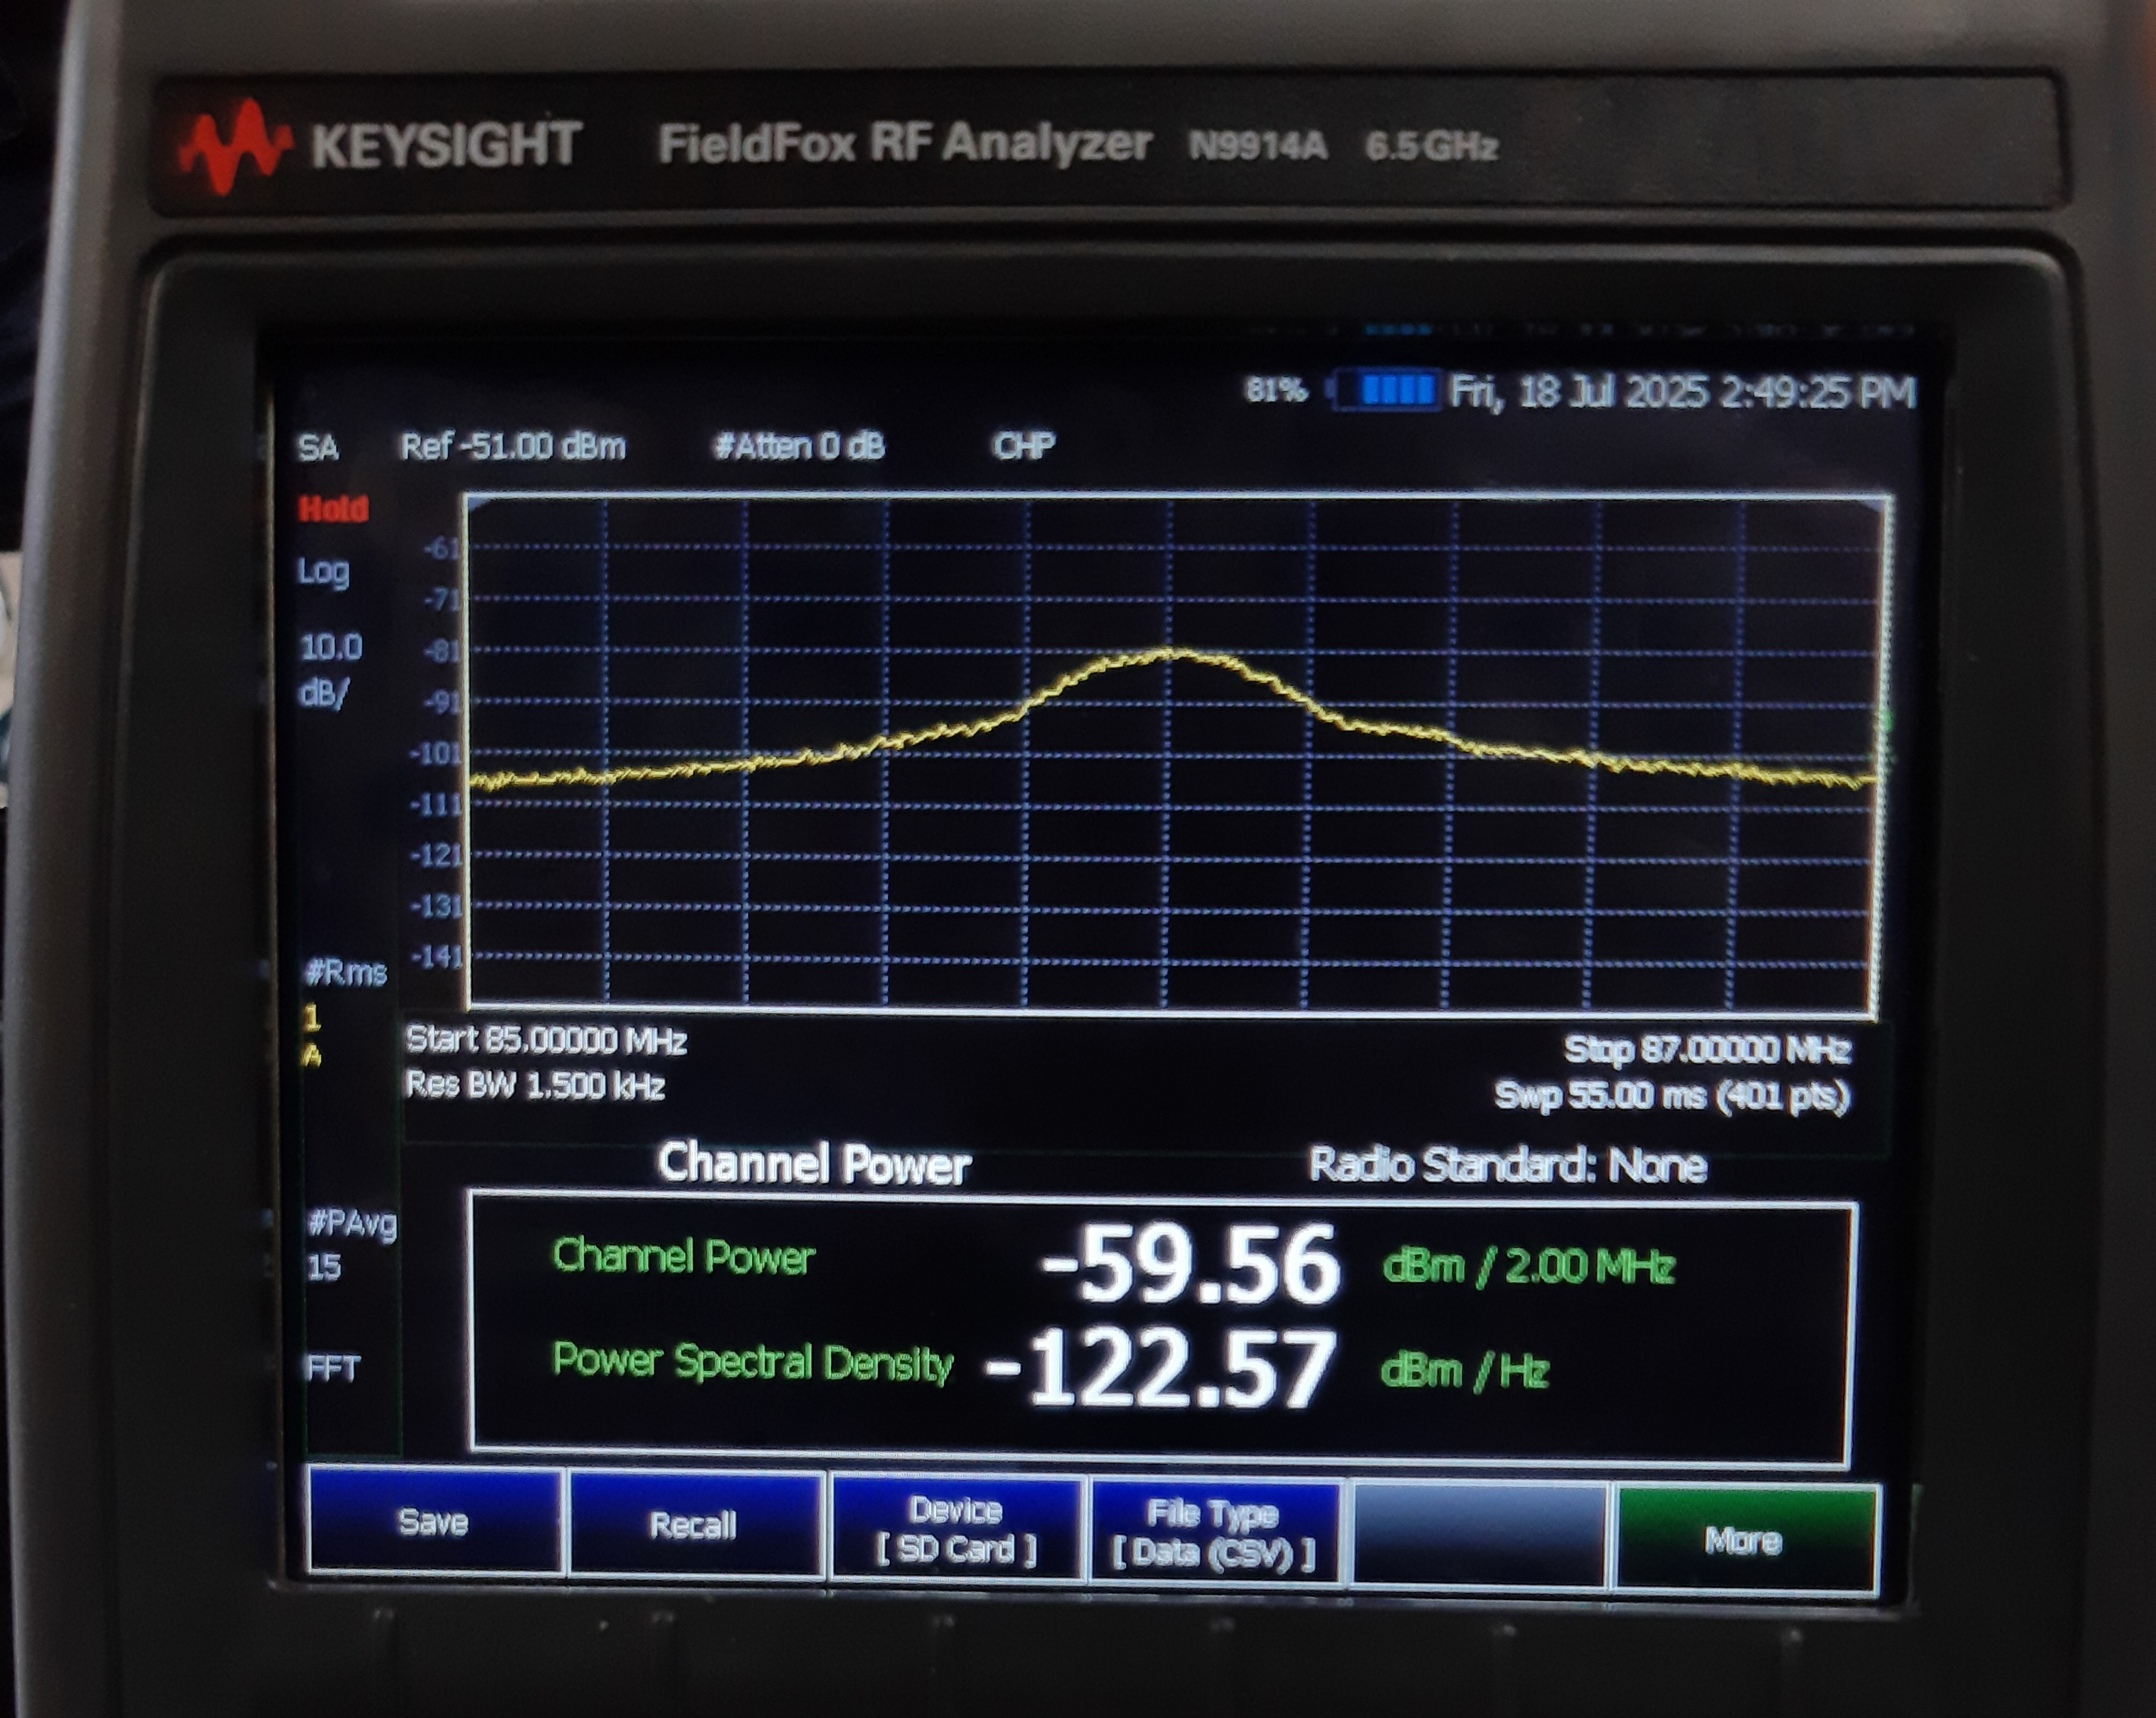
\includegraphics[width=0.4\textwidth]{media/M-S5+R0.3.jpg}
		\caption{Medición de potencia transmitiendo y con el generador de ruido a 0.3 m}
		\label{fig:M-S5+R0.3}
	\end{figure}
	
	
	\subsection{Anexo C: Mediciones transmitiendo con un $\beta =6$ y añadiendo ruido}
	
	\begin{figure}[h]
		\centering
		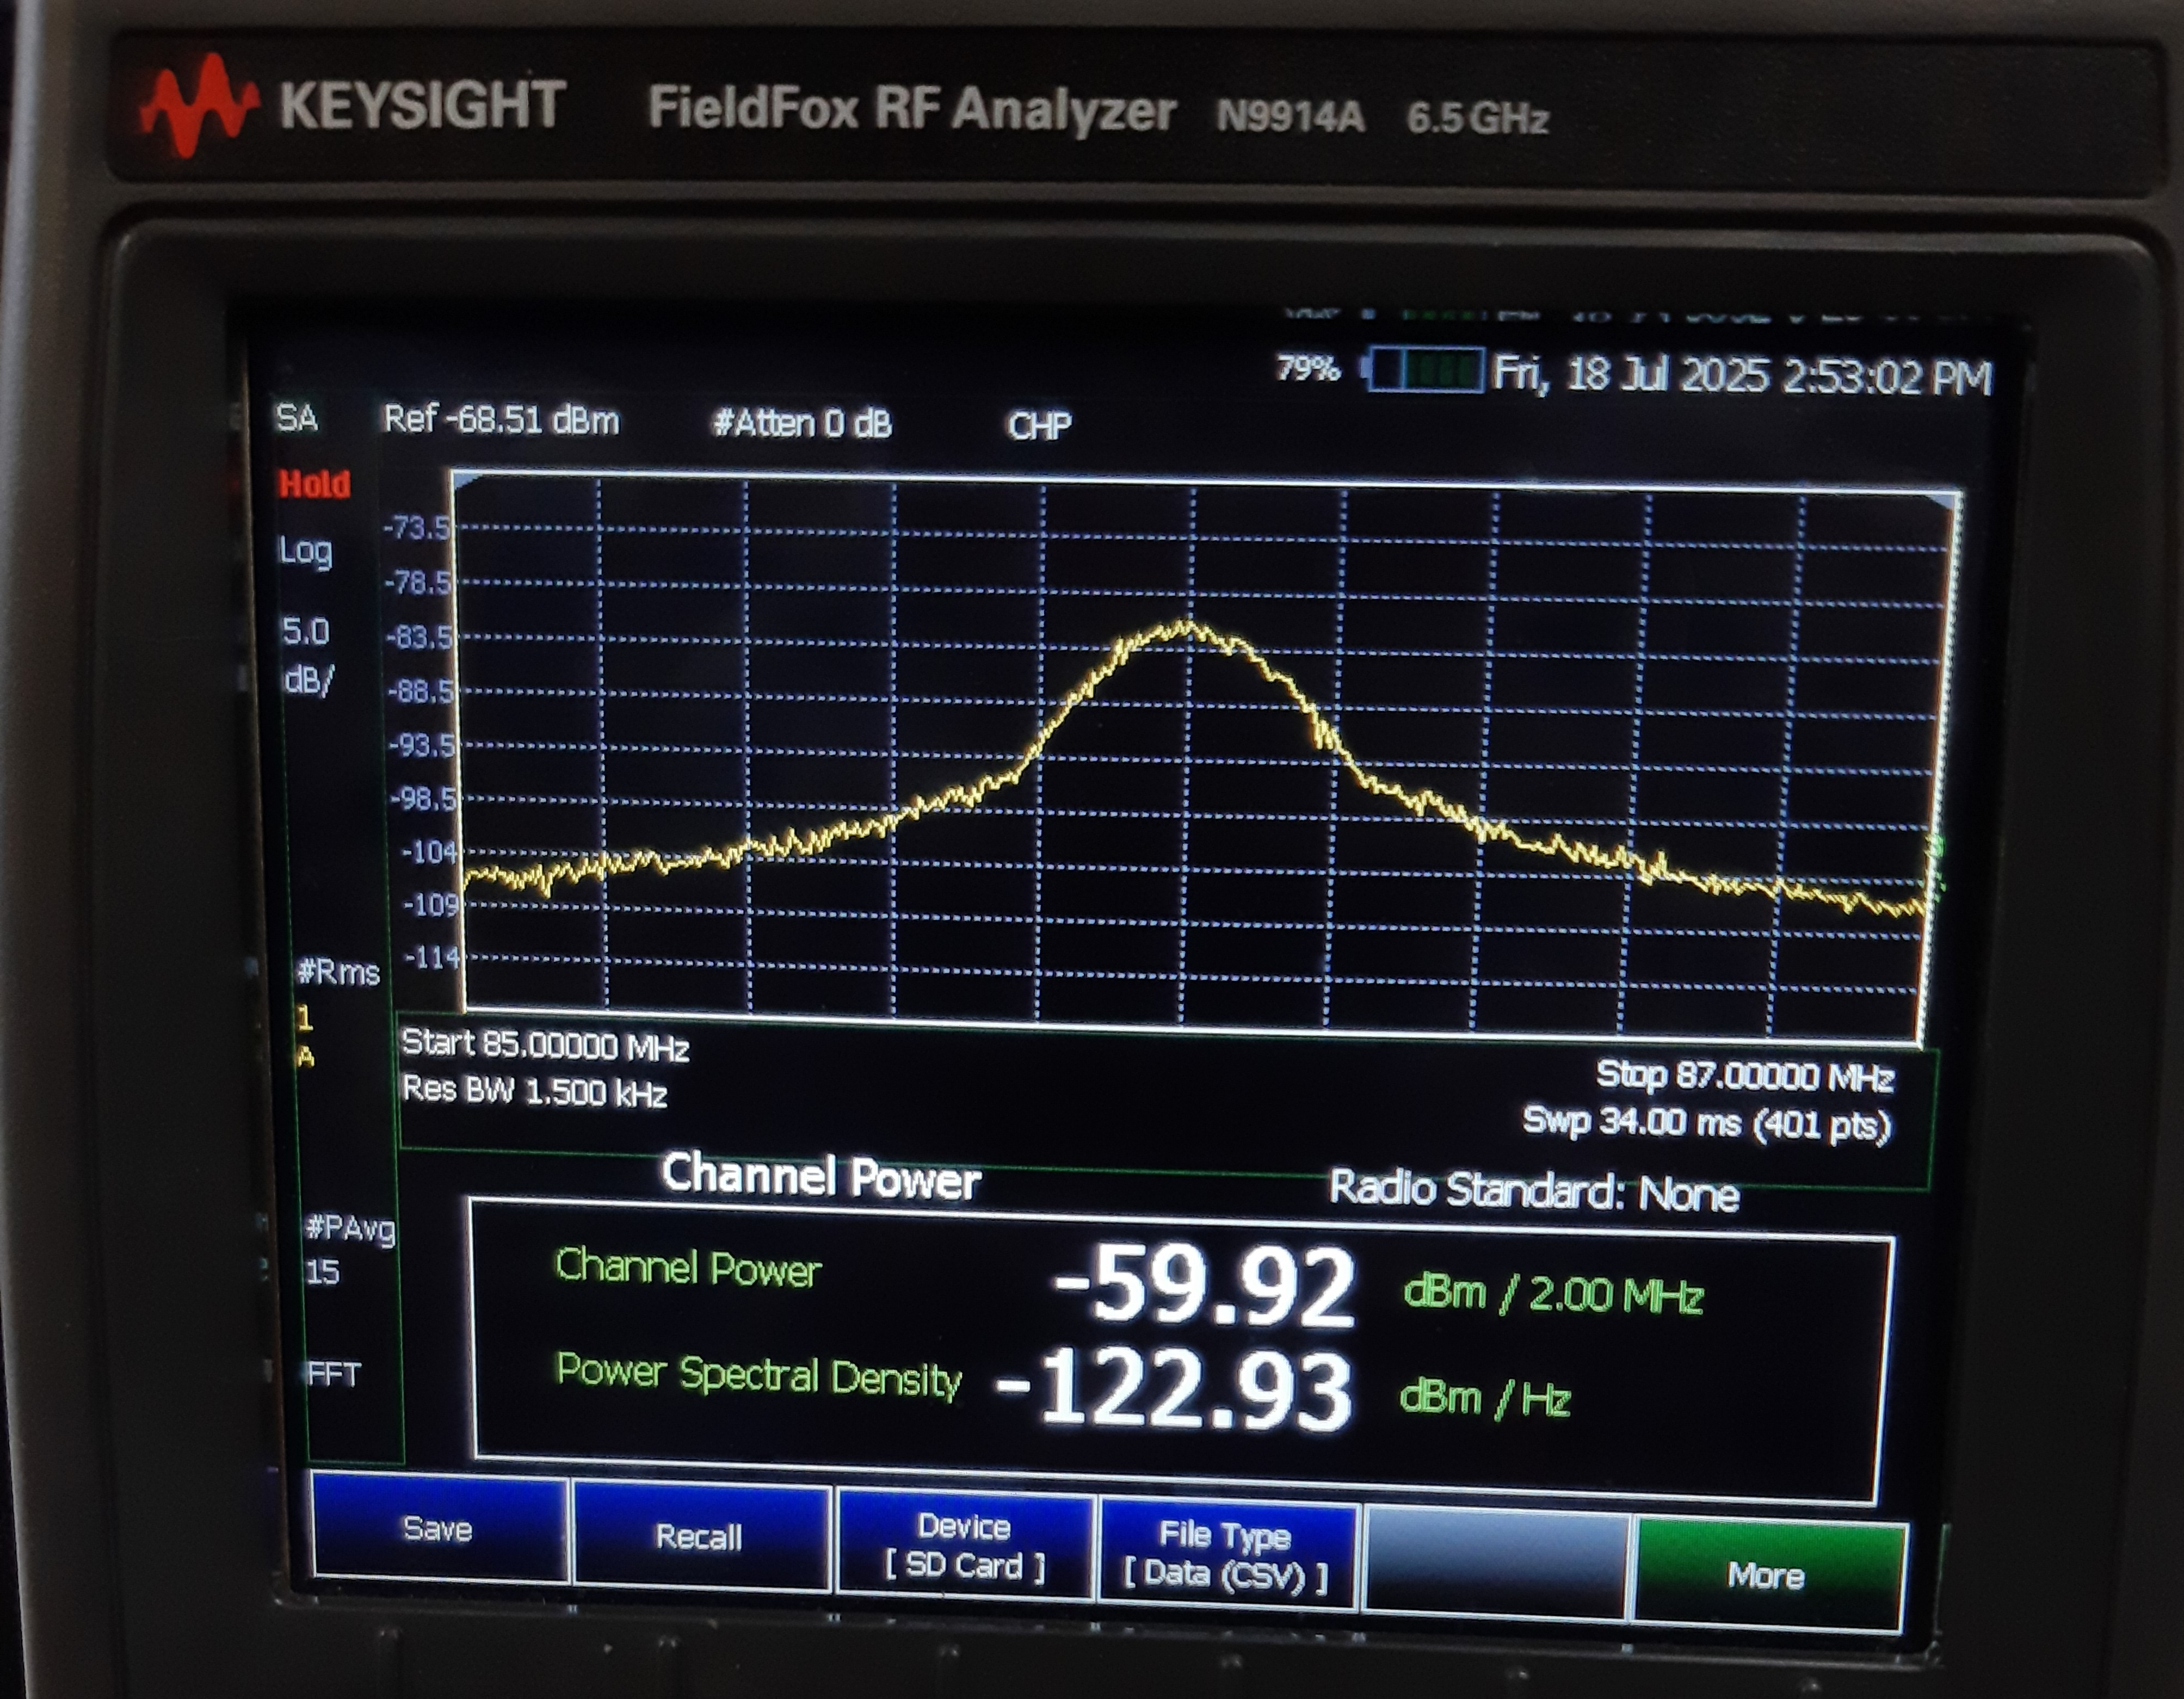
\includegraphics[width=0.4\textwidth]{media/M-S6+R2.jpg}
		\caption{Medición de potencia transmitiendo y con el generador de ruido a 2 m}
		\label{fig:M-S6+R2}
	\end{figure}
	
	\begin{figure}[h]
		\centering
		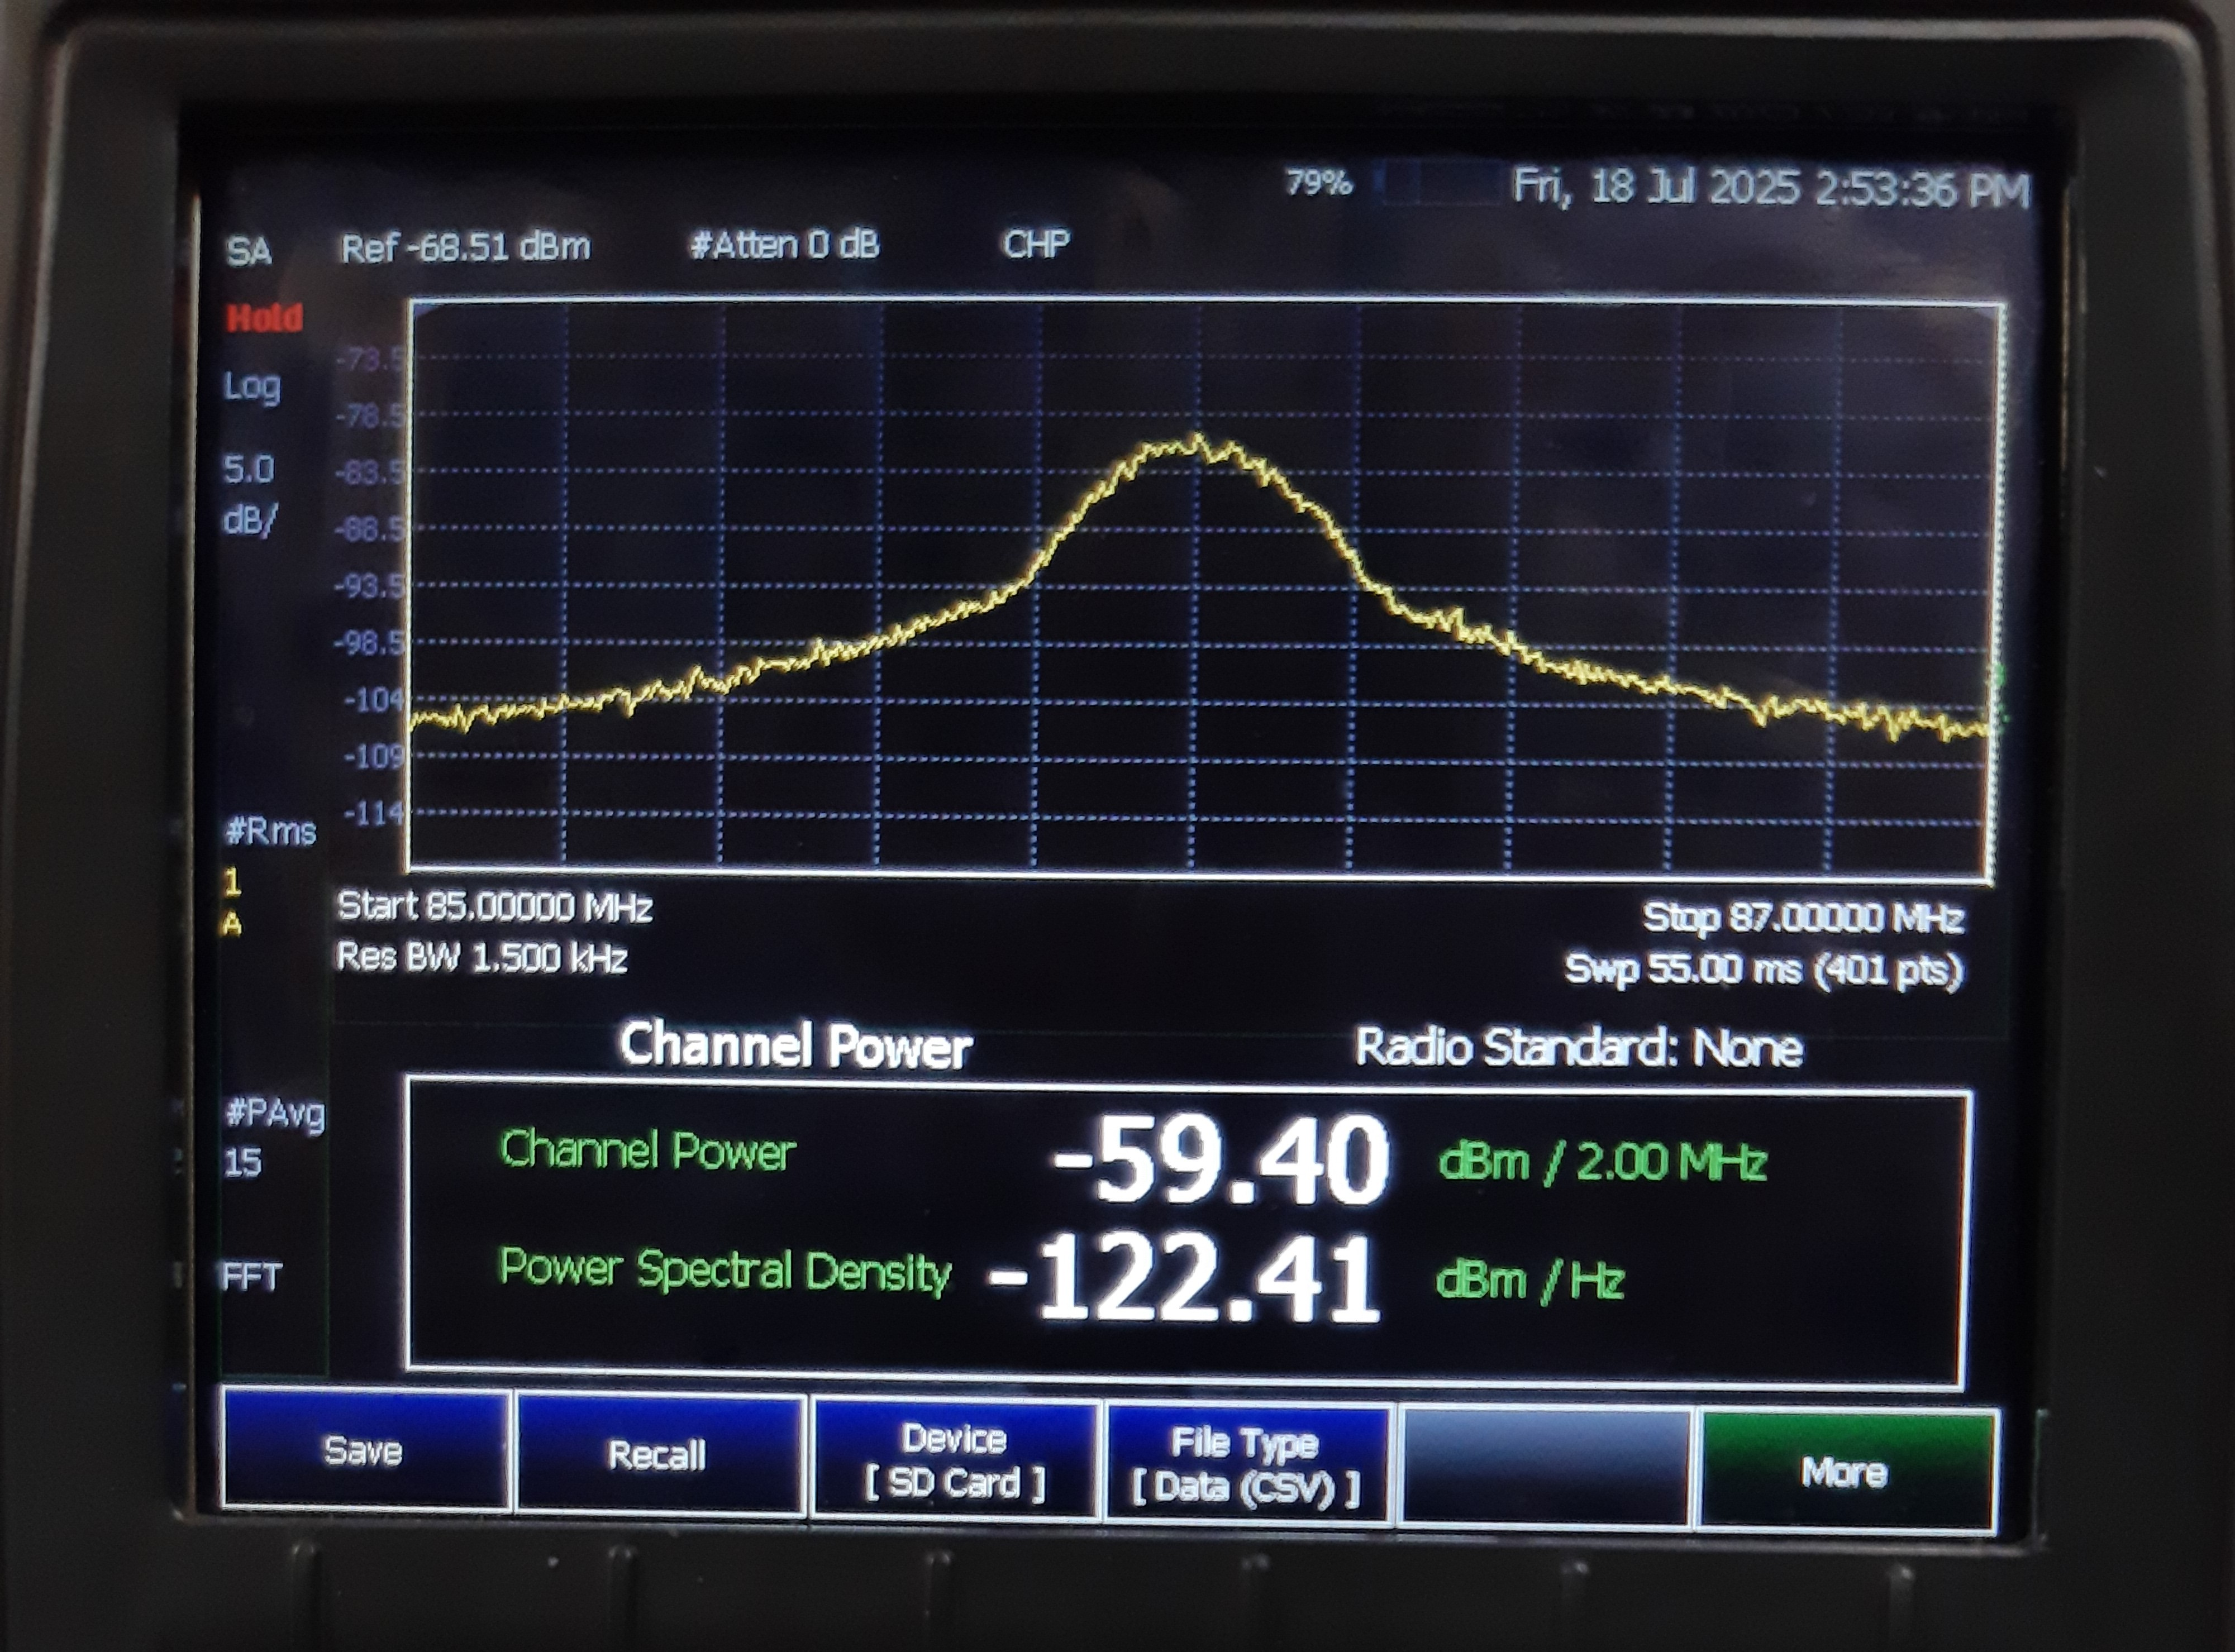
\includegraphics[width=0.4\textwidth]{media/M-S6+R1.jpg}
		\caption{Medición de potencia transmitiendo y con el generador de ruido a 1 m}
		\label{fig:M-S6+R1}
	\end{figure}
	
	\begin{figure}[h]
		\centering
		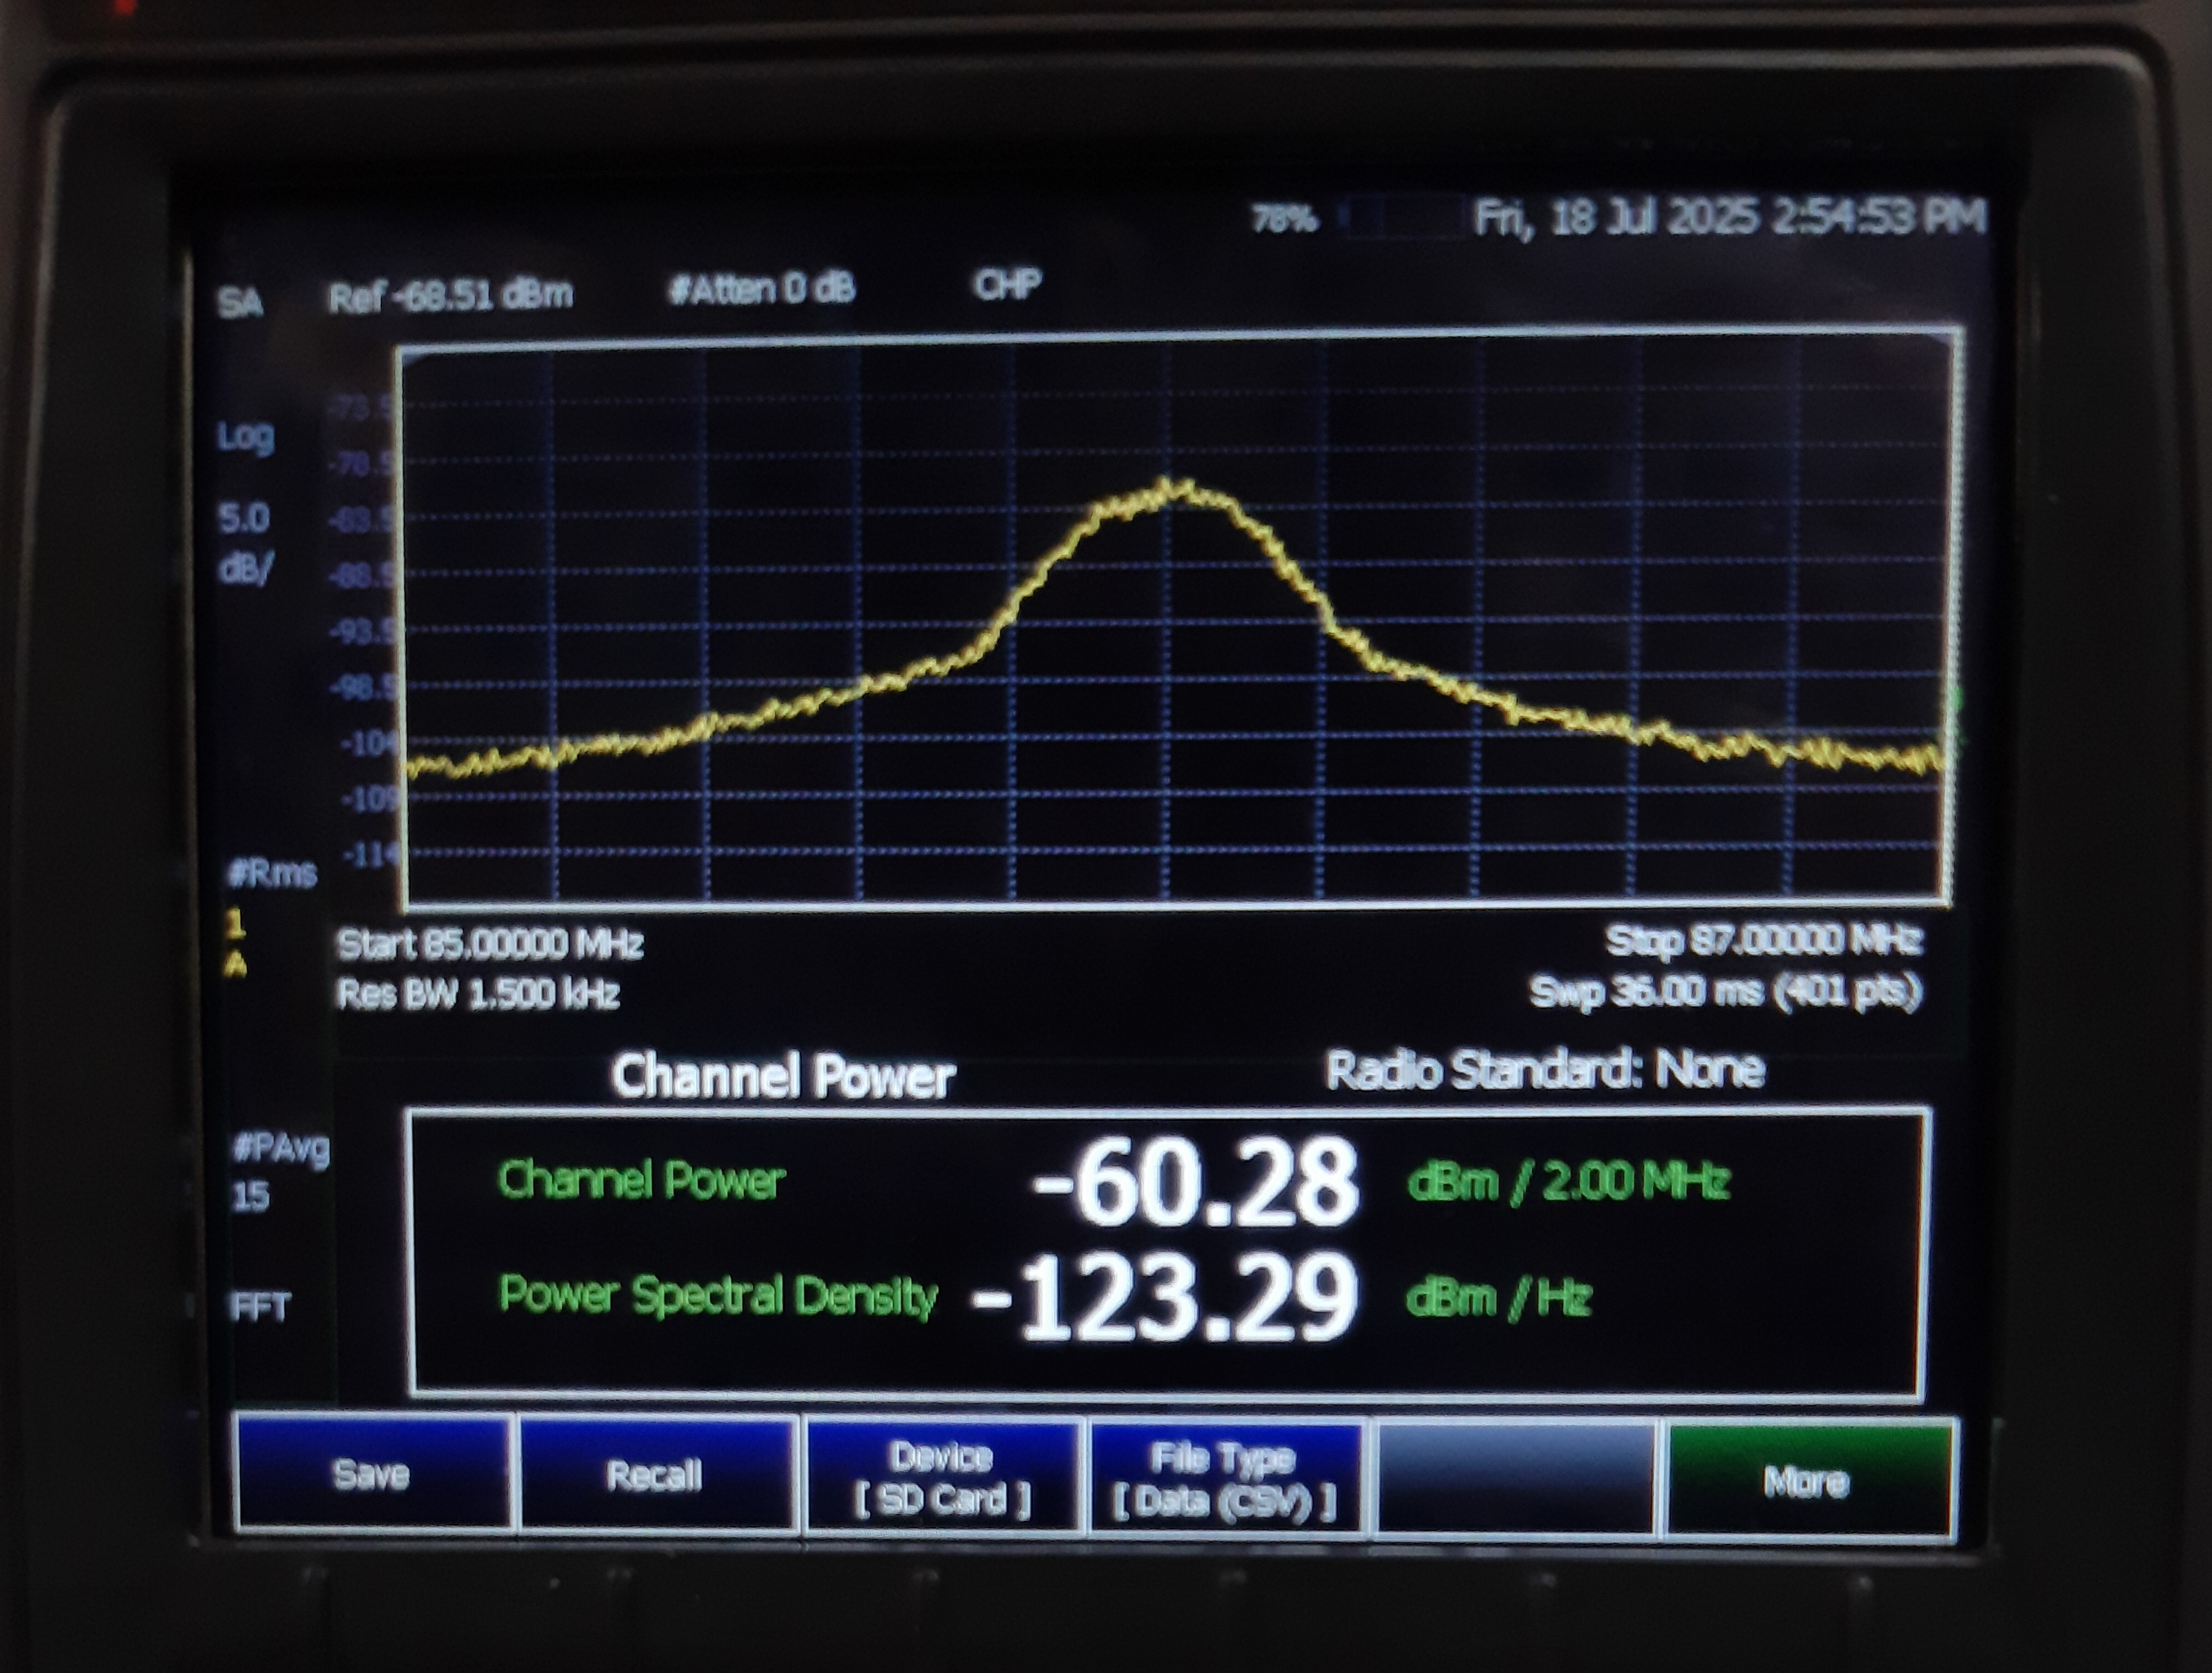
\includegraphics[width=0.4\textwidth]{media/M-S6+R0.5.jpg}
		\caption{Medición de potencia transmitiendo y con el generador de ruido a 0.3 m}
		\label{fig:M-S6+R.5}
	\end{figure}
	
	\begin{figure}[h]
		\centering
		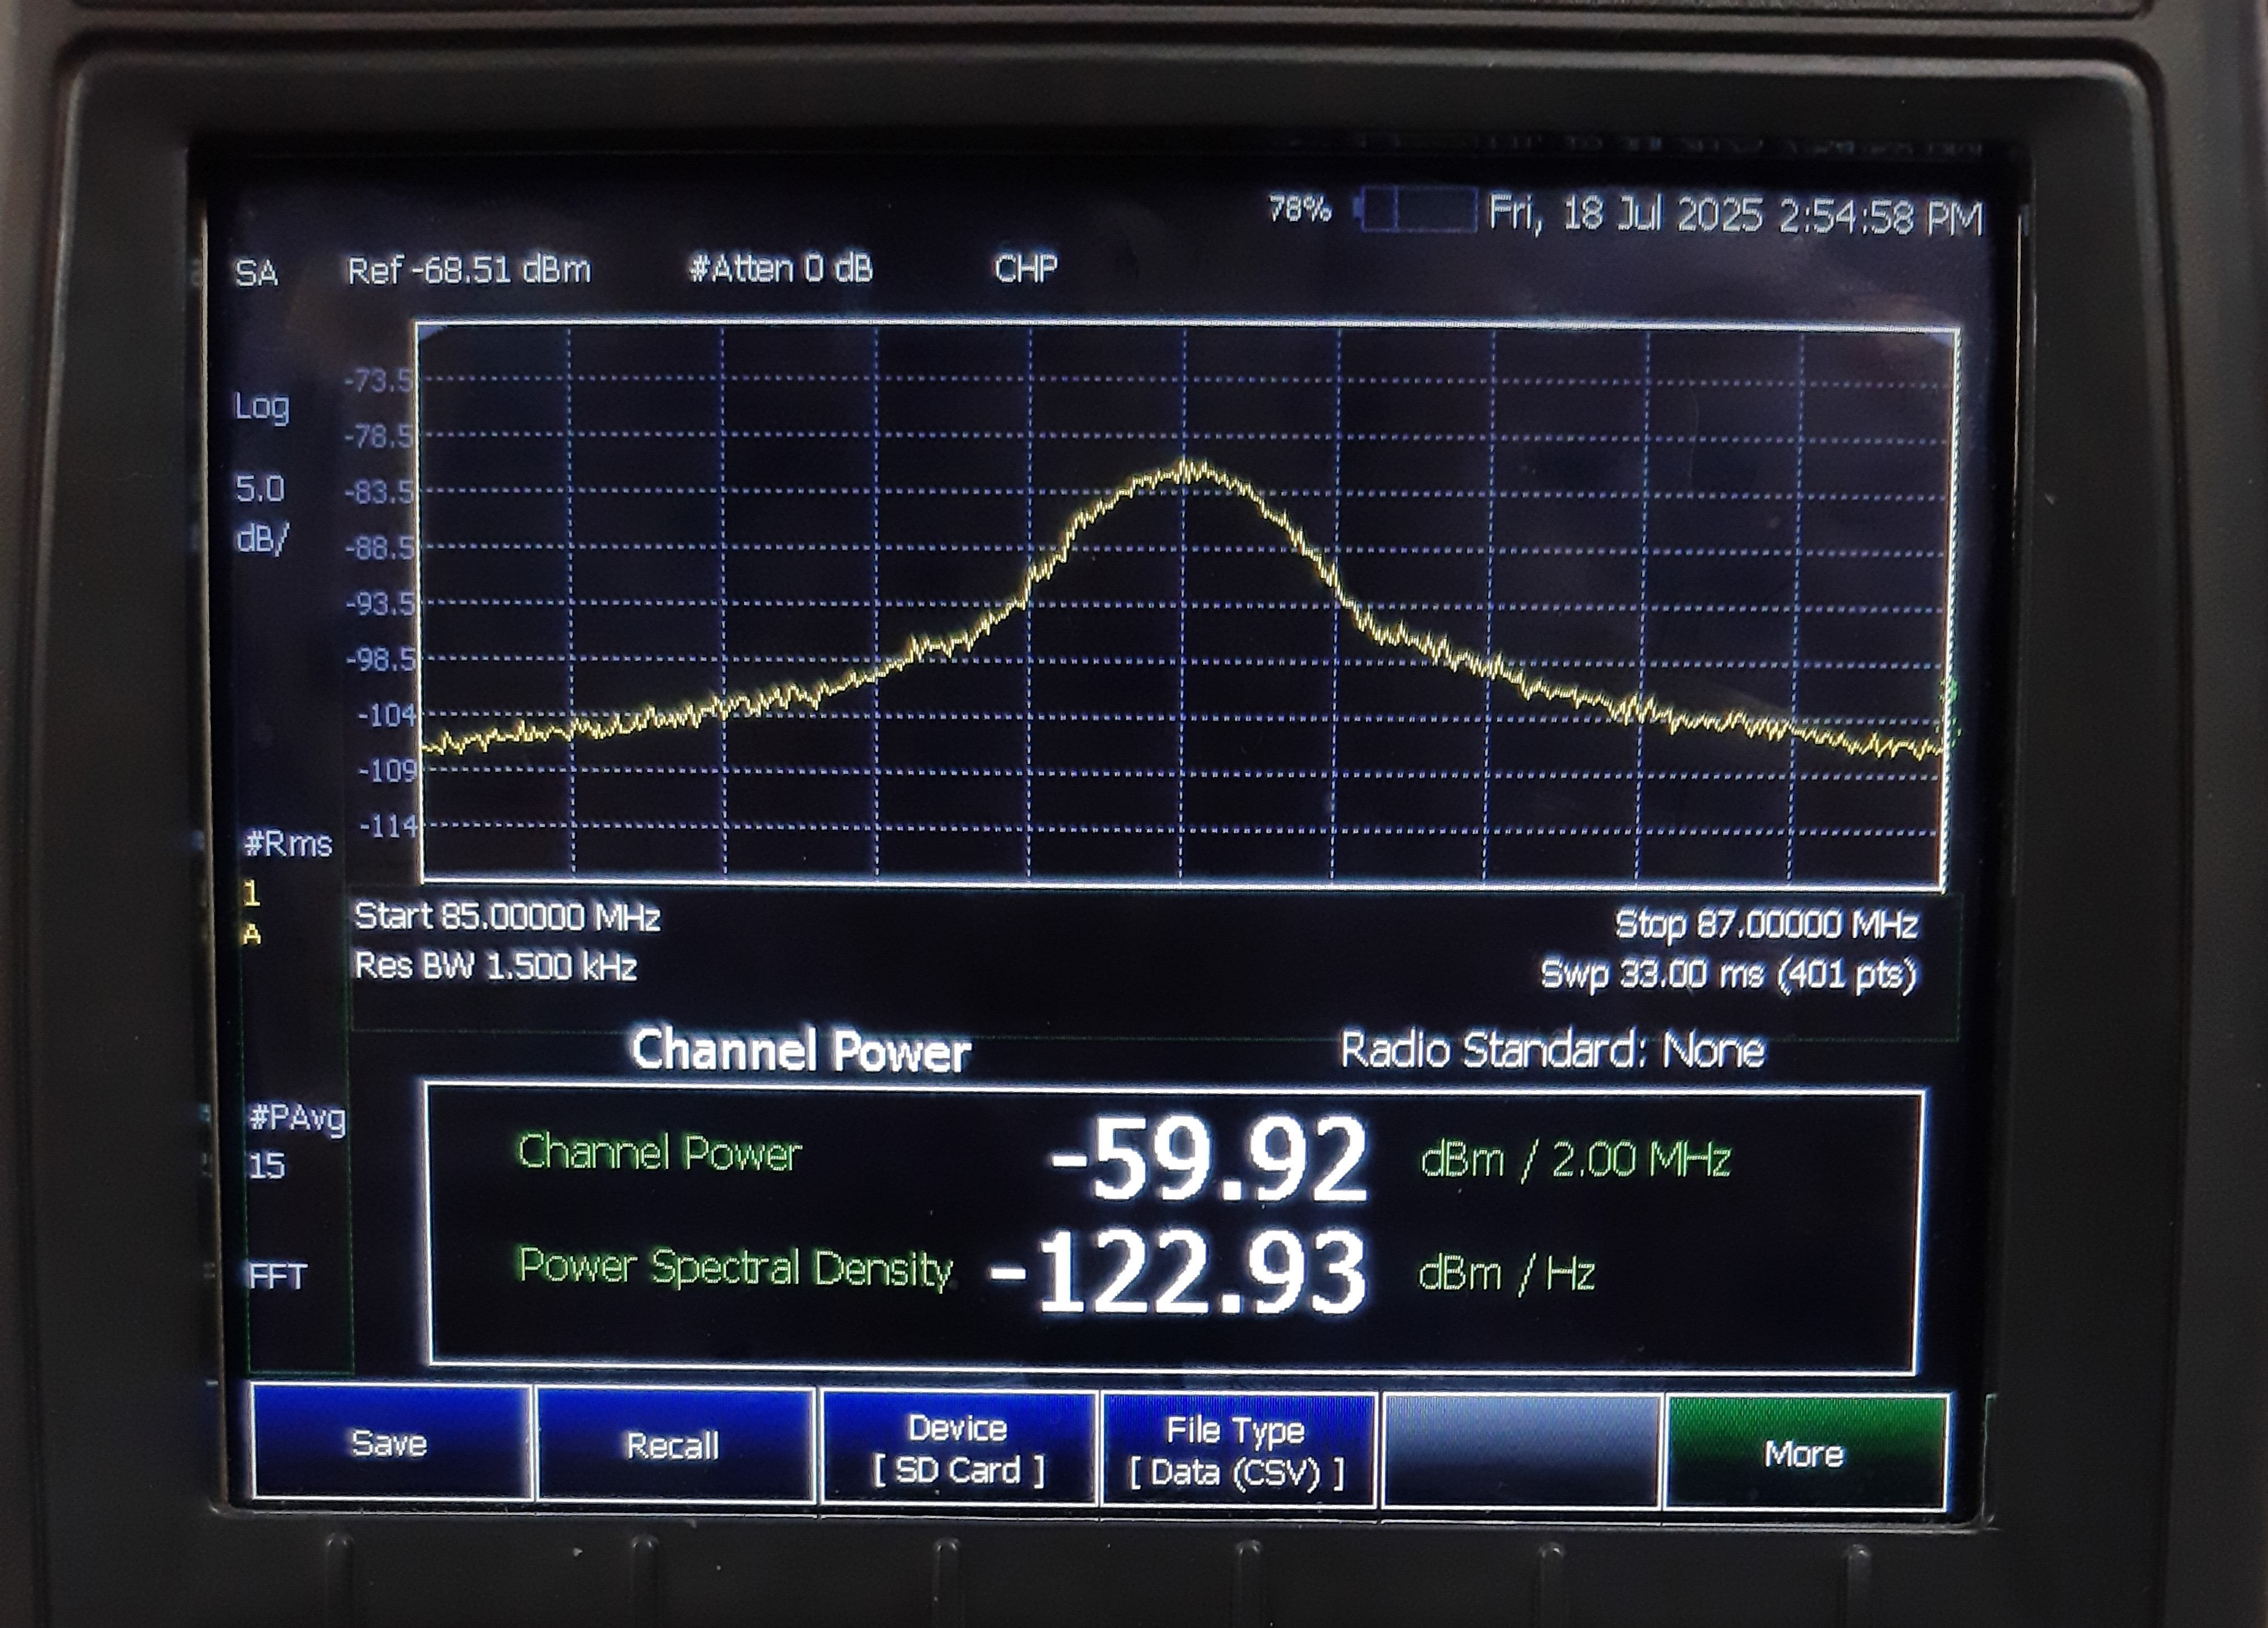
\includegraphics[width=0.4\textwidth]{media/M-S6+R0.3.jpg}
		\caption{Medición de potencia transmitiendo y con el generador de ruido a 0.3 m}
		\label{fig:M-S6+R0.3}
	\end{figure}
\end{document}